\documentclass[twoside]{report}
\usepackage[utf8]{inputenc}
\usepackage[spanish, activeacute]{babel}
\usepackage{amsmath}
\usepackage{amsfonts}
\usepackage{booktabs}
\usepackage{amssymb}
\usepackage{makecell}
\usepackage{lipsum}
\raggedbottom
\usepackage{float}
\usepackage{url}
\usepackage{rotating}
\usepackage{eurosym}
\usepackage[table,xcdraw]{xcolor}
\setcounter{secnumdepth}{3} %Profundidad en el índice de contenidos.
\usepackage{multirow}
\usepackage{multicol}
\usepackage{cite}
\usepackage{layout}
\renewcommand{\baselinestretch}{1.2}
\setlength{\parindent}{1cm}
\usepackage{helvet}
\usepackage{graphicx}
\renewcommand{\familydefault}{\sfdefault}

\addto\captionsspanish{\renewcommand{\bibname}{}}
\addto\captionsspanish{\renewcommand{\contentsname}{Índice de contenidos}}
\addto\captionsspanish{\renewcommand{\listfigurename}{Índice de figuras}}
\addto\captionsspanish{\renewcommand{\listtablename}{Índice de tablas}}

\usepackage{geometry}
\geometry{showframe=false,a4paper,left=2cm, right=1.5cm,top=1.6cm,bottom=1.5cm, includehead,includefoot}
\usepackage{fancyhdr}

\fancyhf{}
\renewcommand\headrulewidth{0pt}
\fancyhead[CO,CE]{\begin{small}Route66App: Aplicación móvil de ludificación empresarial	\end{small}\\\hrulefill}
\fancyfoot[RO, LE]{\hrulefill\\\thepage}

\fancypagestyle{plain}{%
  \fancyhf{}
  \fancyhead[CO,CE]{\begin{small}Route66App: Aplicación móvil de ludificación empresarial	\end{small}\\\hrulefill}
  \fancyfoot[RO, LE]{\hrulefill\\\thepage}
}


\pagestyle{fancy}

%%%%%%%%%%%%%%%%%%%%%%%%%%%%%%%%%%%%%%%%%%%%%USER CASE COMMANDS

\usepackage{booktabs}

\newcommand\addrow[2]{#1 &#2\\ }

\newcommand\addheading[2]{#1 &#2\\ \hline}
\newcommand\tabularhead{\begin{tabular}{lp{0.7\textwidth}}
\hline
}

\newcommand\addmulrow[2]{ \begin{minipage}[t][][t]{2.5cm}#1\end{minipage}% 
   &\begin{minipage}[t][][t]{8cm}
    \begin{enumerate} #2   \end{enumerate}
    \end{minipage}\\ }

\newenvironment{usecase}{\tabularhead}
{\hline\end{tabular}}

%%%%%%%%%%%%%%%%%%%%%%%%%%%%%%%%%%%%%%%%%%%%%%%%%%%%%%%%%%%%

%%%%%%%%%%%%%%%%%%%%%%%%%%%%%%%%%%%%%%%%%%%%%RISK MANAGEMENT

\newenvironment{risk}{\tabularhead}
{\hline\end{tabular}}

%%%%%%%%%%%%%%%%%%%%%%%%%%%%%%%%%%%%%%%%%%%%%%%%%%%%%%%%%%%%

%%%%%%%%%%%%%%%%%%%%%%%%%%%%%%%%%%%%%%%%%%%%%REQUERIMENT

\newenvironment{req}{\tabularhead}
{\hline\end{tabular}}

%%%%%%%%%%%%%%%%%%%%%%%%%%%%%%%%%%%%%%%%%%%%%%%%%%%%%%%%%%%%

%%%%%%%%%%%%%%%%%%%%%%%%%%%%%%%%%%%%%%%%%%%%%TEST

\newenvironment{test}{\tabularhead}
{\hline\end{tabular}}

%%%%%%%%%%%%%%%%%%%%%%%%%%%%%%%%%%%%%%%%%%%%%%%%%%%%%%%%%%%%



\author{Álvaro Carreras Regorigo}
\title{Route 66}
\begin{document}
\pagenumbering{gobble}
\begin{titlepage}
\begin{center}

\includegraphics[scale=0.5]{images/logoUVa}\\\vspace{1cm}
\begin{LARGE}\textbf{Universidad de Valladolid}\end{LARGE}\\
\vspace{2cm}
\begin{Huge}Escuela de Ingeniería Informática\end{Huge} \\\vspace{0.5cm}
\begin{large}\textsc{\textbf{TRABAJO FIN DE GRADO}}\end{large}\\ \vspace{2.5cm}
\begin{Large}Grado en Ingeniería Informática \\ (Mención en Ingeniería de Software)\end{Large}\\ \vspace{4cm}
\begin{Huge}\textbf{Route66App}\end{Huge}
\end{center}\vspace{2cm}
\begin{flushright}
\begin{large}Autor: \\\textbf{D. Álvaro Carreras Regorigo}\\
Tutora:\\
Dña. Margarita Gonzalo Tasis\end{large}
\end{flushright}
\end{titlepage}
\clearpage

\newpage
\thispagestyle{empty}
\mbox{}

\clearpage


\section*{Resumen}

Cada vez es más común encontrarse la ludificación aplicada a los procesos empresariales como una forma de incrementar la productividad sobre un determinado aspecto. Una de las aplicaciones más comunes es la fidelización de clientes, en donde, por medio de una serie de juegos y actividades, se incita a aumentar el consumo de los usuarios sobre la marca y esta es justa la idea fundamental sobre la que se sustenta este Trabajo de Fin de Grado.

Route66App es una aplicación nativa para dispositivos Android orientada a aplicar técnicas de ludificación empresarial de fidelización de clientes para una cadena de restaurantes de comida rápida. Se ha realizado con las últimas tecnologías propuestas por Google para el desarrollo de aplicaciones móviles: Firebase y Kotlin.


\section*{Abstract}

It is more and more common to find the gamification applied to the different business procedures as a way of increasing the productivity over a certain business aspect. One of the most common applications is the earning of customers loyalty where, thanks to different games and activities, customers are encouraged to increase the expense in the products of the brand and that is exactly the main idea of this Final Degree Project.

Route66App is a native Android application oriented to apply the business gamification techniques of earning the customers loyalty for a quick-meal restaurant chain. It has been made using the latest technologies proposed by Google for the mobile app development: Firebase and Kotlin.

\clearpage

%%%%%%%%%%%%%%%%%%%%%%%%%%%%%%%%%%%%%%%%%%%%%%%%%%
%%%%%%%%%%%%%%%%%%%%%%%Agradecimientos

\hbox{}
\vspace{7cm}
\begin{huge}
Agradecimientos
\end{huge}

\begin{flushright}
\textit{Quisiera agradecer, en primer lugar, a mi tutora del Trabajo de Fin de Grado, Dña. Margarita Gonzalo Tasis, por su dedicación e ilusión puesta en este proyecto.} \vspace{0.5cm}

\textit{En segundo lugar, a mi familia y amigos, por el apoyo que me han dado en estos cuatro años de carrera y en especial a mis padres por haberme ayudado en este trabajo a la hora de aportar ideas y opiniones.} \vspace{0.5cm}

\textit{Por último, a mis compañeros de equipo de Telefónica Investigación y Desarrollo, que me han dado la oportunidad de aprender tecnologías muy utilizadas y relacionadas con el desarrollo de aplicaciones Android.} \vspace{0.5cm}

\textit{Gracias a todos.}
\end{flushright}

\newpage
\thispagestyle{empty}
\mbox{}

\clearpage

\tableofcontents

\listoffigures
 
\listoftables

\clearpage

\pagenumbering{arabic}


\chapter{Introducción y contexto.}
\section{Introducción y objetivos.}

\subsection{Introducción.}

La ludificación consiste, según IEBSchool \cite{iebschoolGami} en \textit{“el uso de mecánicas de juego en un contexto de no juego para conducir el comportamiento de los participantes (mediante la participación, la interacción, la adicción o, incluso, la competición) hacia la consecución de un determinado objetivo de negocio”}. 

Aunque habitualmente se ha enfocado la ludificación al área comercial o de ventas de cara a los clientes, (como por ejemplo el \cite{monopolymcdo} \textit{Monopoly Ganador de McDonalds}), existen también ejemplos en la educación, en las relaciones con los proveedores e, incluso, para incrementar el número de ventas en un centro comercial, (ludificación orientada a los empleados), tal como se recoge en el Trabajo de Fin de Grado de la alumna del Grado en Ingeniería Industrial, \cite{anatfg} Dña. Ana Ruiz Caballero.

Hoy en día, miles de compañías utilizan la ludificación en sus procesos empresariales desde sus relaciones con los empleados hasta con los clientes, pasando por sus comerciales. La ludificación realmente funciona y, por increíble que parezca, es muy efectiva. De hecho, no son pocos los ejemplos de una aplicación más que satisfactoria de la misma. Así, en 2011, \cite{accentureGami} Volkswagen decidió inventar en China, su mercado más importante, una nueva versión de su \textit{“people’s car“} y para ello contó con la ayuda de sus clientes, a quienes ofreció una herramienta de diseño y un sistema de puntuaciones. El resultado de este proyecto fue la obtención de más de 50.000 propuestas diferentes. Otro caso que merece la pena reseñar es el de Correos \cite{confidencialcorreosgami}, que en 2012 rediseñó su web y se planteó o bien contratar a una empresa por miles de euros, bien, plantear un sistema de ludificación en el que los empleados propusieran nuevos diseños a cambio de pequeños regalos. Esta segunda opción fue la elegida (se presentaron más de 50.000 ideas en un tiempo récord), y esto supuso un ahorro de un 70\% frente a la primera alternativa. 

El caso más destacable en nuestro país es el de \cite{bbvag} BBVA Game, una plataforma de ludificación asociada a la banca virtual. En ella, los usuarios consiguen puntos al superar distintos retos como consultar movimientos, domiciliar la nómina, realizar transferencias, etcétera. Igualmente, también se pueden conseguir incentivos por compartir un mensaje en redes sociales,  invitar a amigos o contratar productos, que es posible canjear por premios directos o por participaciones en los sorteos que realizan. El resultado de este proyecto fue un éxito rotundo, ya que consiguieron 100.000 nuevos clientes en los nueve primeros meses y aumentaron el uso de la plataforma por parte de sus clientes ya existentes.

\subsection{Objetivos.}

El propósito de este Trabajo Fin de Grado es el de realizar una aplicación Android basada en un sistema de ludificación para un restaurante de comida rápida, partiendo de la idea desarrollada en el \cite{cristinatfg} Trabajo de Fin de Grado de Dña. Cristina Martínez Martínez. Los objetivos concretos de la aplicación vendrán detallados en el documento de análisis.

Este Trabajo Fin de Grado detallará el desarrollo, análisis, diseño e implementación de la parte cliente del sistema informático en cuestión y se ha diseñado para que esta cambie las diferentes misiones y desafíos de acuerdo con los parámetros que el administrador del sistema establezca en el \textit{backend} (parte de gestión).

\subsection{Motivación.}

La motivación es doble, por un lado, analizar, diseñar e implementar un sistema de ludificación, diseñado por una antigua alumna de esta Universidad para completar así una de las líneas futuras propuestas por la misma en su Trabajo de Fin de Grado, y por otro, se busca desarrollar un sistema de ludificación que permita a los alumnos del Grado en Organización Industrial de nuestra Universidad poner en marcha y probar un sistema de este tipo, que no tiene alternativas de licencia de prueba para estudiantes en el mercado.

\section{Análisis de aplicaciones similares}

Se han analizado diversas aplicaciones de restaurantes de comida rápida presentes en España, con el fin de conocer cómo son y si han implementado técnicas de ludificación a las mismas. Como se verá más adelante, los sistemas de ludificación aplicados en estos ejemplos son bastante básicos y no permiten extraer todo el potencial que podrían tener.

\subsection{Análisis aplicaciones de restaurantes de comida rápida.}
\subsubsection{McDonald's}

\begin{figure}[H]
\begin{center}
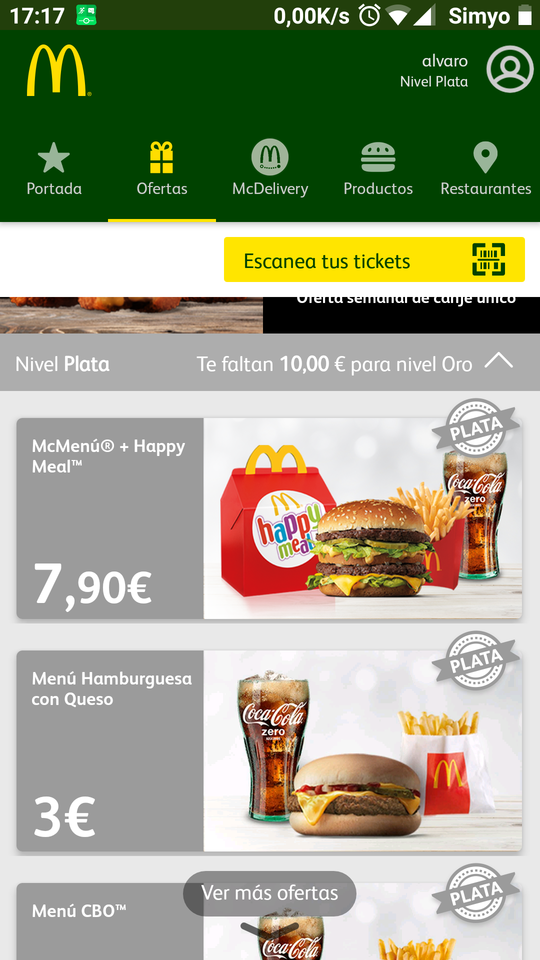
\includegraphics[scale=0.25]{images/restaurantes/mcdo0.png}
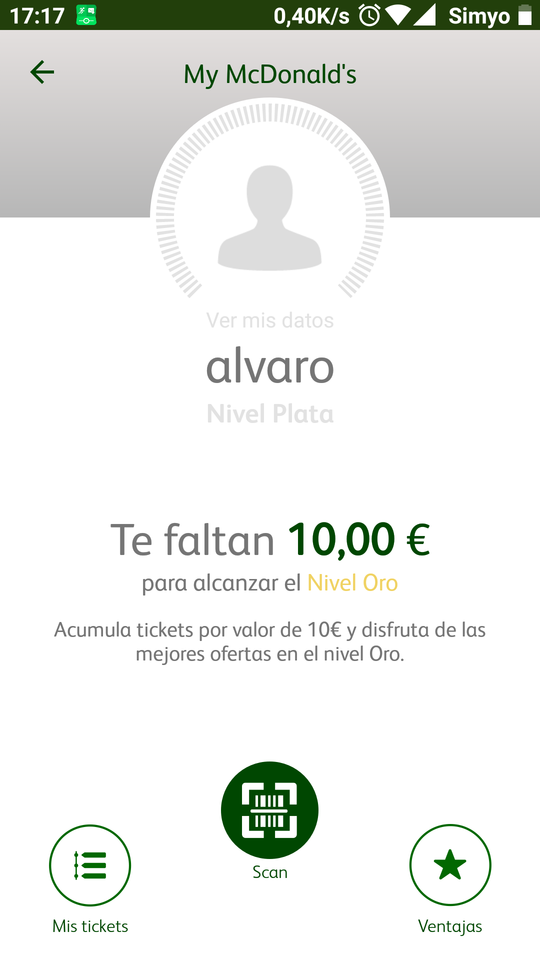
\includegraphics[scale=0.25]{images/restaurantes/mcdo1.png}
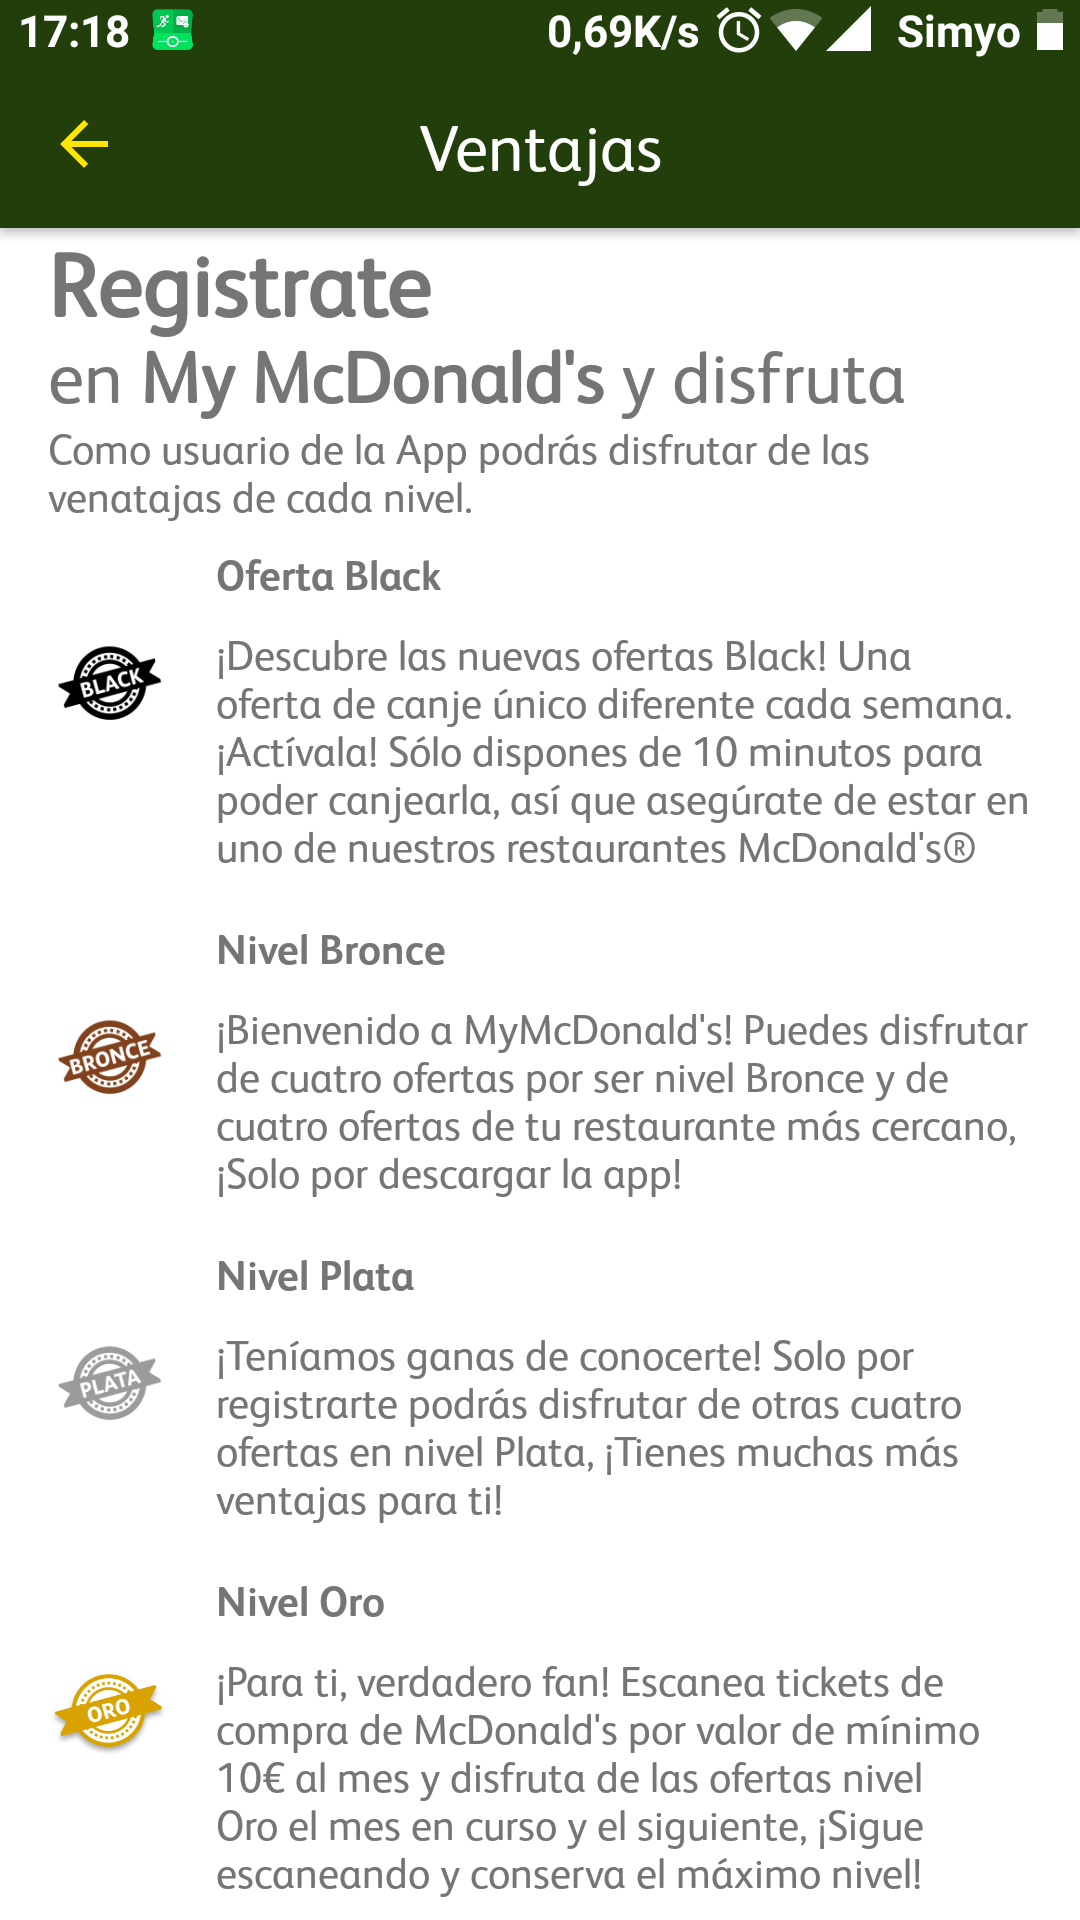
\includegraphics[scale=0.25]{images/restaurantes/mcdo3.png}
\caption{Capturas de pantalla de la aplicación \textit{“McDonald's España - Ofertas“}.} \cite{mcdo}
\end{center}
\end{figure}

\begin{itemize}
\item \textbf{Aplicación estudiada:} \cite{mcdo} \textit{McDonald's España - Ofertas.}
\item \textbf{Análisis:} 
La aplicación móvil McDonalds ofrece un gran número de funcionalidades entre las que se encuentran un servicio de ofertas, canjeo de cupones, listado de la carta de productos o envío de pedidos a domicilio. 

El sistema de ludificación implementado es bastante básico ya que su estrategia se basa en utilizar un sistema por niveles (oro, plata y bronce), en el que cuanto mayor sea el nivel del usuario, mejores ofertas se pueden encontrar. Para poder subir de nivel, será necesario escanear los tickets de compra y llegar a un mínimo de gasto. Durante el tiempo que la he tenido instalada, me ha pedido dar la opinión de la app por correo electrónico a cambio de obtener un obsequio.

\item \textbf{Puntos fuertes:}
	\begin{itemize}
	\item Promueve el consumo de los clientes en los restaurantes de la cadena, recomendándoles hacer un determinado gasto para poder mantenerse en el mismo nivel.
	\item Ofertas \textit{“Black“}: Son ofertas que se activan solo durante diez minutos y hay que estar presente en el local en ese momento para canjearlas.
	\end{itemize}
\item \textbf{Puntos débiles:}
	\begin{itemize}
	\item Se limita al consumo y no a promocionar la marca por redes sociales ayudándose de los clientes.
	\item Las promociones solo se pueden hacer efectivas en los establecimientos físicos, no en pedidos por Internet.
	\item No existe ningún historial de pedidos.
	\end{itemize}
\end{itemize}


\subsubsection{Burger King}

\begin{figure}[H]
\begin{center}
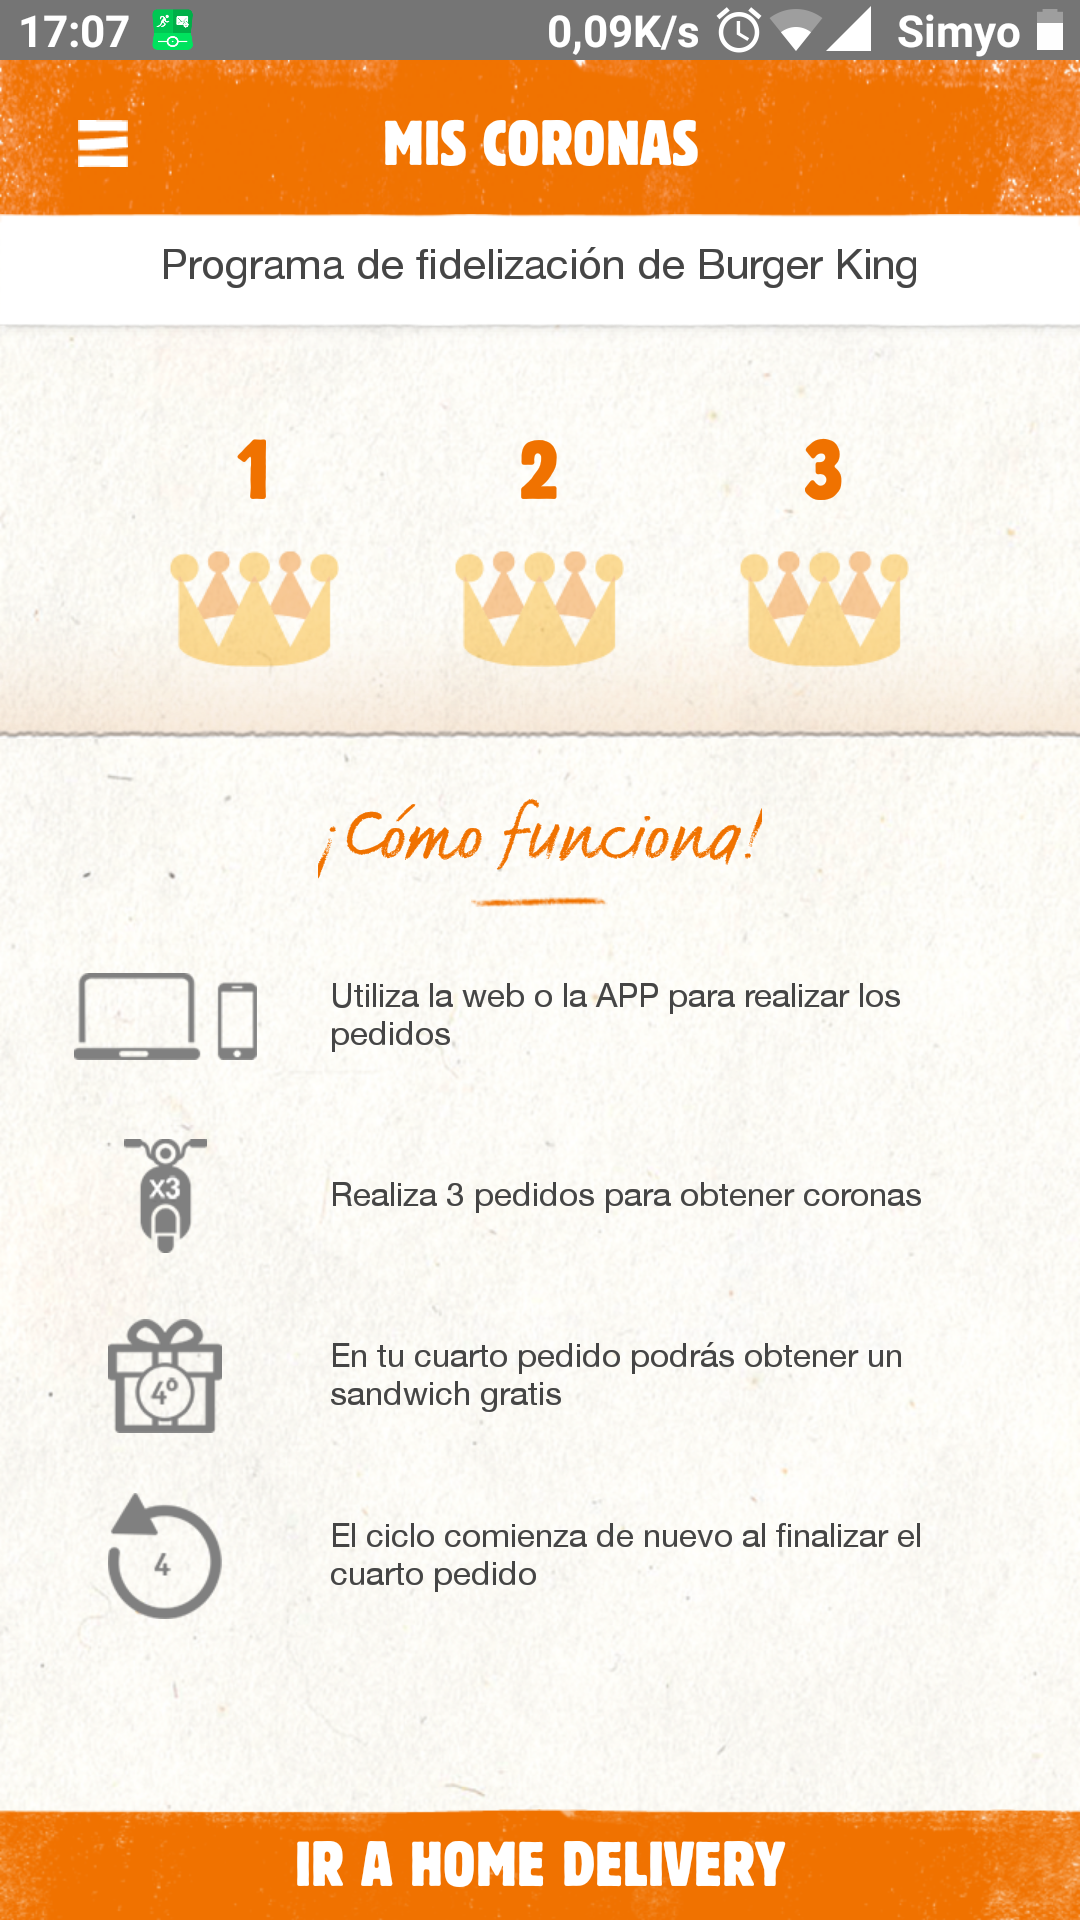
\includegraphics[scale=0.25]{images/restaurantes/burry0.png}
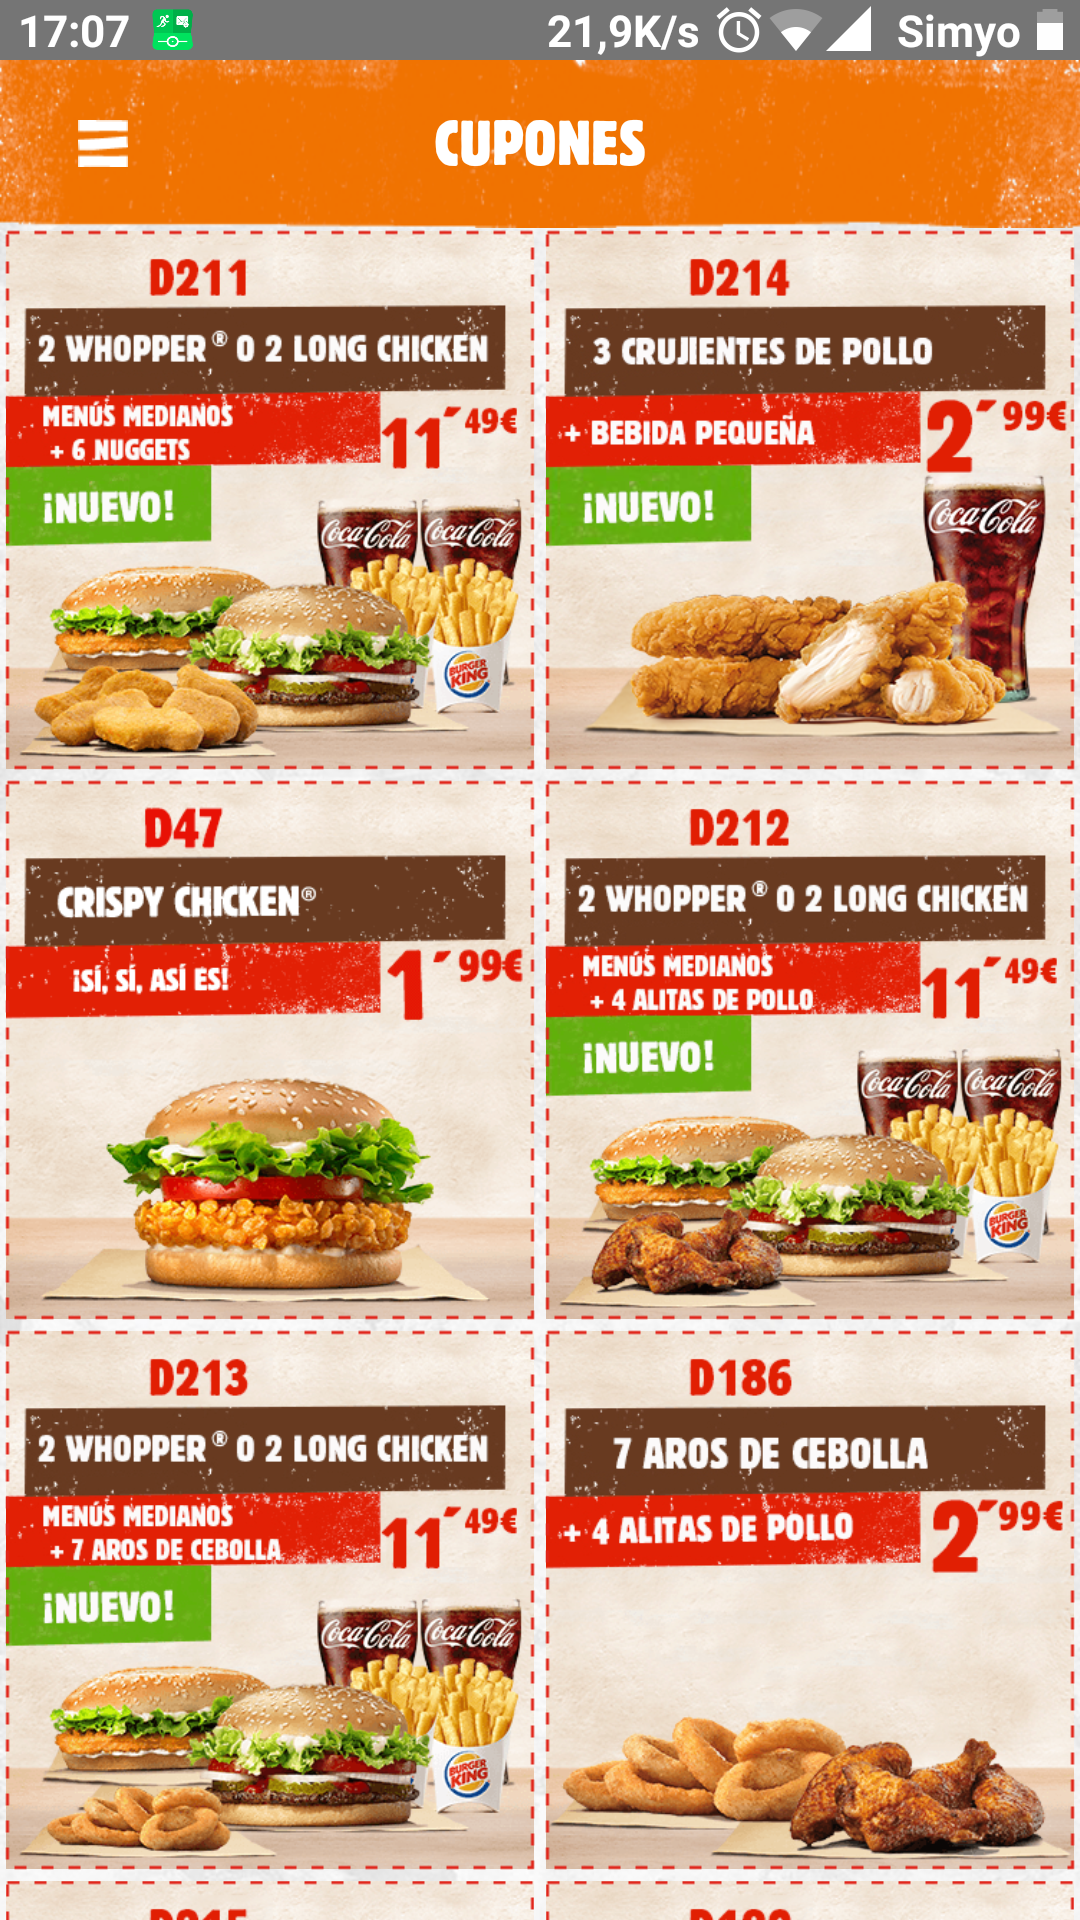
\includegraphics[scale=0.25]{images/restaurantes/burry1.png}
\caption{Capturas de pantalla de la aplicación \textit{“BURGER KING® España“}.} \cite{burgerk}
\end{center}
\end{figure}

\begin{itemize}
\item \textbf{Aplicación estudiada:} \cite{burgerk} \textit{BURGER KING® España.}
\item \textbf{Análisis:} 
Al igual que McDonalds, ofrece un sistema de fidelización llamado \textit{“Mis Coronas“}, consistente en que cada tres pedidos realizados por medio de la app móvil o el sitio web de Burger King, se acumulan coronas y cada cuatro se consigue una hamburguesa gratis. Además, invitan a registrarse en la app y con el historial de pedidos efectúan ofertas personalizadas al cliente.

Las opciones de esta app están bastante limitadas: conseguir un listado de restaurantes, realizar pedidos a domicilio, ver la carta de productos o visualizar un listado de cupones o promociones.

\item \textbf{Puntos fuertes:}
	\begin{itemize}
	\item Avisa mediante notificaciones \textit{PUSH} de nuevas ofertas.
	\item Solicita seguir a la marca por redes sociales (\textit{Facebook}).
	\item Tiene un sistema de fidelización para sus pedidos \textit{online}.
	\item Permite visualizar el historial de pedidos por Internet.
	\end{itemize}
\item \textbf{Puntos débiles:}
	\begin{itemize}
		\item La parte de fidelización está solo dedicada a la realización de pedidos por Internet.
		\item Las promociones son muy similares, independientemente del perfil del cliente.
		\item No está orientada a que el cliente realice un determinado consumo.
		\item No se pueden aplicar los cupones de la aplicación a pedidos a domicilio.
	\end{itemize}
\end{itemize}

\subsubsection{KFC}

\begin{figure}[H]
\begin{center}

\includegraphics[scale=0.25]{images/restaurantes/kfc0.png}
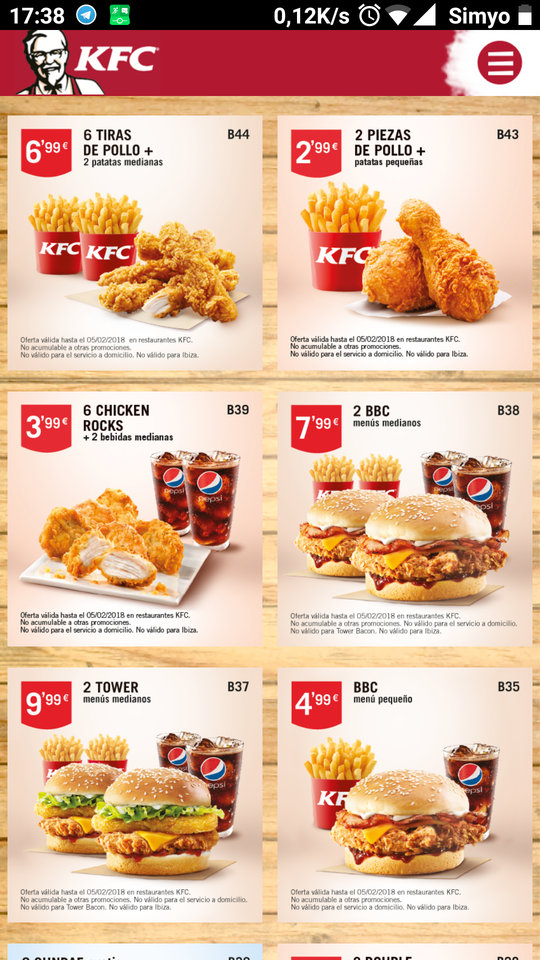
\includegraphics[scale=0.25]{images/restaurantes/kfc1.png}
\caption{Capturas de pantalla de la aplicación \textit{“KFC España–ofertas cerca de ti“}.} \cite{kfcapp}
\end{center}
\end{figure}


\begin{itemize}
\item \textbf{Aplicación estudiada:} \cite{kfcapp} \textit{KFC España–ofertas cerca de ti.}
\item \textbf{Análisis:} 

Es una de las aplicaciones más simples de las estudiadas pues se limita a poner una carta de productos, un listado de restuarantes y una opción para obtener ofertas.

\item \textbf{Puntos fuertes:}
	\begin{itemize}
	\item Notificaciones \textit{PUSH} para alertar al cliente de nuevas ofertas y promociones.
	\end{itemize}
\item \textbf{Puntos débiles:}
	\begin{itemize}
	\item No tiene un sistema de fidelización.
	\end{itemize}
\end{itemize}

\subsubsection{VIPS}

\begin{figure}[H]
\begin{center}

\includegraphics[scale=0.25]{images/restaurantes/vips0.png}

\includegraphics[scale=0.25]{images/restaurantes/vips1.png}
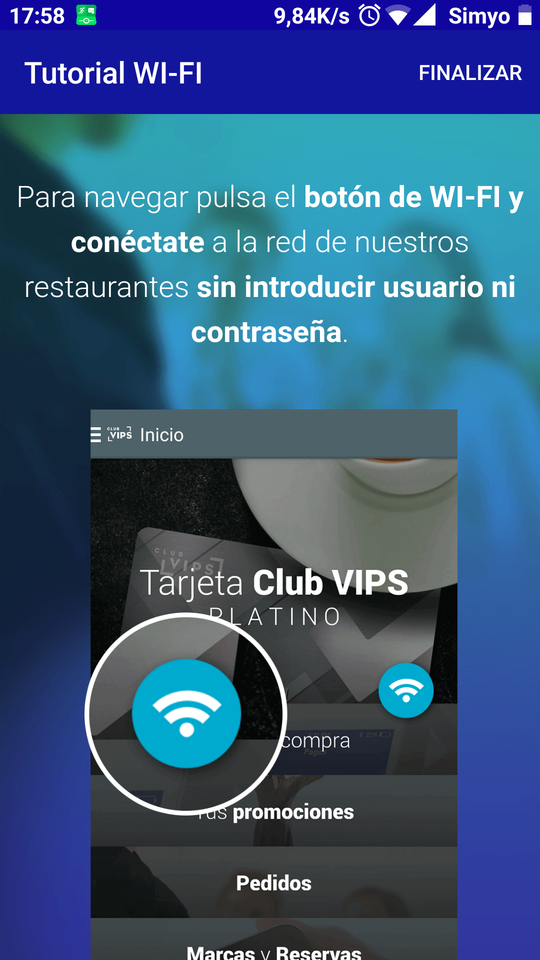
\includegraphics[scale=0.25]{images/restaurantes/vips2.png}
\caption{Capturas de pantalla de la aplicación \textit{“Club VIPS: Promociones y pedidos Take Away“}.} \cite{vipsapp}
\end{center}
\end{figure}

\begin{itemize}
\item \textbf{Aplicación estudiada:} \cite{vipsapp} \textit{Club VIPS: Promociones y pedidos Take Away.}
\item \textbf{Análisis:} 
La aplicación de la cadena VIPS es, sin lugar a dudas, la más completa de las analizadas.

Para fidelizar clientes utiliza el servicio ClubEuroVIPS, en el que ofrece un \textit{cashback} de un 3\%, pudiendo duplicarse bajo ciertas condiciones como aumentar el consumo o hacerlo en determinadas franjas horarias. Además ofrece un sistema de clasificación de usuarios por niveles de gasto (niveles clásico, oro y platino) a partir de los cuales podremos obtener \textit{WiFi} Premium, bebidas extras o puntos extras.

Paralelamente, la aplicación invita al usuario a sus lanzamientos o estrenos de nuevos productos. Por ejemplo “\textit{te invitamos a nuestras hamburguesas del Chef o a nuestras nuevas pizzas Chicago Style}” o “\textit{te invitamos a probar nuestras pizzas}” y se pueden encontrar funcionalidades propias de un restaurante que apuesta por el crecimiento de su app móvil, como son la posibilidad de pagar desde la app, la funcionalidad \textit{Shake-It}, que consiste en realizar su pedido favorito con solo agitar su teléfono móvil, o la opción de guardar promociones en la aplicación. Además de permitir realizar pedidos online del tipo \textit{take-away}.
\item \textbf{Puntos fuertes:}
	\begin{itemize}
	\item La aplicación integra la tarjeta \textit{Club VIPS}, que permite sumar puntos gracias a las compras hechas en restaurantes de la marca.
	\item Se puede duplicar el valor de los puntos del  \textit{Club VIPS} bajo condiciones específicas.
	\item Notificaciones \textit{PUSH} para informar al cliente de nuevas ofertas y promociones.
	\item Historial de pedidos.
	\item Integra un sistema para conectarse automáticamente con las redes \textit{WiFi} de los restaurantes de la marca. Posibilidad de tener \textit{WiFi} Premium en caso de alcanzar un cierto consumo.
	\item Permite capturar nuevas promociones escaneando el código \textit{QR} de la publicidad.
	\item Invitaciones a eventos por el hecho de ser usuario de un determinado nivel.
	\item Clasificación del usuario por niveles basándose en el consumo que se hace en los restaurantes.
	\item Se realiza \textit{cashback} en los pedidos realizados siendo socio del \textit{Club VIPS}.
	\item Se puede conseguir hasta un 25\% de descuento al invitar a usuarios a hacerse socios del \textit{Club VIPS}.
	\end{itemize}
\item \textbf{Puntos débiles:}
	\begin{itemize}
	\item No existe ningún juego ni interacción con redes sociales.
	\end{itemize}
\end{itemize}

\subsubsection{Pans \& Company}

\begin{figure}[H]
\begin{center}

\includegraphics[scale=0.25]{images/restaurantes/pans0.png}
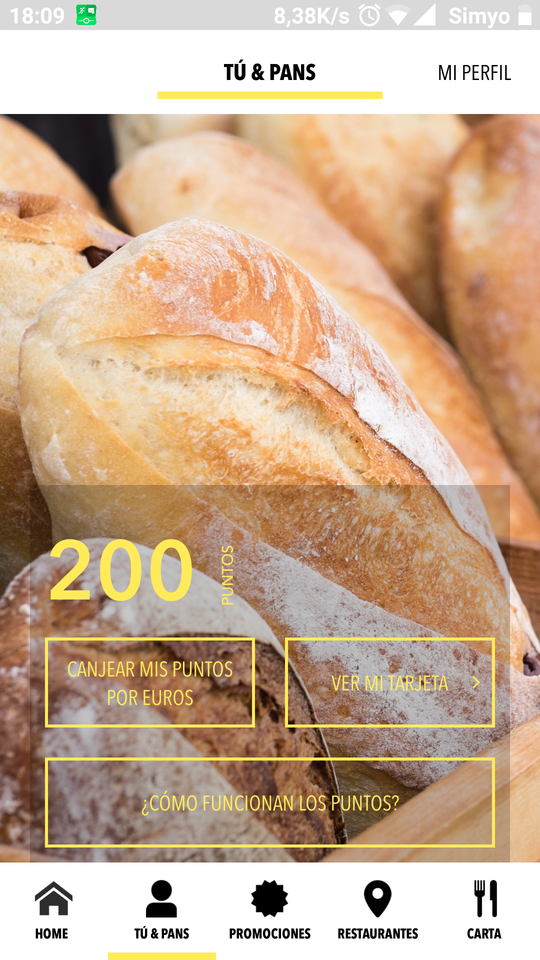
\includegraphics[scale=0.25]{images/restaurantes/pans1.png}
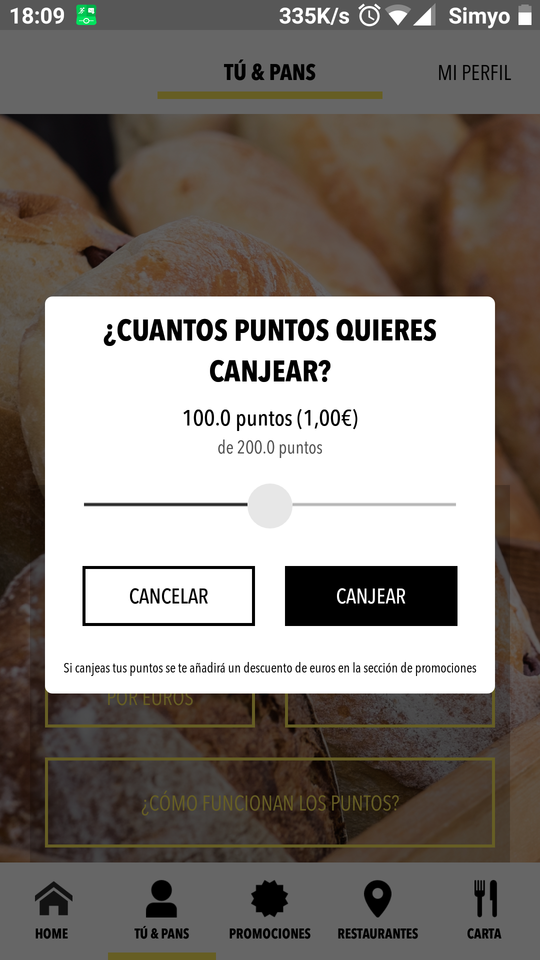
\includegraphics[scale=0.25]{images/restaurantes/pans2.png}
\caption{Capturas de pantalla de la aplicación \textit{“Pans \& Company“}.} \cite{pansapp}
\end{center}
\end{figure}

\begin{itemize}
\item \textbf{Aplicación estudiada:} \cite{pansapp} \textit{Pans \& Company.}
\item \textbf{Análisis:} 
Pans \& Company ofrece únicamente una tarjeta de fidelidad integrada en la misma app. Esta tarjeta básicamente consiste en un código QR que el usuario puede mostrar en caja para acumular puntos que, posteriormente, se podrán convertir en dinero. Además, se realizarán ofertas personalizadas.

Sus funcionalidades son las típicas de una aplicación de esta categoría: listado de restaurantes, ofertas y listado de la carta.
\item \textbf{Puntos fuertes:}
	\begin{itemize}
	\item Notificaciones \textit{PUSH} para alertar al cliente de nuevas ofertas y promociones.
	\item La aplicación integra una tarjeta de fidelización en el que se acumulan puntos a la hora de realizar compras. Los puntos se podrán canjear posteriormente por descuentos en compras en los restaurantes.
	\end{itemize}
\item \textbf{Puntos débiles:}
	\begin{itemize}
	\item No cuenta con interacción entre usuarios ni redes sociales, se limita a la tarjeta de fidelización.
	\end{itemize}
\end{itemize}

\subsubsection{Foster's Hollywood}

\begin{figure}[H]
\begin{center}

\includegraphics[scale=0.25]{images/restaurantes/foster0.png}

\includegraphics[scale=0.25]{images/restaurantes/foster1.png}
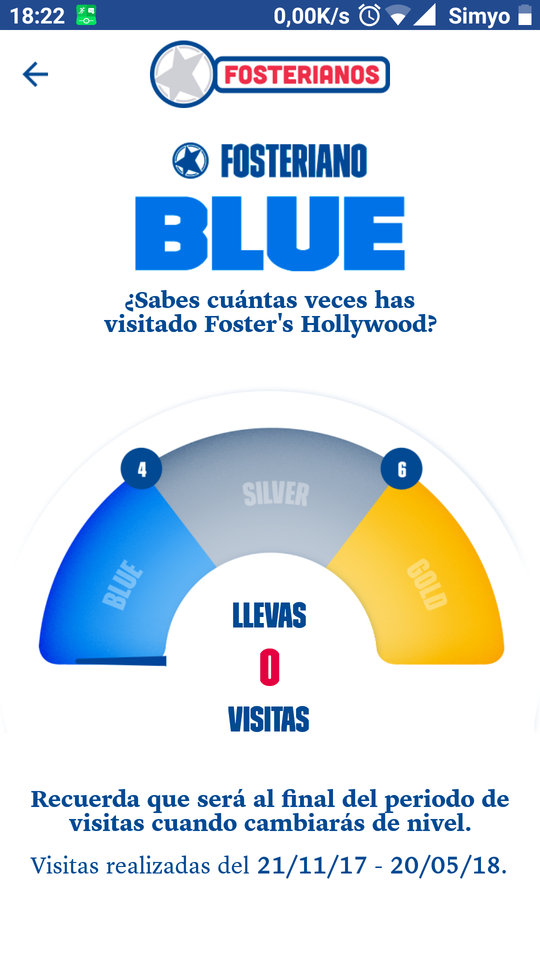
\includegraphics[scale=0.25]{images/restaurantes/foster2.png}
\caption{Capturas de pantalla de la aplicación \textit{“Foster's Hollywood“}.} \cite{fostersh}
\end{center}
\end{figure}

\begin{itemize}
\item \textbf{Aplicación estudiada:} \cite{fostersh} \textit{Foster's Hollywood.}
\item \textbf{Análisis:} 
El sistema de fidelización de clientes de Foster's Hollywood se basa en un sistema de niveles (\textit{blue}, \textit{silver} y \textit{gold}), en el que cuanto mejor sea el nivel, mayores ventajas tendrá el usuario: postre de regalo, descuentos de ocio (en empresas asociadas), o incluso, promoción por el cumpleaños. Para poder aumentar de nivel será necesario ir un número de veces a los establecimientos de la cadena. 

Se nos identificará como clientes mediante la tarjeta Foster's Hollywood, un código QR localizado en la aplicación y que el cliente simplemente debe enseñar al realizar el pago, con el fin de que la compra quede asociada a su usuario. Por otra parte, también es posible visualizar la carta del restaurante o ver el listado de restaurantes, así como realizar el pedido online.
\item \textbf{Puntos fuertes:}
	\begin{itemize}
	\item Notificaciones \textit{PUSH} para informar al cliente de nuevas ofertas y promociones.
	\item Sistema de fidelización basado en niveles e integrado en la aplicación.
	\end{itemize}
\item \textbf{Puntos débiles:}
	\begin{itemize}
	\item No cuenta con interacción entre usuarios ni redes sociales, se limita al sistema de fidelización.
	\end{itemize}
\end{itemize}

\subsection{Conclusiones extraídas}

Del análisis de las anteriores aplicaciones, pueden extraerse las siguientes conclusiones:
\begin{itemize}

\item Ninguna emplea un sistema de ludificación avanzado tal y como se propone en este trabajo.

\item Los sistemas de fidelización de clientes son bastante limitados siendo, en muchos casos, una simple tarjeta virtual donde acumular puntos.

\item Todas ofrecen un sistema para obtener ofertas.

\item Las aplicaciones se limitan a la interacción Usuario-Empresa, ninguna emplea las redes sociales para aumentar su base de usuarios.

\item La mayoría de las aplicaciones (todas exceptuando Burger King y KFC) promueven que el usuario vuelva al local, mediante la realización de ofertas específicas para ello. Irían dirigidas a un perfil de jugador de tipo \textit{triunfador}, de acuerdo con la \cite{iebsctj} teoría de Bartle.
\end{itemize}

\section{Estructura de la memoria}

Este trabajo está divido en cuatro partes y, a su vez, en secciones y subsecciones, abarcando así los distintos documentos recogidos en esta memoria:

\begin{enumerate}
\item Capítulo I. Introducción y Objetivos: incluye una breve descripción de lo que es la ludificación, así como un resumen de la propuesta realizada por la diseñadora del sistema de ludificación sobre la que está basado el proyecto. Finalmente, también contiene un análisis de aplicaciones de restaurantes de comida rápida que operan en España, con la finalidad de estudiar si estos incluyen o no un sistema de ludificación.

\item Capítulo II. Herramientas utilizadas: justificación del empleo de alguna de ellas. 

\item Capítulo III. Route66App: es la parte más importante del proyecto porque incluye la gran mayoría de los documentos, como el Plan de Desarrollo de Software, el documento de análisis, el documento de diseño y todos aquellos detalles de la implementación que merecen la pena reseñar.

\item Capítulo IV. Conclusiones y líneas futuras.

\item Webgrafía y bibliografía.

\item Anexos

\end{enumerate}

\section{Propuesta.}
Este Trabajo de Fin de Grado (T.F.G) estará centrado en el T.F.G. \cite{cristinatfg} “\textit{Estudio de ludificación en una empresa para mejorar la fidelización de los clientes}”, elaborado por Dª Cristina Martínez Martínez, graduada durante el curso 2016-2017 en Ingeniería de Organización Industrial por la Universidad de Valladolid.  

El trabajo de esta alumna, centrado en el diseño de un sistema de ludificación aplicado a un posible caso real,(restaurante de comida americana), tenía el problema de la imposibilidad de llevarlo a cabo con herramientas profesionales, dado su coste y a la falta de disponibilidad de las mismas. Por este motivo, el T.F.G. se tuvo que defender contando solo con una serie de prototipos basados en un sistema web. 

Como la ludificación es un área en investigacion que en experiencias anteriores ha obtenido muy buenos resultados, la tutora del T.F.G., Dña. Margarita Gonzalo Tasis, propuso la realización de este proyecto. Por otro lado, el resultado del mismo puede servir a alumnos de otras facultades de nuestra Universidad para poder utilizar una herramienta de ludificación real.

\subsection{Resumen de “Estudio de ludificación en una empresa para mejorar la fidelización de los clientes”}

Se propone la realización de un sistema de ludificación para una cadena de restaurantes de comida americana, que cuenta con un conjunto de franquicias repartidas por todo el territorio español. Es una empresa con muy buenos resultados económicos y que está respaldada por una amplia y sólida base de clientes para quienes decide elaborar una aplicación que mejore la opinión de los mismos sobre la marca, ya que han llegado críticas sobre el sistema vigente de cupones y descuentos.

Finalmente, el equipo directivo decide encargar una aplicación basada en la ludificación cuyos objetivos son los siguientes:

\begin{enumerate}
\item Aumentar la fidelización de los clientes.
\item Incentivar las ventas.
\item Mejorar la imagen de la marca en redes sociales.
\item Conseguir nuevos clientes.
\item Mejorar la confianza y satisfacción del cliente. 
\end{enumerate}

Se medirá el cumplimiento de los objetivos anteriores mediante el cálculo de una serie de ratios.\\

\textbf{Público objetivo}\\

El público objetivo estará formado por hombres y mujeres con edades comprendidas entre los doce y los cincuenta y cinco años. 
Los conocimientos tecnológicos esperados en este grupo de edad no tienen por qué ser altos, considerándose suficientes, conocimientos básicos en uso de \textit{smartphones} y de aplicaciones móviles. En el caso en el que nos encontramos, la aplicación que se va a desarrollar estará enfocada a ser ejecutada sobre terminales de tipo Android.

Los potenciales usuarios de la aplicación la utilizarán para conseguir recompensas y descuentos derivados del uso de la misma.

Por último, con el fin de fidelizar a un mayor número de clientes, y de acuerdo con la \cite{iebsctj} teoría de Bartle, se realizarán actividades que permitan satisfacer las necesidades de los cuatro tipos de jugador.\\

\textbf{Roles}\\

Se proponen dos tipos de roles: Administrador y Cliente.

Este trabajo se centrará en el rol cliente. El administrador tendrá su protagonismo en la parte de gestión, que no está incluida en este proyecto.\\

\textbf{Descripción del juego}\\

El juego se escenifica en la Ruta 66 americana que alude así la temática del restaurante. Se dividirá el camino en once etapas o niveles correspondientes a las principales ciudades por las que pasa esta vía y, para avanzar, el cliente deberá completar una serie de actividades, que además, otorgarán insignias, logros y premios. Cabe destacar que la dificultad de los niveles irá aumentando gradualmente, con el objetivo de no perder la motivación.

\begin{table}[H]
\begin{multicols}{4}
\begin{enumerate}
\item Chicago.
\item Springfield.
\item St. Louis.
\item Tulsa.
\item Oklahoma City.
\item Amarillo.
\item Santa Fe.
\item Albuquerque.
\item Flagstaff.
\item Williams.
\item Los Ángeles.
\end{enumerate}
\end{multicols}
\caption{Ciudades o niveles de la aplicación.}
\end{table}


Todos los niveles excepto el de Chicago tendrán un planteamiento similar:
\begin{itemize}
\item Nivel 1. Chicago: Compuesto por las siguientes actividades:
	\begin{itemize}
		\item Configuración del perfil del jugador.
		\item Crear un equipo.
		\item Seguir en redes sociales la página del restaurante.
		\item Puntuar la aplicación en la tienda de aplicaciones.
		\item Comentar la aplicación en la tienda de aplicaciones.
	\end{itemize}
\item Resto de niveles: Consistirán en diez misiones:
	\begin{itemize}
		\item Misiones de nivel social: consistirán en tareas como compartir el progreso, subir una foto hecha en el restaurante a las redes sociales, enviar invitaciones, etcétera.
		
		\item Misiones de minijuegos: serán dos casillas y consistirá en jugar a un minijuego de un perfil de jugador.
		
		\item Misiones de consumo: el jugador deberá realizar consumiciones en los restaurantes de la cadena. Avanzará más o menos casillas en función del gasto que realice.
		
		\item Misiones de retos especiales: en días señalados, los jugadores podrán participar en retos creados específicamente para ese día.
	\end{itemize}
\end{itemize}
\vspace{1cm}
\textbf{Recompensas}\\

Hay tres tipos de recompensa:
\begin{itemize}

\item Puntos: el usuario obtendrá diez puntos por cada casilla que avance. Y la suma total se agrupará en tres categorías: consumo, social y competitivo.

\item Insignias: cuando el jugador haya completado un nivel obtendrá una insignia (matrícula de la ciudad asociada). Habrá otras insignias, como la familiar o las de grupo, que podrá imponer el administrador del sistema.

\item Premios: los premios serán regalos. Se desbloquearán cuando el usuario haya completado un nivel o haya realizado algún reto especial.

\end{itemize}

\textbf{Perfiles de jugador\cite{iebsctj}}\\ 

Se ha aplicado la teoría de Bartle para clasificar los jugadores en cuatro categorías:
\begin{itemize}

\item Triunfador: tendrá como objetivo llevar a cabo las misiones y obtener los premios o recompensas.
\item Explorador: son jugadores que les gusta descubrir o aprender cosas nuevas.
\item Socializadores: más que interés en conseguir los logros, buscan aprovecharlos para entablar relaciones sociales.
\item Killers: buscan ser los primeros en el juego. Quieren destacar sobre otros jugadores.

\end{itemize}

Es importante destacar que lo que hace que un jugador actúe de una forma u otra es su personalidad (en este contexto hablaremos de perfiles). Normalmente, las aplicaciones de juegos están orientadas a un único tipo de jugador, consiguiendo que el resto las abandonen al poco tiempo, al no coincidir los objetivos del juego con su personalidad. Sin embargo, paradójicamente, los objetivos de estos sistemas informáticos son siempre fidelizar a la mayor cantidad de usuarios durante la mayor cantidad de tiempo.

Lo novedoso del sistema de ludificación es que no está orientado a un único perfil de jugador sino a los cuatro a la vez. Para ello, se cuenta con actividades que tengan como función satisfacer a estos tipos de usuario. \\

\textbf{Grupos}\\

Los jugadores podrán crear el número de equipos que deseen y participarán con los mismos a la hora de alcanzar las recompensas.

\chapter{Herramientas utilizadas}
\section{Herramientas utilizadas}

Para la elaboración de esta memoria he utilizado las siguientes herramientas:
\begin{itemize}
\item Como editor \LaTeX , Texmaker v. 4.4.1. \footnote{\url{http://www.xm1math.net/texmaker/}}
\item Como sistema de control de versiones, GitHub \footnote{\url{https://www.github.com}}
\item Para la realización de backups, Dropbox \footnote{\url{https://www.dropbox.com/}}
\item Para tomar notas e ideas, Microsoft OneNote \footnote{\url{https://www.onenote.com/}}
\item Para realizar los diagramas \textit{UML}, Astah Professional 7.1.0  \footnote{\url{http://astah.net/}}
\item Para la elaboración de los prototipos iniciales, se ha utilizado Ionic 3 \footnote{\url{https://ionicframework.com/}}.
\item Para la elaboración de la aplicación Android nativa, se ha utilizando Android Studio 3.1.
\item Para la gestión de historias de usuario, se ha utilizado Trello \footnote{\url{https://trello.com/#}}.
\item Para el control y seguimiento del proyecto se ha utilizado la herramienta Asana \footnote{\url{https://app.asana.com}}.
\item Para la realización de los diagramas de Gantt se ha empleado Wrike en una versión de prueba gratuita \footnote{\url{https://www.wrike.com/main/}}.
\end{itemize}

\section{Motivación de las tecnologías utilizadas}
En esta sección se indican las diferentes tecnologías que no han sido señaladas por la tutora como condiciones esenciales para elaborar este trabajo pero que, por los motivos que se indican, el alumno ha decidido utilizar.

\subsection{Kotlin}

\begin{figure}[H]
\centering

\includegraphics[scale=0.3]{images/kotlin}\\
\caption{Logotipo de Kotlin} \cite{kotlin}
\end{figure}

Kotlin es un lenguaje de programación diseñado por la empresa \textit{IntelliJ} (creadora de \textit{Android Studio} e \textit{IntelliJ IDEA}), orientado a objetos y de tipado estático, que se ejecuta, en el caso de Android, sobre la máquina virtual de Java (JVM). Fue señalado por Google en el \textit{Google IO} de 2017 \footnote{\url{https://events.google.com/io2017/recap/}} como uno de los dos lenguajes de programación oficiales de Android y se espera que en un futuro sustituya a Java en esta tarea. Actualmente es muy conocido en el mundo del desarrollo de aplicaciones móviles, pero se espera que próximamente se empiece a utilizar tanto en el back-end de sistemas informáticos como en el front-end (páginas Web).

\begin{figure}[H]
\centering
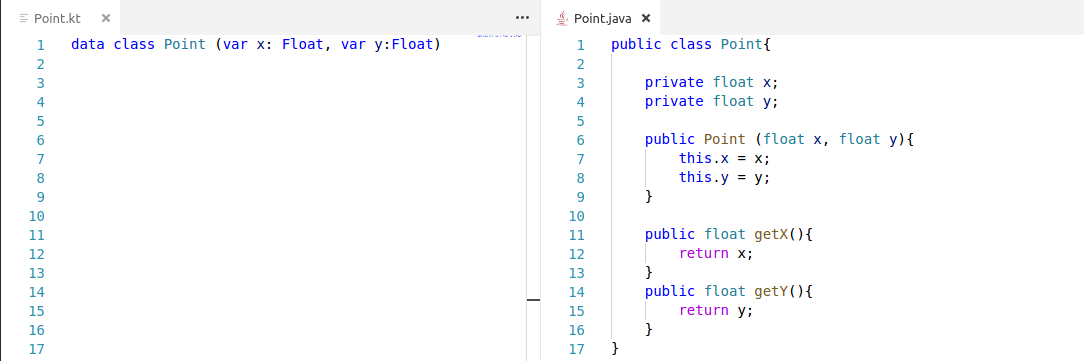
\includegraphics[scale=0.6]{images/kotlinexample}\\
\caption{\textit{Snippet} ejemplo de un \textit{POJO} Punto} A la izquierda, la versión en Java, a la derecha, la de Kotlin. Elaboración propia.
\end{figure}

Los motivos por los que se ha decidido utilizar Kotlin frente a Java son los siguientes \cite{kotlin}:
\begin{enumerate}

\item Permite una interoperabilidad completa con Java: al utilizar ambos la misma máquina virtual (y compilar en \textit{bytecode}), es posible la ejecución de métodos de Java en Kotlin y viceversa. De esta forma, permite integrar componentes desarrollados en un lenguaje desde el otro.

\item Es conciso: Kotlin elimina gran cantidad de \textit{“boilerplate“} en el código fuente. Por ejemplo, en el caso de una clase \textit{POJO}, los setters y los getters son generados en tiempo de compilación en el caso de que empleemos una clase de datos (\textit{data class)}.

\item Es \textit{“null-safe“}: Según el blog de programación \cite{tapikinull} \textit{Tapiki}, en un estudio realizado sobre 1.000 sistemas informáticos, un 70\% de ellos contenían errores de puntero nulo, que fue el motivo de excepción más frecuente. Kotlin intenta solucionar este problema forzando al programador a utilizar objetos que no pueden ser nulos, o bien, haciendo que tenga que indicar expresamente que un puntero puede ser nulo.

\item Por motivos académicos: En la asignatura \cite{smovkotlin} Sistemas Móviles del curso 2017-2018, impartida por D. Joaquín Adiego Rodríguez, se nos presentó esta tecnología y esto me motivó a querer utilizarla.

\item Por motivos de estándares: El apoyo que Google está dando al lenguaje de programación es tal que resulta más que recomendable empezar a utilizarlo y acostumbrarse al mismo.
\end{enumerate}

Por otro lado, también resulta de interés considerar las desventajas que suponen utilizar esta tecnología \cite{disadvKotlin}:
\begin{enumerate}

\item Curva de aprendizaje: Kotlin tiene características que no tiene Java y, por tanto, existe una cierta curva de aprendizaje que es necesario solventar.

\item Menor cantidad de documentación frente a Java: al ser un lenguaje tan nuevo, apenas se cuenta con una comunidad de desarrolladores, por lo que encontrar documentación concreta puede llegar a ser un problema.
\end{enumerate}

\subsection{Firebase}
\label{firebase}

\begin{figure}[H]
\centering

\includegraphics[scale=0.3]{images/firebase}\\
\caption{Logotipo de Firebase} \cite{firebase}
\end{figure}


Firebase es un producto de Google enmarcado dentro de su división \textit{Google Cloud}, plataforma del Gigante de Internet que ofrece recursos informáticos bajo demanda. Es utilizada para facilitar el desarrollo de aplicaciones Web y móviles, que posibilita la reducción del tiempo que se dedica a desarrollar áreas no específicas de la aplicación haciendo que el desarrollador pueda centrarse en aquello que la hará distinta. Fue creada en el año 2011 aunque en 2014 fue adquirida por Google.

Firebase ofrece un gran número de componentes ya desarrollados y listos para integrar, como las sesiones, las bases de datos, el alojamiento de archivos, las funciones, las estadísticas, etcétera.\\

Los motivos por los que se ha escogido Firebase son los siguientes \cite{firebaseadvdis}:

\begin{enumerate}

\item Facilita el desarrollo: los componentes que conforman el ecosistema Firebase ya se encuentran desarrollados y están listos para ser integrados en la aplicación. Estos son probados y utilizados por millones de usuarios todos los días y aplica los últimos estándares de seguridad informática.

\item \textit{Serverless} : en caso de no utilizar Firebase, el equipo de desarrollo tendría que preocuparse por los servidores y conexiones de red, intentando tener el máximo tiempo de \textit{uptime}, instalar actualizaciones, escalar  los recursos informáticos, asegurar la redundancia, etcétera.

\item Facilita la sincronización de los datos: Firebase está construido para que el usuario pueda trabajar sin conexión sobre la aplicación y actualizar los datos en cuanto tenga acceso a la red.
\end{enumerate}

Firebase también tiene una serie de desventajas:

\begin{enumerate}
\item Dependencia de una plataforma específica: Una vez se lanza una aplicación elaborada con Firebase es muy complicado cambiar de tecnología, puesto que deberemos añadir los costes de desarrollo de todos aquellos componentes que utilicen la plataforma.

\item Interfaces: Las interfaces de acceso a datos de Firebase no son muy flexibles y en algunos casos no podremos consultar directamente la información a la base de datos, sino que será necesario descargarla por completo para realizar las consultas en otra plataforma.

\end{enumerate}

En cuanto a las bases de datos de Firebase, se ha de destacar que ofrece en su paquete dos de tipo no relacional, \textit{Firebase Firestore} (basada en documentos) y \textit{Firebase Realtime} (basada en pares clave-valor). Para este trabajo se ha elegido la primera por varios motivos:

\begin{enumerate}
\item Mayor complejidad en las consultas: Firestore ofrece operaciones básicas de tipo \textit{WHERE}. Igualmente, ofrece los operadores \textit{ORDER BY} y \textit{LIMIT}.
\item Mayor escalabilidad: En Realtime cuando se accede a una parte del árbol (clave-valor), el usuario debe descargarse todos los hijos. En Firestore únicamente aquellos documentos que se deseen.
\item Mayor seguridad: Firestore ofrece mayores medidas de seguridad al tener reglas de lectura y escritura más complejas y flexibles.
\end{enumerate}

\section{Comunicación con el servidor}
La comunicación con el servidor es fundamental para el buen funcionamiento de la aplicación. En concreto, se deberá comunicar por los siguientes motivos:

\begin{itemize}
\item Realización de estadísticas: inicios y finalizaciones de una misión (para comprobar el éxito de las mismas), uso del usuario de la aplicación, etcétera.

\item Realización de misiones: las misiones de consumo y de reto social requieren una conexión a Internet para asegurarse de que el usuario haya completado el reto.

\item Descarga de nuevas misiones y niveles: uno de los requisitos del sistema informático en su conjunto es el de que el administrador pueda gestionar desde la parte Web los niveles y misiones, añadiéndolas y modificándolas bajo demanda.

\item Manteninimiento de un ranking global.

\item Conexión multidispositivo: se busca que el usuario pueda acceder a la aplicación desde distintos dispositivos, utilizando en todos ellos el sistema operativo Android.
\end{itemize}

Encontraremos dos tipos de conexiones:

\begin{itemize}
\item Conexiones realizadas a Firebase: datos estadísticos, de sesiones, invitaciones, base de datos, etcétera.

\item Conexiones realizadas para lanzar funciones de Firebase utilizando la autenticación de usuarios.

\end{itemize}


\chapter{Route66App}
\section{Plan de Desarrollo del Software}
\subsection{Descripción del proyecto}

La ludificación comenzó a popularizarse en 2010\cite{anatfg}, y desde entonces, tal y como he explicado en puntos anteriores de esta memoria, se ha aplicado en variados ámbitos (educación, ventas, proveedores, etcétera). En el caso que nos ocupa, un restaurante de comida americana, no podemos encontrar en España ningún ejemplo de una aplicación similar que aplique la ludificación.

Route66App consiste en una app para dispositivos móviles que aplica las ideas expuestas en el Trabajo Fin de Grado de una alumna del Grado en Organización Industrial \cite{cristinatfg}. Esta aplicación aplicará la teoría Bartle para identificar los diferentes tipos de jugador y buscará fidelizar y comprometer al usuario con los objetivos del negocio, por medio del juego.

Es importante destacar que este trabajo abarca solo una parte del proyecto completo, el cliente. Para su pleno funcionamiento se requerirá el gestor web, en el que se permitirá añadir y modificar las diferentes misiones que conforman el juego. 
 
\subsubsection{Propósito, objetivos y alcance}

El objetivo fundamental de  este trabajo es el de la implementación de un sistema de ludificación, aplicado a un restaurante de comida americana. En concreto se realizará la parte cliente, ejecutada desde terminales móviles con el Sistema Operativo Android.

La aplicación deberá contar con las siguientes funciones:
\begin{itemize}
\item Acciones propias del usuario
	\begin{itemize}
	\item Realizar misiones y juegos, con el fin de conseguir puntos y aumentar el nivel o posición en un ranking.
	\item Modificación del perfil del usuario, permitiendo actualizar el avatar del usuario.
	\item Consulta del historial de logros del usuario.
	\item Consulta de las insignias del usuario.
	\item Consulta del código QR que identifica al usuario de forma única.
	\item Consulta de la posición global del usuario (ranking).
	\end{itemize}
\item Acciones a realizar en grupo.
	\begin{itemize}
	\item Cosulta de los equipos a los que pertenece el usuario.
	\item Creación de nuevos equipos.
	\end{itemize}
\end{itemize}

Los objetivos serán:
\begin{itemize}
	\item Elaborar un sistema de usuarios, mediante el uso de sesiones.
	\item Gestionar un sistema de insignias, premios y logros (asignables tanto a equipos como a usuarios individuales). 
	\item Aumentar el compromiso del usuario con la aplicación, mediante el uso de juegos o misiones. Se busca que el usuario realice acciones correspondientes a los cuatro roles mencionados anteriormente.
	\item Hacer las funciones de una tarjeta de fidelización virtual, que permita al usuario identificarse a la hora de pagar.
\end{itemize}

\subsection{Metodología de Desarrollo del proyecto}
El proyecto aplicará el Proceso Unificado (\textit{Unified Process}), en concreto el proceso UPedu \cite{upedu}, cuyas caracterísiticas básicas \cite{pgpup} son: 
\begin{itemize}
\item Dirigido por los casos de uso.
\item Centrado en la arquitectura.
\item Iterativo e incremental
\end{itemize}
La iteratividad supone ciertas ventajas, como que se pueden mitigar los riesgos más críticos en las fases más tempranas o que permite obtener \textit{feedback} mucho antes, además, el aprendizaje obtenido se puede reaprovechar en etapas posteriores.

\subsection{Restricciones}
Se imponen las siguientes restricciones, extraídas tras una serie de entrevistas con la tutora del trabajo:

\begin{enumerate}
\item \textbf{Tiempo:} Este proyecto se realiza para cumplir con los objetivos de la asignatura Trabajo de Fin de Grado. Mención Ingeniería del Software, correspondiente a 12 créditos ECTS, unas 300 horas.

\item \textbf{Plazo mínimo de entrega:} Este proyecto se podrá entregar cuando haya terminado el resto de asignaturas de la Mención. Por tanto, hasta que no termine y tenga calificada la única asignatura que tendré en el segundo cuatrimestre (Prácticas en Empresa), no podrá ser entregado. Las prácticas curriculares en la empresa \textit{Telefónica Investigación y Desarrollo} concluyen el día 10 de Abril de 2018.

\item \textbf{Requisitos de la plataforma:} La aplicación será instalable en terminales Android, cuya versión de API sea igual o superior a la 19 (Android 4.4, KitKat). Según el sitio Web oficial de desarrolladores de Android \footnote{\url{https://developer.android.com/}}, esto supone cubrir la grandísima mayoría de los dispositivos (un 92.5 \%, a fecha 25 de Noviembre de 2017)\cite{androidversiondist}.

\item \textbf{Datos en el dispositivo}: la aplicación deberá contar con una caché de los datos en el dispositivo del cliente con el fin de reducir el número de peticiones que se hagan contra Firebase, así como para acelerar el funcionamiento de la aplicación en lugares con una baja conectividad.
\end{enumerate}

\subsection{Estructura organizativa}
\subsubsection{Estructura organizativa interna}
La estructura organizativa del proyecto estará formada por una única persona, que deberá ejercer cada uno de los roles en el momento en el que sea necesario. \cite{upedu} \vspace{0.5cm}

\begin{table}[H]
\begin{tabular}{llll}
\cline{1-2}
\multicolumn{1}{|c|}{Rol} & \multicolumn{1}{c|}{Encargado} &  &  \\ \cline{1-2}
\multicolumn{1}{|l|}{Desarrollador}                                      & \multicolumn{1}{l|}{Álvaro Carreras Regorigo}                                          &  &  \\ \cline{1-2}
\multicolumn{1}{|l|}{Analista}                                           & \multicolumn{1}{l|}{Álvaro Carreras Regorigo}                                          &  &  \\ \cline{1-2}
\multicolumn{1}{|l|}{Gestor de proyecto}                                 & \multicolumn{1}{l|}{Álvaro Carreras Regorigo}                                          &  &  \\ \cline{1-2}
\multicolumn{1}{|l|}{Diseñador}                                          & \multicolumn{1}{l|}{Álvaro Carreras Regorigo}                                                         &  &  \\ \cline{1-2}
                                                                         &                                                                               &  & 
\end{tabular}
\centering
\caption{Roles}
\end{table}
\vspace{0.5cm}

\paragraph{Desarrollador}\mbox{}\\

Este rol se encarga de implementar el código y de realizar las pruebas para los entregables software generados, con el fin de que sean integrados.

\paragraph{Analista}\mbox{}\\

Organiza y coordina tanto la elicitación de requisitos como el modelado de casos de uso indicando y limitando la funcionalidad del sistema y el alcance del mismo.

\paragraph{Gestor de Proyecto}\mbox{}\\

Realiza el control y mando del proyecto, asigna recursos, gestiona los reisgos, distribuye responsabilidades, gestiona la interacción con los clientes, etcétera.

\paragraph{Diseñador}\mbox{}\\

Como indica su nombre, está encargado de diseñar el sistema, definiendo las responsabilidades, operaciones y relaciones de cada uno de los componentes del sistema.

\subsubsection{Estructura organizativa externa}
Solo se identifica un rol en la estructura organizativa externa: el del usuario de la aplicación. 

\subsection{Gestión del proyecto}
\subsubsection{Planificación del proyecto}
En este proyecto se utilizará la metodología UPedu \cite{upedu}, compuesta por fases y estas por iteraciones.

\begin{figure}[h]
\label{upeduChart}
\begin{center}
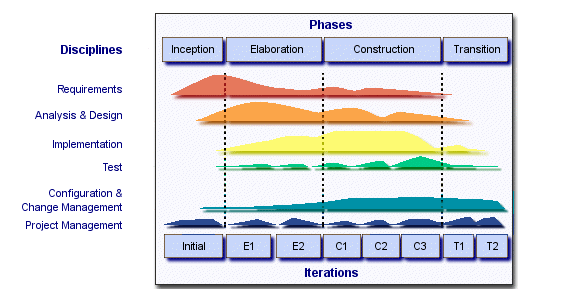
\includegraphics[scale=0.75]{images/upeduFases}
\caption{Fases de la metodología UPedu} \cite{upedu}
\end{center}
\end{figure}

En la figura \ref{upeduChart}, se puede observar el esfuerzo necesario de cada disciplina en cada fase del proyecto

\paragraph{Fase de inicio}\mbox{}\\

En esta fase no se realiza ningún artefacto de tipo software, pues estos se deben tratar antes de comenzar con la implementación. Los objetivos fundamentales de esta fase son la definición del alcance del proyecto,  la determinación de los casos de uso críticos, la estimación del coste y la duración del proyecto, y la elaboración de una primera gestión de riesgos.

\paragraph{Fase de elaboración}\mbox{}\\

El objetivo fundamental de esta fase \cite{pgpup} es el de la elaboración del diseño y arquitectura del sistema informático. Similarmente, se realizará un análisis del dominio del sistema y se eliminarán los elementos de mayor riesgo para el desarrollo del proyecto.

Después de esta fase, se obtendrá una arquitectura, requisitos y planes de desarrollo estables. Similarmente, se habrán reducido los riesgos más destacables.

\paragraph{Fase de construcción}\mbox{}\\

Es sin ninguna duda la parte más larga del proyecto y es la primera que tendrá como output entregables software utilizables.Se irá iterando y mejorando la calidad del producto software en cada ciclo.

La salida de esta fase \cite{pgpup} es software en estado beta.

\paragraph{Fase de transición}\mbox{}\\

Se deberá conseguir la aceptación por parte del usuario, indicando que cumple con la visión inicial del proyecto. Asímismo, se distribuirá el software.

\subsubsection{Calendario del proyecto}

Como se ha indicado en los apartados anteriores, este proyecto se ha dividido en las fases que el Proceso Unificado, en su variación UPedu\cite{upedu} establece. A continuación, se lista cada fase, el número de iteraciones y las horas de trabajo y duración estimadas. Estos cálculos son orientativos, las variaciones sobre los mismos están expuestas en el apartado correspondiente.

\begin{table}[H]
\centering
\begin{tabular}{|l|l|l|l|}
\hline
Nombre de la fase & Núm.. Iteraciones & Horas de trabajo & Duración estimada \\ \hline
Inicio            & 1                 & 10 horas/semana  & 61 horas       \\ \hline
Elaboración       & 2                 & 20 horas/semana  & 80 horas    \\ \hline
Construcción      & 2                 & 20 horas/semana  & 108 horas       \\ \hline
Transición        & 1                 & 20 horas/semana   & 42 horas       \\ \hline
\end{tabular}
\caption{Fases del proceso UPedu}
\end{table}

La duración estimada total es de 316 horas, a lo que habría que añadir las necesarias para acudir a las tutorías.

\paragraph{Fase de inicio}\mbox{}\\

Comienza el día 6 de Noviembre de 2017 y finaliza el 10 de Diciembre de 2017. Consta de una única iteración. Solo trabajaré en el T.F.G. durante los viernes y fines de semana.

\begin{figure}[h]
\begin{center}
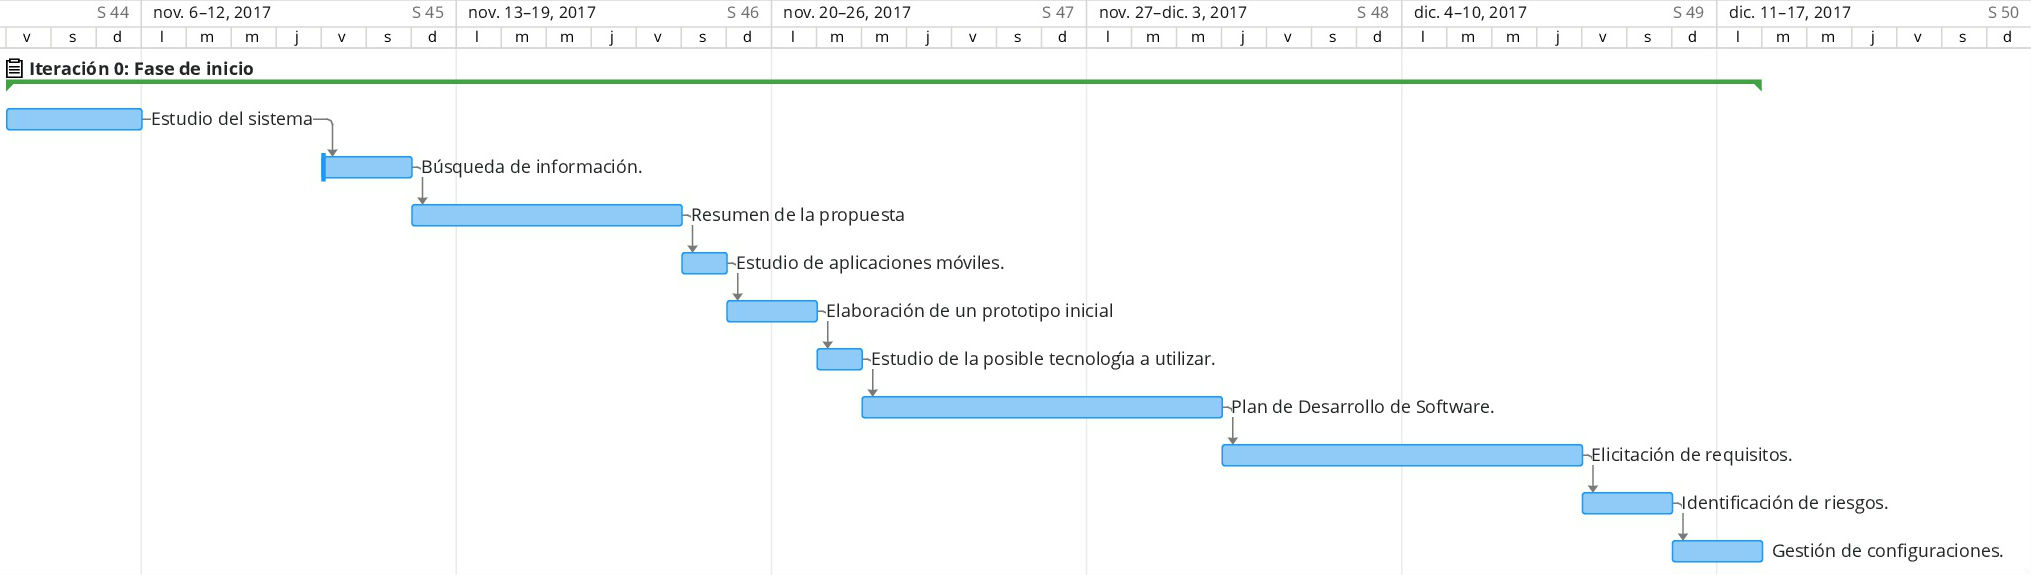
\includegraphics[height=9cm, width=\textwidth]{images/gantt/ite0}
\caption{Diagrama de Gantt para la iteración 0 (fase de inicio)}
\end{center}
\end{figure}

\begin{table}[H]
\centering
	\begin{tabular}{|l|l|l|l|}
    \hline
    Nombre de la tarea                           & Fecha de comienzo & Fecha de fin & Duración \\ \hline
    Estudio del sistema.                         & 03/11/2017        & 05/11/2017   & 10 horas  \\ \hline
    Búsqueda de información.                     & 10/11/2017        & 11/11/2017   & 4 horas   \\ \hline
    Resumen de la propuesta                      & 11/11/2017        & 17/11/2017   & 6 horas   \\ \hline
    Estudio de aplicaciones móviles.             & 17/11/2017        & 17/11/2017   & 2 horas   \\ \hline
    Elaboración de un prototipo inicial          & 18/11/2017        & 19/11/2017   & 7 horas   \\ \hline
    Estudio de la posible tecnología a utilizar. & 19/11/2017        & 19/11/2017   & 3 horas   \\ \hline
    Plan de Desarrollo de Software.              & 24/11/2017        & 01/12/2017   & 13 horas   \\ \hline
    Elicitación de requisitos.                   & 01/12/2017        & 08/12/2017   & 12 horas   \\ \hline
    Identificación de riesgos.                   & 08/12/2017        & 09/12/2017   & 3 horas   \\ \hline
    Gestión de configuraciones.                  & 09/12/2017        & 10/12/2017   & 1 horas   \\ \hline
    \end{tabular}
    \caption{Iteración 0. Fase de Inicio.}
\end{table}

Reuniones realizadas con la tutora del T.F.G.:

\begin{itemize}
\item 30 de Octubre de 2017.
\item 6 de Noviembre de 2017.
\item 20 de Noviembre de 2017.
\item 4 de Diciembre de 2017.
\end{itemize}

\paragraph{Fase de elaboración}\mbox{}\\

Se ha decidido dejar un lapso temporal de 41 días (10 de Diciembre - 20 Enero) por la gran acumulación de trabajos y exámenes.

Esta fase comienza el día 20 de Enero de 2017 y finaliza el 1 de Marzo de 2018. Consta de dos iteraciones.

\begin{itemize}
\item Iteración 1: Con una duración de 3 semanas.
\item Iteración 2: Con una duración de 1 semana y media.
\end{itemize}

\begin{figure}[h]
\begin{center}
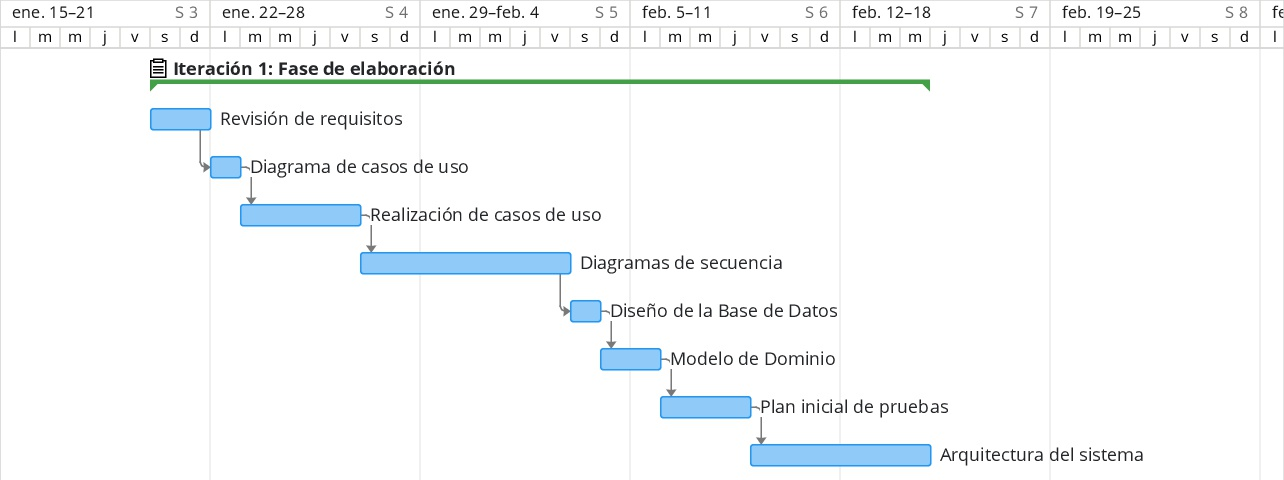
\includegraphics[width=\textwidth]{images/gantt/ite1}
\caption{Diagrama de Gantt para la iteración 1 (fase de elaboración)}
\end{center}
\end{figure}

\begin{table}[H]
\centering
\begin{tabular}{|l|l|l|l|}
\hline
Nombre de la tarea          & Fecha de comienzo & Fecha de fin & Duración \\ \hline
Revisión de requisitos      & 20/01/2018        & 21/01/2018   & 5 horas   \\ \hline
Diagrama de casos de uso    & 22/01/2018        & 22/01/2018   & 1 hora   \\ \hline
Realización de casos de uso & 22/01/2018        & 25/01/2018   & 10 horas  \\ \hline
Diagramas de secuencia      & 26/01/2018        & 01/02/2018   & 20 horas  \\ \hline
Modelo de Dominio 			& 02/02/2018        & 03/02/2018   & 5 horas    \\ \hline
Diseño de la Base de Datos  & 02/02/2018        & 02/02/2018   & 3 horas   \\ \hline
Plan inicial de pruebas     & 03/02/2018        & 05/02/2018   & 5 horas   \\ \hline
Arquitectura del sistema    & 05/02/2018        & 10/02/2018   & 13 horas   \\ \hline
\end{tabular}
\caption{Iteración 1. Fase de elaboración.}
\end{table}

Reuniones realizadas con la tutora del T.F.G.:
\begin{itemize}
\item 6 de Febrero de 2018.
\end{itemize}


\begin{figure}[h]
\begin{center}
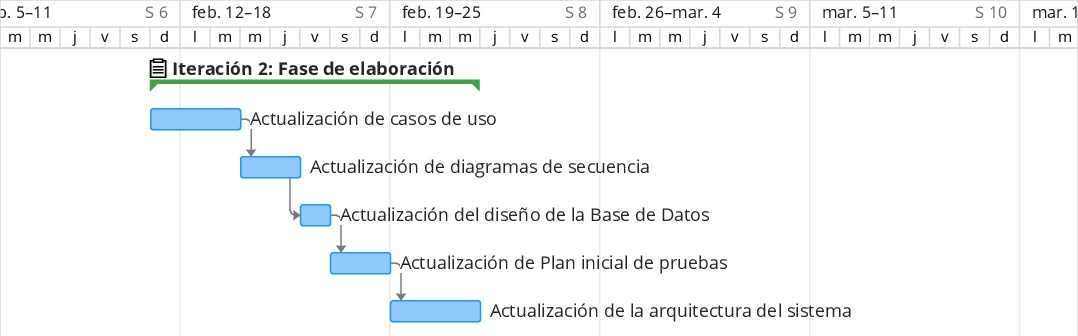
\includegraphics[width=\textwidth]{images/gantt/ite2}
\caption{Diagrama de Gantt para la iteración 2 (fase de elaboración)}
\end{center}
\end{figure}


\begin{table}[H]
\centering
\begin{tabular}{|l|l|l|l|}
\hline
Nombre de la tarea                           & Fecha de comienzo & Fecha de fin & Duración \\ \hline
Actualización de casos de uso                & 11/02/2018        & 13/02/2018   & 5 horas   \\ \hline
Actualización de diagramas de secuencia      & 14/02/2018        & 15/02/2018   & 4 horas   \\ \hline
Actualización del diseño de la Base de Datos & 16/02/2018        & 16/02/2018   & 2 horas   \\ \hline
Actualización de Plan inicial de pruebas     & 17/02/2018        & 18/02/2018   & 2 horas   \\ \hline
Actualización de la arquitectura del sistema & 18/02/2018        & 20/02/2018   & 5 horas   \\ \hline
\end{tabular}
\caption{Iteración 2. Fase de elaboración.}
\end{table}

El día 20 de Febrero se hace entrega a la tutora de todos los entregables realizados hasta la fecha, con el fin de que puedan ser revisados y validados en profundidad.


\paragraph{Fase de construcción}\mbox{}\\

Comienza el día 1 de Marzo de 2018 y finaliza el 16 de Abril de 2018.

\begin{figure}[h]
\begin{center}
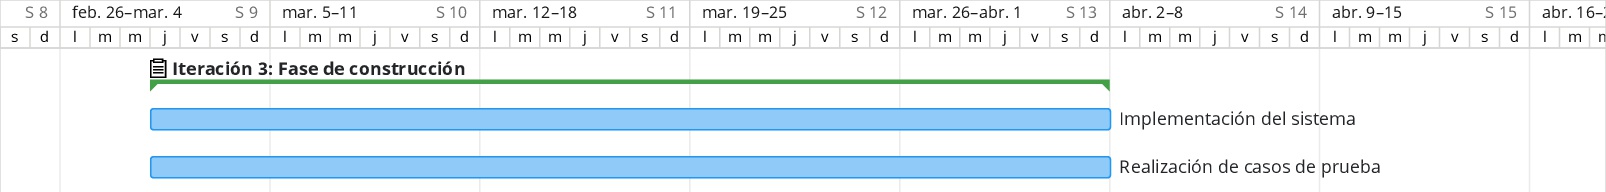
\includegraphics[height=3cm,width=\textwidth]{images/gantt/ite3}
\caption{Diagrama de Gantt para la iteración 3 (fase de construcción)}
\end{center}
\end{figure}


\begin{table}[H]
\centering
\begin{tabular}{|l|l|l|l|}
\hline
Nombre de la tarea             & Fecha de comienzo & Fecha de fin & Duración \\ \hline
Implementación del sistema & \multirow{2}{*}{01/03/2018}  & \multirow{2}{*}{01/04/2018}   & \multirow{2}{*}{91 horas}  \\
Realización de casos de prueba & & & \\
\hline
\end{tabular}
\caption{Iteración 3. Fase de construcción.}
\end{table}

En la iteración 3 (Fase de construcción) se ha estipulado la misma duración y mismas fechas a ambas tareas porque se planea implementar e inmediatamente probar.

Reuniones realizadas con la tutora del T.F.G.:
\begin{itemize}
\item 6 de Marzo de 2018.
\item 20 de Marzo de 2018.
\end{itemize}


\begin{figure}[h]
\begin{center}
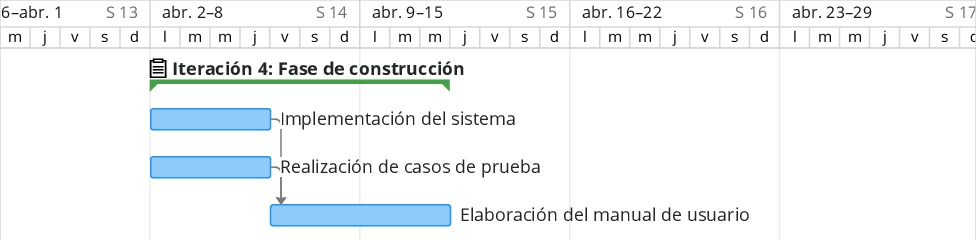
\includegraphics[width=\textwidth]{images/gantt/ite4}
\caption{Diagrama de Gantt para la iteración 4 (fase de construcción)}
\end{center}
\end{figure}

\begin{table}[H]
\centering
\begin{tabular}{|l|l|l|l|}
\hline
Nombre de la tarea                & Fecha de comienzo & Fecha de fin & Duración \\ \hline
Implementación del sistema        & \multirow{2}{*}{02/04/2018} & \multirow{2}{*}{05/04/2018}   & \multirow{2}{*}{7 horas}  \\
Realización de casos de prueba    & &   &   \\ \hline
Elaboración del manual de usuario & 05/04/2018        & 10/04/2018   & 10 horas   \\ \hline

\end{tabular}
\caption{Iteración 4. Fase de construcción.}
\end{table}

\paragraph{Fase de transición}\mbox{}\\

Comienza el día 16 de Abril de 2018 y finaliza el 30 de Abril de 2018.

\begin{figure}[h]
\begin{center}
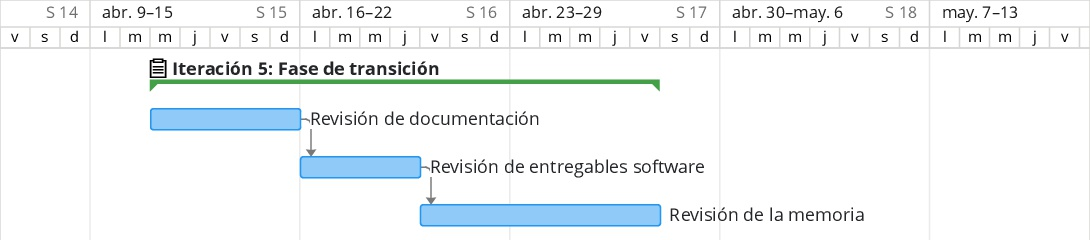
\includegraphics[width=\textwidth]{images/gantt/ite5}
\caption{Diagrama de Gantt para la iteración 5 (fase de transición)}
\end{center}
\end{figure}


\begin{table}[H]
\centering
\begin{tabular}{|l|l|l|l|}
\hline
Nombre de la tarea              & Fecha de comienzo & Fecha de fin & Duración \\ \hline
Revisión de documentación       & 11/04/2018        & 15/04/2018   & 12 horas   \\ \hline
Revisión de entregables software & 15/04/2018        & 18/04/2018   & 9 horas   \\ \hline
Revisión de la memoria & 18/04/2018        & 25/04/2018   & 21 horas   \\ \hline
\end{tabular}
\caption{Iteración 5. Fase de transición.}
\end{table}

\subsection{Relación de entregables no software}

Los distintos entregables a realizar son los siguientes. En todo caso, siempre se considerará como definitiva la versión final de los documentos entregados.
\paragraph{Fase de inicio\\}
\begin{itemize}
\item Plan de Desarrollo de Software.
\item Versión inicial del Plan de Gestión de Riesgos.
\end{itemize}
\paragraph{Fase de elaboración\\}
\begin{itemize}
\item Documento de requisitos \textit{software}.
\item Versión inicial de los Casos de Uso.
\item Diagramas de secuencia.
\item Arquitectura del sistema.
\item Diseño de la Base de Datos.
\item Elaboración de prototipos.
\end{itemize}

\paragraph{Fase de construcción\\}
\begin{itemize}
\item Versión inicial del manual de usuario.
\item Documento de casos de prueba.
\item Documento de resultados de las pruebas.
\end{itemize}

\paragraph{Fase de transición\\}
\begin{itemize}
\item Versión final del manual de instalación.
\item Versión final del manual de usuario.
\end{itemize}

\subsection{Control y seguimiento del proyecto.}

Se hará un control y seguimiento del proyecto en todo momento, utilizando la herramienta Asana \footnote{\url{https://app.asana.com}}, tal y como se ha expuesto en el apartado “Herramientas utilizadas“.

El control y seguimiento del proyecto resulta ser una tarea fundamental para asegurar el buen progreso del proyecto y asegurar el cumplimiento de los objetivos marcados, en especial en cuanto al cumplimiento de los hitos establecidos, ya que el gestor del proyecto podrá observar las distintas variaciones de tiempo programadas versus reales para así poder reaccionar y poder tomar las medidas que sean precisas para ajustarse al cronograma del proyecto.

\subsection{Gestión de riesgos.}

Se identifican los siguientes riesgos:

\begin{risk}
  \addheading{R0}{Falta de experiencia del alumno}
  \addrow{Descripción}{El alumno ha realizado prácticas en Android, pero puede encontrarse en momentos en los que requiera experiencia adicional.}
  \addrow{Consecuencia}{Ralentización del trabajo.}
  \addrow{Probabilidad}{Media.}
  \addrow{Impacto}{Bajo.}
  \addrow{Estrategia}{Reservar el riesgo}
  \addrow{Plan de acción}{Buscar información y ayuda, ya sea preguntando a la tutora del trabajo o utilizando otros medios.}
  \addrow{Plan de contingencia}{Revisión de conocimientos existentes.}
\end{risk}

\vspace{0.5cm}

\begin{risk}
  \addheading{R1}{Retraso en la planificación}
  \addrow{Descripción}{Debido a errores en la estimación, la planificación no se ajusta a la realidad y se producen demoras en las fechas de entrega.}
  \addrow{Consecuencia}{Retraso en la entrega de los entregables.}
  \addrow{Probabilidad}{Alta }
  \addrow{Impacto}{Crítico}
  \addrow{Estrategia}{Reservar el riesgo}
  \addrow{Plan de acción}{Realizar una nueva planificación más realista. }
  \addrow{Plan de contingencia}{Realizar revisiones periódicas del calendario de planificación.}
\end{risk}

\vspace{0.5cm}

\begin{risk}
  \addheading{R2}{Adelantos en la planificación}
  \addrow{Descripción}{Debido a errores en la estimación, la planificación no se ajusta a la realidad y se producen adelantos en las fechas de entrega.}
  \addrow{Consecuencia}{Modificación de toda la planificación.}
  \addrow{Probabilidad}{Alta }
  \addrow{Impacto}{Crítico}
  \addrow{Estrategia}{Reservar el riesgo}
  \addrow{Plan de acción}{Realizar una nueva planificación más realista. }
  \addrow{Plan de contingencia}{Realizar revisiones periódicas del calendario de planificación.}
\end{risk}

\vspace{0.5cm}

\begin{risk}
  \addheading{R3}{Falta de experiencia en grandes proyectos.}
  \addrow{Descripción}{El equipo no cuenta con experiencia propia de proyectos de gran extensión que le permita calcular mejor las estimaciones, así como realizar el proyecto con mayor celeridad.}
  \addrow{Consecuencia}{Peor organización y estimaciones. Grandes picos de trabajo.}
  \addrow{Probabilidad}{Alta }
  \addrow{Impacto}{Alto. }
  \addrow{Estrategia}{Reducción del riesgo.}
  \addrow{Plan de acción}{Realizar una nueva planificación. }
  \addrow{Plan de contingencia}{Realizar revisiones periódicas del calendario de planificación.}
\end{risk}

\vspace{0.5cm}

\begin{risk}
  \addheading{R4}{Falta de disponibilidad}
  \addrow{Descripción}{El alumno no puede continuar con el trabajo por falta de disponibilidad.}
  \addrow{Consecuencia}{Dependerá del tiempo en el que esté no disponible y las holguras en la planificación. Si es muy largo, puede suponer la no entrega del trabajo a tiempo.}
  \addrow{Probabilidad}{Baja.}
  \addrow{Impacto}{Crítico. }
  \addrow{Estrategia}{Reservar del riesgo.}
  \addrow{Plan de acción}{Realizar una nueva planificación basándose en las nuevas fechas \\de disponibilidad.}
  \addrow{Plan de contingencia}{Monitorizar la disponibilidad del alumno.}
\end{risk}

\vspace{0.5cm}

\begin{risk}
  \addheading{R5}{Pérdida de datos}
  \addrow{Descripción}{Por cualquier motivo, se pierde total o parcialmente cualquiera de los entregables ya realizados o en proceso de realización.}
  \addrow{Consecuencia}{Ralentización muy alta del trabajo. Repetición de los entregables perdidos. }
  \addrow{Probabilidad}{Bajo.}
  \addrow{Impacto}{Crítico. }
  \addrow{Estrategia}{Evitación del riesgo.}
  \addrow{Plan de acción}{No se aplica}
  \addrow{Plan de contingencia}{Realización de copias de seguridad y uso de un sistema de control de versiones (ver apartado gestión de configuraciones)}
\end{risk}

\vspace{0.5cm}

\begin{risk}
  \addheading{R6}{Falta de medios software de desarrollo}
  \addrow{Descripción}{Las herramientas designadas para desarrollar el proyecto fallan, desaparecen o dejan de estar disponibles.}
  \addrow{Consecuencia}{Ralentización muy alta del trabajo. Repetición de los entregables perdidos. }
  \addrow{Probabilidad}{Bajo.}
  \addrow{Impacto}{Crítico. }
  \addrow{Estrategia}{Evitación del riesgo.}
  \addrow{Plan de acción}{No se aplica}
  \addrow{Plan de contingencia}{Utilización de herramientas profesionales, aplicación de las últimas actualizaciones.}
\end{risk}

\vspace{0.5cm}

\begin{risk}
  \addheading{R7}{Falta de medios hardware de desarrollo}
  \addrow{Descripción}{Las herramientas designadas para desarrollar el proyecto fallan o dejan de estar disponibles.}
  \addrow{Consecuencia}{Adquisición de nuevos materiales.}
  \addrow{Probabilidad}{Bajo.}
  \addrow{Impacto}{Alto. }
  \addrow{Estrategia}{Evitación del riesgo.}
  \addrow{Plan de acción}{No se aplica}
  \addrow{Plan de contingencia}{Realización de copias de seguridad de los entregables, para evitar su pérdida en caso de ocurrir este riesgo.}
\end{risk}

\vspace{0.5cm}

\begin{risk}
  \addheading{R8}{Diseño pobre o incorrecto.} 
  \addrow{Descripción}{El diseño realizado del sistema es pobre o incorrecto.}
  \addrow{Consecuencia}{Ralentización del trabajo.}
  \addrow{Probabilidad}{Medio.}
  \addrow{Impacto}{Crítico. }
  \addrow{Estrategia}{Reducción del riesgo.}
  \addrow{Plan de acción}{Rediseñar la arquitectura del sistema.}
  \addrow{Plan de contingencia}{Realizar revisiones con el cliente y realizar pruebas sobre el modelo diseñado.}
\end{risk}

\subsection{Gestión de configuraciones.}

Hoy en día, la mayoría de los servicios públicos que ofrecen alojamiento de repositorios Git permiten realizar una buena gestión de configuraciones. Esto es debido a que cada cambio que se hace sobre el código fuente (\textit{commit}) viene asociado a informaciones sobre qué se ha cambiado, quién lo ha cambiado, cuándo lo ha cambiado, etcétera. Además, las ramas o \textit{branches}, aquellos lugares donde van dirigidos los cambios, permiten imponer bloqueos sobre escritura a ciertos usuarios, con el fin de proteger los entregables que estuvieran en la misma.

Por otro lado, estos servicios también pueden ser utilizados para la gestión de \textit{releases}. Esto se puede llevar a cabo mediante la creación de una rama específica para ese propósito o, directamente, y si se permite, mediante el apartado correspondiente desde el sitio web.

En el caso de este proyecto se han utilizado dos repositorios privados en \textit{GitHub}\footnote{\url{https://github.com/}}, en uno de ellos se tratará el desarrollo de esta memoria y en otro, el del código del sistema informático que se desea construir.

\subsection{Estimación de los costes.}

Para una correcta estimación de los costes se debe procurar partir de datos de proyectos reales, que nos permita realizarla partiendo de una experiencia. Desafortunadamente, como estos no se hacen públicos (pues son parte de la estrategia de la empresa), no es posible contar con ellos. Por este motivo, he realizado los cálculos basándome en lo que he estudiado en la asignatura \cite{pgptema2} Planificación y Gestión de Proyectos, así como aquella información que he encontrado por Internet.

El resultado de la estimación total de costes es de \textbf{12.459,96\euro}, que se detallarán a continuación.

\subsubsection{Costes \textit{hardware} y \textit{software}}
\textbf{Costes \textit{hardware}}
\begin{table}[H]
\center
\begin{tabular}{|l|l|l|l|l|}
\hline
Dispositivo        & Coste de compra   & Horas dispositivo & Horas utilizadas & Coste total \\ \hline
Teléfono Android   & 120 \euro      & 17.520 horas (2 años, 24 horas diarias)  & 133  & 0,92  \euro \\ \hline
Portátil      & 399 \euro   &  11.680 horas (4 años, 8 horas diarias) & 300 horas  & 10,25 \euro \\ \hline
\end{tabular}
\caption{Costes de los recursos \textit{hardware}}
\end{table}

Coste total del \textit{hardware} es: \textbf{11,16 \euro}.

Los costes de software, son, en realidad, 0 \euro, ya que se ha priorizado utilizar software gratuito (\textit{freeware}) y,  en los casos en los que se ha decidido usar uno privativo, se han empleado licencias gratuitas para estudiantes. Se ha de tener presente que estos son cálculos que sí se aplicarían en un proyecto real que tenga como fin un beneficio económico.

\begin{table}[H]
\centering
\begin{tabular}{|l|l|l|}
\hline
Servicio         & Coste mensual & Coste total \\ \hline
GitHub Developer & 5,90 \euro        & 47,20 \euro          \\ \hline
Firebase         & 21 \euro      & 168\euro           \\ \hline
Astah Professional & 7,50 \euro & 60 \euro \\ \hline
\end{tabular}
\caption{Costes de los recursos \textit{software}}
\end{table}

Coste total de software: \textbf{240,80 \euro}.

Los datos anteriores se han calculado basándose en los datos públicos de las herramientas, convertido a euros según la tasa de cambio del 28 de Noviembre de 2017, para un período de 7 meses (Noviembre-Mayo).

El resto de \textit{software} utilizado (sistema operativo, \textit{IDE}, etcétera) es de licencia gratuita. No se ha empleado software cuya licencia solo fuera gratuita en casos de uso no comercial del mismo.

Coste total de este apartado: \textbf{251,96 \euro}.

\subsubsection{Costes de dietas, viajes y aprendizajes}

Los costes de dietas y de aprendizajes no se aplican en este apartado porque, en primer lugar, no se hará ninguna dieta externa y, en segundo lugar, se aplicarán los conocimientos adquiridos a lo largo del Grado, así como otros externos que se han adquirido en los tiempos libres, pero fuera del tiempo de asignación del proyecto.

Los viajes a estimar son aquellos que serían precisos realizar para poder realizar reuniones con la persona que ha encargado el proyecto (la tutora del mismo). Debido a que mi residencia habitual está en Laguna de Duero y utilizando la herramienta de mapas \textit{Vía Michelín}\footnote{\url{https://www.viamichelin.es}}, basándose en un coche urbano de diésel, los costes de viajes y transportes son:

\begin{itemize}
\item \textbf{Kilómetros recorridos por viaje:} 33 (16,5 por trayecto).
\item \textbf{Coste por viaje:} 3 \euro \hspace{0.1cm} (1,50 \euro \hspace{0.1cm} por trayecto).
\item \textbf{Viajes realizados:} 10.
\item \textbf{Coste total viajes:} 30 \euro.
\end{itemize}

Por tanto, el coste total de este apartado es: \textbf{30\euro}.

\subsubsection{Coste del esfuerzo (recursos humanos y seguros sociales)}

Para el caso de los primeros, los costes de los recursos humanos, debemos ver el listado de roles que se van a practicar a lo largo del proyecto:

\begin{table}[H]
\center
\begin{tabular}{|l|l|l|l|l|l|}
\hline
Rol                & Salario medio & \euro/Hora   & Horas estimadas & Coste total \\ \hline
Analista           & 59.615 \euro      & 31,05 \euro & \multirow{5}{*}{300 horas} & \multirow{5}{*}{9.315 \euro} \\\cline{1-3}
Desarrollador      & 59.615 \euro      & 31,05 \euro  & & \\\cline{1-3}
Gestor de proyecto & 59.615 \euro      & 31,05 \euro & & \\ \cline{1-3}
Diseñador          & 59.615 \euro      & 31,05 \euro & & \\ \cline{1-3}
Director de proyecto & 59.615 \euro    & 31,05 \euro & & \\ \cline{1-3}
\hline
\end{tabular}
\caption{Costes de los Recursos Humanos}
\end{table}

Los datos de la tabla anterior han sido calculados basándose en los datos de \cite{infojobs2016} Informe Anual Infojobs 2016 España (salario promedio bruto anual de un director de proyectos informático). Se ha dividido la cantidad anterior en doce pagas y veinte días de trabajo por mes.

Similarmente, también habría que considerar el coste de los seguros sociales. Como la estimación del proyecto se ha realizado  habiendo un único empleado, en régimen de autónomo, se aplicaría, por tanto, el coste de las cuotas que establece el Régimen Especial de Autónomos, que en 2018 es de 50 \euro \vspace{0.1cm} al mes para nuevos autónomos menores de 30 años \cite{segsocialautonomos}.

\begin{itemize}
\item Cuota mensual autónomos.
	\begin{itemize}
	\item \textbf{Importe mensual:} 50 \euro.
	\item \textbf{Número de cuotas (meses): } 7.
	\item \textbf{Importe total: } 350 \euro.
	\end{itemize}
\end{itemize}

El coste total de este apartado es de \textbf{9.715 \euro}.

\subsubsection{Costes indirectos aplicados al personal del proyecto}

Los costes indirectos son aquellos derivados del uso de calefacción, electricidad, comunicaciones, etcétera.

\begin{itemize}

\item Alquiler: se utilizará el servicio de vivero de empresas que propone el \cite{pcuva} Parque Científico de la Universidad de Valladolid para una sala de 23 ${m}^{2}$.
	\begin{itemize}
		\item \textbf{Coste estimado (mensual): } 276 \euro.
		\item \textbf{Número de meses:} 7.
		\item \textbf{Coste total:} 1.932\euro.
	\end{itemize}
	
\item Conexión a Internet y llamadas \textit{(Movistar Fibra óptica 300 MB)}:
	\begin{itemize}
		\item \textbf{Coste estimado (mensual):} 45 \euro \hspace{0.1cm}al mes + 19.99 \euro \hspace{0.1cm} al mes por la cuota de línea. Total: 65 \euro \hspace{0.1cm} al mes.
		\item \textbf{Número de meses:} 7.
		\item \textbf{Coste total:} 455 \euro.
	\end{itemize}
		
\item Telefonía móvil \textit{(Simyo 4GB + llamadas ilimitadas)}:
	\begin{itemize}
		\item \textbf{Coste estimado (mensual):} 18 \euro \hspace{0.1cm} al mes.
		\item \textbf{Número de meses:} 7.
		\item \textbf{Coste total:} 126 \euro.
	\end{itemize}

\end{itemize}

El coste total de este apartado es de \textbf{2.513 \euro}.

\subsection{Desviaciones sobre el calendario planificado}

Se adjunta a continuación la tabla de estimaciones de planificación, así como los retrasos que ha habido en realidad.

\begin{table}[H]
\centering
\resizebox{\textwidth}{!}{%
\begin{tabular}{|l|l|l|l|l|l|l|}
\hline
Iteración & Etapa        & Fecha de inicio real & Fecha inicio estimada & Fecha de fin real & Fecha fin estimada & Diferencia finalización \\ \hline
0         & Inicio       & 03/11/2017           & 06/11/2017            & 12/12/2017        & 10/12/2017         & 2 días                  \\ \hline
1         & Elaboración  & 20/01/2018           & 20/01/2018            & 15/02/2018        & 10/02/2018         & 5 días                  \\ \hline
2         & Elaboración  & 16/02/2018           & 11/02/2018            & 23/02/2018        & 20/02/2018         & 3 días                 \\ \hline
3         & Construcción & 24/02/2018           & 20/02/2018            & 03/04/2018        & 01/04/2018         &            2 días\\ \hline
4         & Construcción &                      & 02/04/2018            &                   & 10/04/2018         &                         \\ \hline
5         & Transición   &                      & 11/04/2018            &                   & 25/04/2018         &                         \\ \hline
\end{tabular}%
}
\caption{Desviaciones sobre el calendario planificado}
\end{table}

Tras un análisis de los retrasos sobre la planificación establecida se extraen las siguientes conclusiones:
\begin{itemize}

\item La planificación ha estado bastante ajustada a las estimaciones realizadas, encontrándose una mayor desviación en la iteración 1, correspondiente a la fase de elaboración. El motivo fue que se tuvo que compaginar el comienzo de las prácticas (y formación adicional) junto con el T.F.G., por lo que durante esos días no pude contar con el número de horas especificadas.

\item En la primera fase de construcción, hubo dos días en los que no pude trabajar porque decidí adquirir ampliar la memoria del ordenador, así como sustituir el disco duro por uno de estado sólido (SSD) con el fin de aumentar la productividad en esta fase. En esos días me dediqué a instalar esos dos componentes, así como los elementos software requeridos para la continuación del trabajo.

\end{itemize}


\section{Análisis}
\subsection{Requisitos}

\newcounter{functionalRequirements}
\subsubsection{Requisitos funcionales}

\textbf{Relacionados con los usuarios}\\

\begin{req}
	\addheading{\textbf{RF\arabic{functionalRequirements}}}{Sesiones}
	\addrow{Descripción}{El sistema permitirá iniciar sesión}
\end{req} \\\stepcounter{functionalRequirements}
 
\begin{req}
	\addheading{\textbf{RF\arabic{functionalRequirements}}}{Registro e inicio de sesión rápido.}
	\addrow{Descripción}{El sistema permitirá iniciar sesión y registrarse mediante el uso de servicios de terceros.}
\end{req} \\\stepcounter{functionalRequirements}

\begin{req}
	\addheading{\textbf{RF\arabic{functionalRequirements}}}{Registro de usuarios}
	\addrow{Descripción}{El sistema permitirá registrar usuarios}
\end{req}\\\stepcounter{functionalRequirements}

\begin{req}
	\addheading{\textbf{RF\arabic{functionalRequirements}}}{Configuración del usuario}
	\addrow{Descripción}{El sistema permitirá editar la configuración del usuario}
\end{req}\\\stepcounter{functionalRequirements}

\begin{req}
	\addheading{\textbf{RF\arabic{functionalRequirements}}}{Ranking de usuarios}
	\addrow{Descripción}{El sistema permitirá ver el ranking de usuarios}
\end{req}\\\stepcounter{functionalRequirements}

\begin{req}
	\addheading{\textbf{RF\arabic{functionalRequirements}}}{Invitación de usuarios a la aplicación.}
	\addrow{Descripción}{El sistema permitirá invitar a usuarios a la aplicación.}
\end{req}\\\stepcounter{functionalRequirements}

\begin{req}
	\addheading{\textbf{RF\arabic{functionalRequirements}}}{Avatares.}
	\addrow{Descripción}{El sistema permitirá añadir una fotografía de perfil (avatar) al usuario}
\end{req}\\\stepcounter{functionalRequirements}

\begin{req}
	\addheading{\textbf{RF\arabic{functionalRequirements}}}{Logros.}
	\addrow{Descripción}{El sistema permitirá consultar los logros de un usuario}
\end{req}\\\stepcounter{functionalRequirements}

\begin{req}
	\addheading{\textbf{RF\arabic{functionalRequirements}}}{Insignias.}
	\addrow{Descripción}{El sistema permitirá consultar las insignias que tiene un usuario}
\end{req}\\\stepcounter{functionalRequirements}

\begin{req}
	\addheading{\textbf{RF\arabic{functionalRequirements}}}{Código QR.}
	\addrow{Descripción}{El sistema permitirá mostrar el código QR asociado a una misión de tipo consumo.}
\end{req}\\\stepcounter{functionalRequirements}

\begin{req}
	\addheading{\textbf{RF\arabic{functionalRequirements}}}{Progreso del usuario}
	\addrow{Descripción}{El sistema permitirá mostrar el círculo de progresos relativo a cada usuario.}
\end{req}\\\stepcounter{functionalRequirements}

\begin{req}
	\addheading{\textbf{RF\arabic{functionalRequirements}}}{Identificación de usuarios}
	\addrow{Descripción}{El sistema permitirá identificar usuarios por correo electrónico o número de teléfono.}
\end{req}\\\stepcounter{functionalRequirements}


\begin{req}
	\addheading{\textbf{RF\arabic{functionalRequirements}}}{Premios.}
	\addrow{Descripción}{El sistema permitirá conceder premios a los usuarios.}
\end{req}\\\stepcounter{functionalRequirements}

\textbf{Relacionados con los grupos}\\

\begin{req}
	\addheading{\textbf{RF\arabic{functionalRequirements}}}{Creación de un grupo}
	\addrow{Descripción}{El sistema permitirá crear un grupo}
\end{req}\\\stepcounter{functionalRequirements}

\begin{req}
	\addheading{\textbf{RF\arabic{functionalRequirements}}}{Eliminación de un grupo}
	\addrow{Descripción}{El sistema permitirá eliminar un grupo}
\end{req}\\\stepcounter{functionalRequirements}

\begin{req}
	\addheading{\textbf{RF\arabic{functionalRequirements}}}{Unirse a un grupo}
	\addrow{Descripción}{El sistema permitirá unirse a un grupo}
\end{req}\\\stepcounter{functionalRequirements}

\begin{req}
	\addheading{\textbf{RF\arabic{functionalRequirements}}}{Salirse de un grupo}
	\addrow{Descripción}{El sistema permitirá salirse de un grupo}
\end{req}\\\stepcounter{functionalRequirements}

\begin{req}
	\addheading{\textbf{RF\arabic{functionalRequirements}}}{Expulsión de un grupo}
	\addrow{Descripción}{El sistema permitirá expulsar a un usuario de un grupo}
\end{req}\\\stepcounter{functionalRequirements}

\begin{req}
	\addheading{\textbf{RF\arabic{functionalRequirements}}}{Invitación de usuarios a un grupo.}
	\addrow{Descripción}{El sistema permitirá invitar a un usuario a un grupo.}
\end{req}\\\stepcounter{functionalRequirements}

\begin{req}
	\addheading{\textbf{RF\arabic{functionalRequirements}}}{Detalles de los grupos.}
	\addrow{Descripción}{El sistema permitirá ver los detalles de los grupos a los que pertenece el usuario.}
\end{req}\\\stepcounter{functionalRequirements}

\begin{req}
	\addheading{\textbf{RF\arabic{functionalRequirements}}}{Avatares en los grupos.}
	\addrow{Descripción}{El sistema permitirá añadir una fotografía de perfil (avatar) al grupo}
\end{req}\\\stepcounter{functionalRequirements}

\begin{req}
	\addheading{\textbf{RF\arabic{functionalRequirements}}}{Posición de los miembros del equipo.}
	\addrow{Descripción}{El sistema mostrará la posición del resto de miembros del equipo. }
\end{req}\\\stepcounter{functionalRequirements}

\textbf{Relacionados con el ranking}\\

\begin{req}
	\addheading{\textbf{RF\arabic{functionalRequirements}}}{Posición del usuario a nivel global}
	\addrow{Descripción}{El sistema mostrará la posición de un usuario en el juego}
\end{req}\\\stepcounter{functionalRequirements}

\begin{req}
	\addheading{\textbf{RF\arabic{functionalRequirements}}}{Posición del grupo/equipo a nivel global}
	\addrow{Descripción}{El sistema mostrará la posición de un grupo en el juego}
\end{req}\\\stepcounter{functionalRequirements}

\textbf{Relacionados con las misiones}\\

\begin{req}
	\addheading{\textbf{RF\arabic{functionalRequirements}}}{Misiones}
	\addrow{Descripción}{El sistema mostrará al usuario qué acción debe realizar para considerar la misión como finalizada.}
\end{req}\\\stepcounter{functionalRequirements}

\begin{req}
	\addheading{\textbf{RF\arabic{functionalRequirements}}}{Misiones de tipo juego}
	\addrow{Descripción}{El sistema permitirá mostrar un juego para que el usuario pueda completar una misión de tipo juego}
\end{req}\\\stepcounter{functionalRequirements}

\begin{req}
	\addheading{\textbf{RF\arabic{functionalRequirements}}}{Misiones de tipo social}
	\addrow{Descripción}{El sistema permitirá mostrar la información necesaria para completar una misión de tipo social.}
\end{req}\\\stepcounter{functionalRequirements}

\begin{req}
	\addheading{\textbf{RF\arabic{functionalRequirements}}}{Misiones de tipo gasto}
	\addrow{Descripción}{El sistema comprobará el gasto que haga el usuario en los restaurantes de la cadena, con el fin de comprobar si una misión de tipo gasto ha sido completada}
\end{req}\\\stepcounter{functionalRequirements}

\textbf{Otros aspectos}\\

\begin{req}
	\label{rfcompromiso}
	\addheading{\textbf{RF\arabic{functionalRequirements}}}{Compromiso del usuario/grupo con la aplicación}
	\addrow{Descripción}{El sistema medirá el compromiso del usuario/grupo con la aplicación.}
\end{req}\\\stepcounter{functionalRequirements}

\begin{req}
	\addheading{\textbf{RF\arabic{functionalRequirements}}}{Notificaciones}
	\addrow{Descripción}{El sistema emitirá notificaciones.}
\end{req}\\\stepcounter{functionalRequirements}

\begin{req}
	\addheading{\textbf{RF\arabic{functionalRequirements}}}{Redes sociales}
	\addrow{Descripción}{El sistema permitirá compartir texto e imágenes por redes sociales}
\end{req}\\\stepcounter{functionalRequirements}

\begin{req}
	\addheading{\textbf{RF\arabic{functionalRequirements}}}{Misiones}
	\addrow{Descripción}{El sistema permitirá cumplir o realizar misiones}
\end{req}\\\stepcounter{functionalRequirements}

\begin{req}
	\addheading{\textbf{RF\arabic{functionalRequirements}}}{Tratamiento de los errores de la aplicación.}
	\addrow{Descripción}{El sistema monitorizará los errores de aplicación de los usuarios.}
\end{req}\\\stepcounter{functionalRequirements}

\textbf{Requisitos funcionales de información}\\

\begin{req}
	\addheading{\textbf{RF\arabic{functionalRequirements}}}{Usuario}
	\addrow{Descripción}{
	El sistema almacenará, para cada jugador, la siguiente información.
	\begin{multicols}{2}
	\begin{itemize}
		\item Nombre de usuario.
		\item Nombre.
		\item Apellidos.
		\item Correo electrónico.
		\item Teléfono.
		\item Contraseña.
		\item Avatar.
		\item Misiones cumplidas.
		\item Logros del jugador.
		\item Insignias recibidas.
		\item Consumos realizados.
	\end{itemize}
	\end{multicols}
	}
\end{req}\\\stepcounter{functionalRequirements}

\begin{req}
	\addheading{\textbf{RF\arabic{functionalRequirements}}}{Grupo/Equipo}
	\addrow{Descripción}{
	El sistema almacenará, para cada grupo, la siguiente información.
	\begin{multicols}{2}
	\begin{itemize}
		\item Nombre del grupo.
		\item Administrador del grupo
		\item Descripción del grupo.
		\item Avatar del grupo.
		\item Misiones del grupo cumplidas.
		\item Insignias del grupo recibidas.
	\end{itemize}
	\end{multicols}
	}
\end{req}\\\stepcounter{functionalRequirements}

\subsubsection{Requisitos no funcionales}



\textbf{Relacionados con los usuarios}\\

\newcounter{nonFunctionalRequirements}
\begin{req}
	\addheading{\textbf{RNF\arabic{nonFunctionalRequirements}}}{Unicidad del correo electrónico de registro}
	\addrow{Descripción}{El correo electrónico registrado y asociado a una cuenta de usuario deberá ser único.}
\end{req}\\\stepcounter{nonFunctionalRequirements}

\begin{req}
	\addheading{\textbf{RNF\arabic{nonFunctionalRequirements}}}{Medios sociales}
	\addrow{Descripción}{Se ofrecerá un login/registro rápido mediante Google y Twitter.}
\end{req}\\\stepcounter{nonFunctionalRequirements}

\begin{req}
	\addheading{\textbf{RNF\arabic{nonFunctionalRequirements}}}{Identificación de usuarios}
	\addrow{Descripción}{Se identificarán a los usuarios por correo electrónico, teléfono o identificador único de usuario.}
\end{req}\\\stepcounter{nonFunctionalRequirements}

\textbf{Relacionados con los grupos/equipos}\\

\begin{req}
	\addheading{\textbf{RNF\arabic{nonFunctionalRequirements}}}{Unicidad del administrador del grupo.}
	\addrow{Descripción}{Solo puede haber un único administrador por grupo.}
\end{req}\\\stepcounter{nonFunctionalRequirements}

\begin{req}
	\addheading{\textbf{RNF\arabic{nonFunctionalRequirements}}}{Edición de parámetros del grupo.}
	\addrow{Descripción}{El avatar y descripciones del grupo solo podrán ser modificados por el administrador del grupo}
\end{req}\\\stepcounter{nonFunctionalRequirements}

\begin{req}
	\addheading{\textbf{RNF\arabic{nonFunctionalRequirements}}}{Expulsión de usuarios del grupo.}
	\addrow{Descripción}{El administrador del grupo será el único miembro que podrá expulsar a un usuario del mismo.}
\end{req}\\\stepcounter{nonFunctionalRequirements}

\begin{req}
	\addheading{\textbf{RNF\arabic{nonFunctionalRequirements}}}{Nombramiento del administrador del grupo.}
	\addrow{Descripción}{El administrador del grupo será aquel que creó el grupo, o bien, aquel que fue designado por un anterior administrador del grupo}
\end{req}\\\stepcounter{nonFunctionalRequirements}

\begin{req}
	\addheading{\textbf{RNF\arabic{nonFunctionalRequirements}}}{Posición del resto de miembros del grupo.}
	\addrow{Descripción}{Se mostrará la posición del resto de usuarios mediante un mapa, o bien, mediante una lista.}
\end{req}\\\stepcounter{nonFunctionalRequirements}

\begin{req}
	\addheading{\textbf{RNF\arabic{nonFunctionalRequirements}}}{Número mínimo y máximo de usuarios en un grupo.}
	\addrow{Descripción}{Un equipo podrá estar formado, como mínimo por un usuario y como máximo por diez.}
\end{req}\\\stepcounter{nonFunctionalRequirements}

\textbf{Software a utilizar para el despliegue de la aplicación.}\\

\begin{req}
	\addheading{\textbf{RNF\arabic{nonFunctionalRequirements}}}{Datos estadísticos de la aplicación.}
	\addrow{Descripción}{El sistema utilizará Firebase Analytics para la gestión de ciertas estadísiticas (número de usuarios de la aplicación, usuarios activos, datos de bloqueos, efectividad de las notificaciones, etcétera.)}
\end{req}\\\stepcounter{nonFunctionalRequirements}

\begin{req}
	\addheading{\textbf{RNF\arabic{nonFunctionalRequirements}}}{Gestión de archivos.}
	\addrow{Descripción}{El sistema utilizará Firebase Storage para la gestión de los archivos internos de la aplicación (avatares o datos para descargar)}
\end{req}\\\stepcounter{nonFunctionalRequirements}

\begin{req}
	\addheading{\textbf{RNF\arabic{nonFunctionalRequirements}}}{Biblioteca de gestión de solicitudes HTTP.}
	\addrow{Descripción}{El sistema utilizará OkHTTP como biblioteca de gestión de solicitudes HTTP}
\end{req}\\\stepcounter{nonFunctionalRequirements}

\begin{req}
	\addheading{\textbf{RNF\arabic{nonFunctionalRequirements}}}{Gestión de sesiones.}
	\addrow{Descripción}{El sistema utilizará Firebase Auth para la gestión de sesiones.}
\end{req}\\\stepcounter{nonFunctionalRequirements}
	
\begin{req}
	\addheading{\textbf{RNF\arabic{nonFunctionalRequirements}}}{Invitación de usuarios a un grupo.}
	\addrow{Descripción}{El sistema utilizará Firebase Dynamic Links para invitar a un usuario a un grupo.}
\end{req}\\\stepcounter{nonFunctionalRequirements}

\begin{req}
	\addheading{\textbf{RNF\arabic{nonFunctionalRequirements}}}{Invitación de usuarios a la aplicación.}
	\addrow{Descripción}{El sistema utilizará Firebase Invitations para invitar a un usuario a la aplicación.}
\end{req}\\\stepcounter{nonFunctionalRequirements}

\begin{req}
	\addheading{\textbf{RNF\arabic{nonFunctionalRequirements}}}{Notificaciones a los usuarios.}
	\addrow{Descripción}{El sistema utilizará Firebase Notifications para el envío y recepción de notificaciones}
\end{req}\\\stepcounter{nonFunctionalRequirements}

\begin{req}
	\addheading{\textbf{RNF\arabic{nonFunctionalRequirements}}}{Biblioteca de generación de códigos QR}
	\addrow{Descripción}{El sistema utilizará la biblioteca ZXing para la generación de códigos QR}
\end{req}\\\stepcounter{nonFunctionalRequirements}


\textbf{Otros aspectos}\\

\begin{req}
	\addheading{\textbf{RNF\arabic{nonFunctionalRequirements}}}{SDK mínimo}
	\addrow{Descripción}{La aplicación se compilará con un SDK que soporte, como mínimo, la API 19 de Android (Android 4.4, KitKat)\cite{androidversiondist}}
\end{req}\\\stepcounter{nonFunctionalRequirements}

\begin{req}
	\addheading{\textbf{RNF\arabic{nonFunctionalRequirements}}}{Biblioteca de persistencia \textit{“Room“}}
	\addrow{Descripción}{La aplicación utilizará \cite{roompersistence} la biblioteca de persistencia Room como ORM de gestión de la base de datos local no gestionada por Firebase}
\end{req}\\\stepcounter{nonFunctionalRequirements}

\begin{req}
	\addheading{\textbf{RNF\arabic{nonFunctionalRequirements}}}{Redes sociales}
	\addrow{Descripción}{La aplicación permitirá compartir texto y fotos en las siguientes redes sociales:
	\begin{itemize}
	\item Twitter.
	\item Facebook.
	\item Instagram.
	\end{itemize}}
\end{req}\\\stepcounter{nonFunctionalRequirements}

\textbf{Dinámica del juego}

\begin{req}
	\addheading{\textbf{RNF\arabic{nonFunctionalRequirements}}}{Niveles}
	\addrow{Descripción}{Un nivel solo podrá ser completado cuando todas las misiones del mismo hayan sido completadas.}
\end{req}\\\stepcounter{nonFunctionalRequirements}

\begin{req}
	\addheading{\textbf{RNF\arabic{nonFunctionalRequirements}}}{Acceso a misiones}
	\addrow{Descripción}{No se podrá acceder a realizar una misión perteneciente a un nivel más alto del que se encuentra el usuario.}
\end{req}\\\stepcounter{nonFunctionalRequirements}

\textbf{Juegos}\\

\begin{req}
	\addheading{\textbf{RNF\arabic{nonFunctionalRequirements}}}{Juegos}
	\addrow{Descripción}{Los juegos (misiones de tipo juego) estarán programados con tecnología Web}
\end{req}\\\stepcounter{nonFunctionalRequirements}

\begin{req}
	\addheading{\textbf{RNF\arabic{nonFunctionalRequirements}}}{Reproducción de juegos}
	\addrow{Descripción}{Se utilizará un webview integrado en la aplicación para la reproducción de los juegos.}
\end{req}\\\stepcounter{nonFunctionalRequirements}

\begin{req}
	\addheading{\textbf{RNF\arabic{nonFunctionalRequirements}}}{Recepción de la información}
	\addrow{Descripción}{Se utilizará un \textit{bridge} Javascript con el fin de transferir los datos resultado del juego a la aplicación.}
\end{req}\\\stepcounter{nonFunctionalRequirements}

\textbf{Logros}\\

\begin{req}
	\addheading{\textbf{RNF\arabic{nonFunctionalRequirements}}}{Tipos de logros.}
	\addrow{Descripción}{Existirán los siguientes tipos de logros:
	\begin{itemize}
	\item Logros asociados al consumo.
	\item Logros asociados a una invitación (invitación del usuario a la aplicación).
	\item Logros asociados al hecho de completar una misión.
	\item Logros asociados a darse de alta en la aplicación.
	\item Logros asociados a la finalización de un nivel.
	\end{itemize}}
\end{req}\\\stepcounter{nonFunctionalRequirements}

\subsection{Casos de uso}

\begin{figure}[H]
\begin{center}
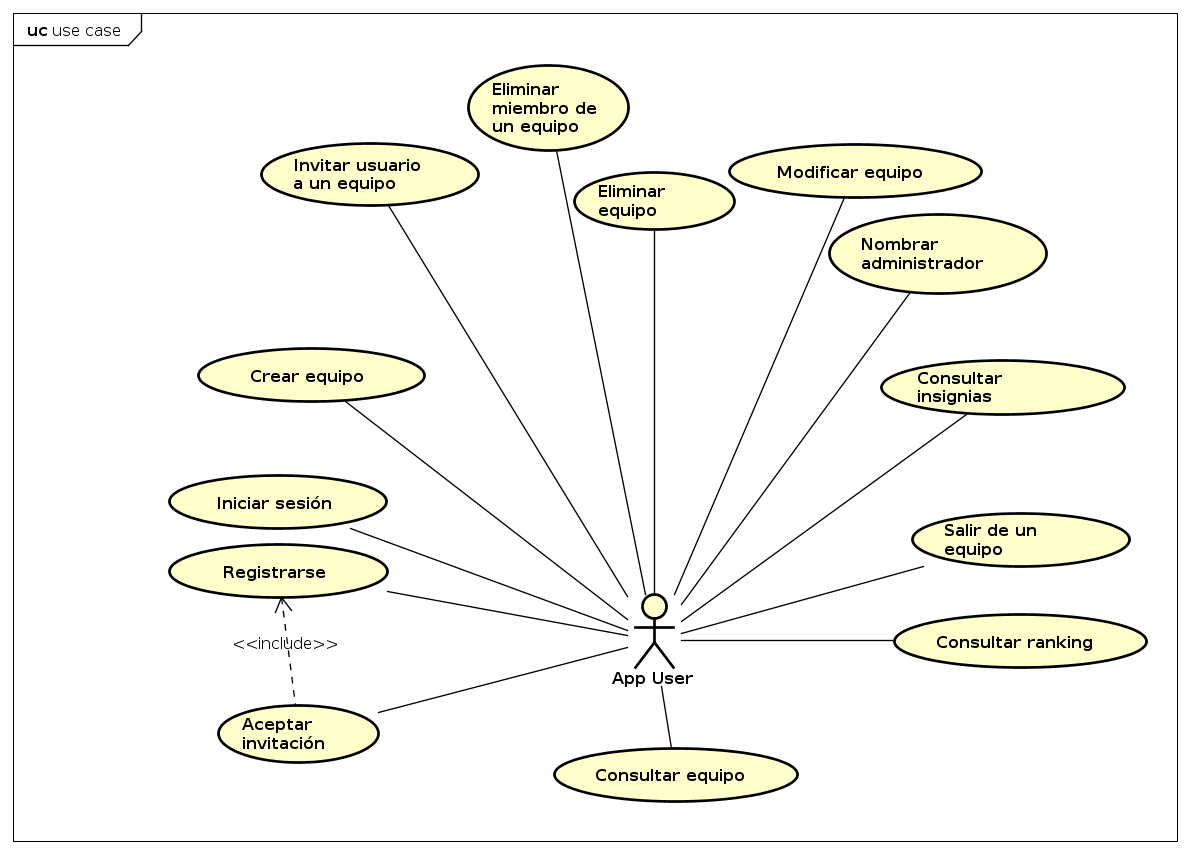
\includegraphics[scale=0.47]{images/usecase0.png}
\caption{Diagrama de casos de uso. Parte I.}
\end{center}
\end{figure}

\begin{figure}[H]
\begin{center}
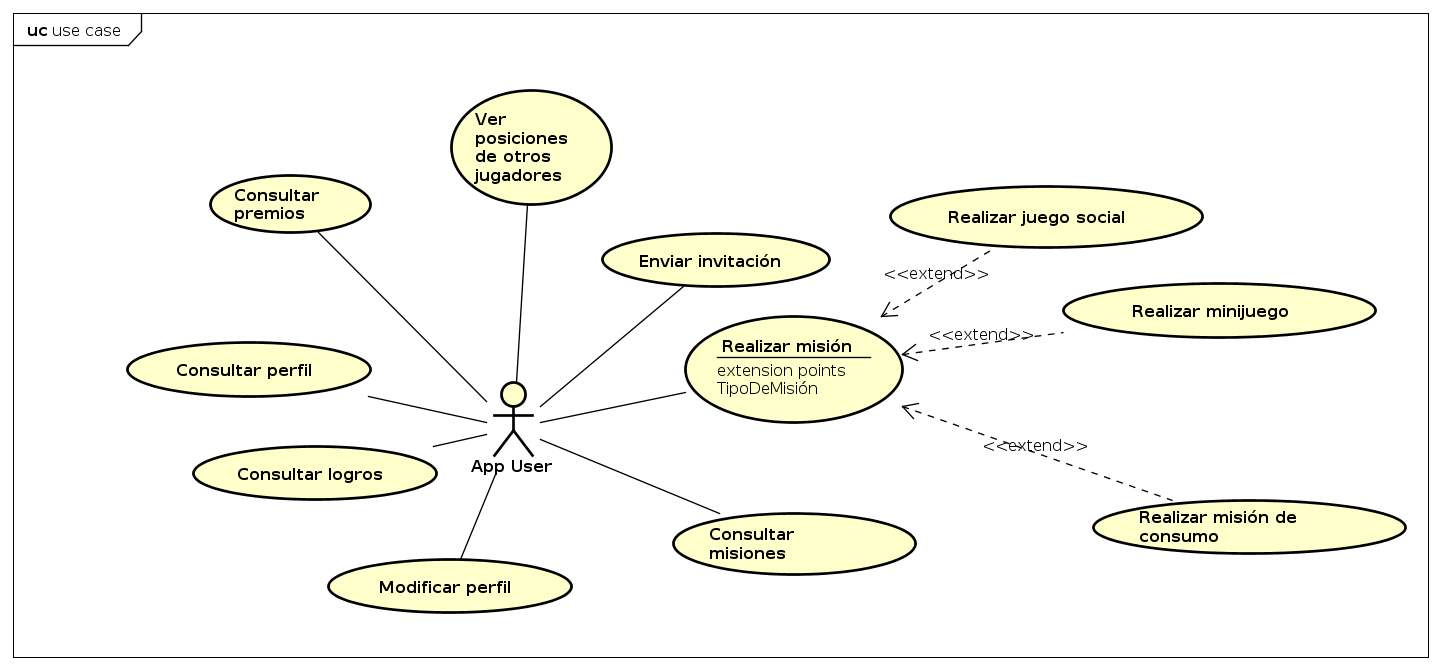
\includegraphics[scale=0.47]{images/usecase1.png}
\caption{Diagrama de casos de uso. Parte II.}
\end{center}
\end{figure}

\subsubsection{Actores}

Se identifican un único actor:

\begin{itemize}
\item \textbf{App user:} Es el actor base de Route66App, en su parte de aplicación móvil. Realiza todas las funciones: crear grupos, gestionar aquellos en los que actúa como administrador, cumplir misiones, realizar consumos, etcétera.
\end{itemize}

\subsubsection{Casos de uso}

\newcounter{usecase}\stepcounter{usecase}


\begin{usecase}
  \addheading{\textbf{CU\arabic{usecase}}}{Modificar equipo} 
  \addrow{Actor}{App user.}
  \addrow{Precondiciones}{El usuario ha iniciado sesión en el sistema.}
  \addrow{Postcondiciones}{Ninguna.}
  \addrow{Flujo principal}{
  		\begin{enumerate}
  		\item El usuario selecciona “Gestionar un equipo“. %1
        \item El sistema muestra al usuario el listado de equipos. %2
        \item El usuario selecciona un equipo de la lista. %3
        \item El sistema muestra el conjunto de parámetros de configuración del grupo, así como el valor de los mismos. %4
        \item El usuario elige un parámetro y lo modifica. %5
        \item El sistema actualiza la configuración del grupo. %6
  		\end{enumerate}
  }
  \addrow{Flujos alternativos}{
  		\begin{itemize}
  		\item 1a 3a 5a El usuario cancela la operación. En este caso, el caso de uso termina y queda sin efecto.
  		\item 2a El sistema no encuentra ningún equipo administrado por el usuario. En ese caso, se muestra un mensaje y el caso de uso queda sin efecto.
  		\item 6a El parámetro introducido por el usuario no es válido (porque se ha introducido en un formato incorrecto). En ese caso, se notifica al usuario y se vuelve al paso 5.
  		\end{itemize}
  }
\end{usecase}\\\stepcounter{usecase}

\begin{usecase}
  \addheading{\textbf{CU\arabic{usecase}}}{Invitar usuario al equipo} 
  \addrow{Actor}{App user}
  \addrow{Precondiciones}{El usuario ha iniciado sesión en el sistema.}
  \addrow{Postcondiciones}{Ninguna.}
  \addrow{Flujo principal}{
  		\begin{enumerate}
  		\item El usuario elige “Invitar usuario al equipo“. %1
  		\item El sistema muestra al usuario el listado de equipos que administra. %2
  		\item El usuario elige un equipo. %3
  		\item El sistema comprueba que el equipo tenga menos de 10 miembros. %4
  		\item El sistema pregunta al usuario el correo electrónico o número de teléfono del usuario que desea agregar. %5
  		\item El usuario introduce la información. %6
  		\item El sistema comprueba el dato y añade al usuario al equipo. %7
  		\end{enumerate}
  }
  \addrow{Flujos alternativos}{
  		\begin{itemize}
  		\item 1a 3a 6a El usuario cancela la operación. En este caso, el caso de uso termina y queda sin efecto.
  		\item 4a El usuario ha elegido un grupo que tiene 10 usuarios o más. En este caso, el sistema muestra un mensaje y vuelve al paso 2.
  		\item 5a El correo electrónico o teléfono del usuario no se corresponde con un usuario de la aplicación. En ese caso se notifica al usuario y se vuelve al paso 5, indicando en el formulario el correo electrónico o teléfono que hubiera introducido el usuario con anterioridad.
  		\end{itemize}
  }
\end{usecase}\\\stepcounter{usecase}

\begin{usecase}
  \addheading{\textbf{CU\arabic{usecase}}}{Nombrar administrador} 
  \addrow{Actor}{App user}
  \addrow{Precondiciones}{El usuario ha iniciado sesión en el sistema.}
  \addrow{Postcondiciones}{Ninguna.}
  \addrow{Flujo principal}{
  		\begin{enumerate}
  		\item El usuario elige “Nombrar administrador“. %1
  		\item El sistema muestra al usuario el listado de equipos que administra. %2
  		\item El usuario elige un equipo. %3
  		\item El sistema muestra al usuario el conjunto de miembros del equipo %4
  		\item El usuario elige un miembro. %5
  		\item El sistema actualiza la configuración de ese equipo. %6
  		\end{enumerate}
  }
  \addrow{Flujos alternativos}{
  		\begin{itemize}
  		\item 1a 3a 5a El usuario cancela la operación. En este caso, el caso de uso termina y queda sin efecto.
  		\end{itemize}
  }
\end{usecase}\\\stepcounter{usecase}

\begin{usecase}
  \addheading{\textbf{CU\arabic{usecase}}}{Eliminar miembro del equipo} 
  \addrow{Actor}{App user}
  \addrow{Precondiciones}{El usuario ha iniciado sesión en el sistema.}
  \addrow{Postcondiciones}{Ninguna.}
  \addrow{Flujo principal}{
  		\begin{enumerate}
  		\item El usuario elige “Eliminar miembro del equipo“. %1
  		\item El sistema muestra al usuario el listado de equipos que administra. %2
  		\item El usuario elige un equipo. %3
  		\item El sistema muestra al usuario el conjunto de miembros del equipo %4
  		\item El usuario elige un miembro. %5
  		\item El sistema actualiza la configuración de ese equipo. %6
  		\end{enumerate}
  }
  \addrow{Flujos alternativos}{
  		\begin{itemize}
  		\item 1a 3a 5a El usuario cancela la operación. En este caso, el caso de uso termina y queda sin efecto.
  		\end{itemize}
  }
\end{usecase}\\\stepcounter{usecase}

\begin{usecase}
  \addheading{\textbf{CU\arabic{usecase}}}{Eliminar equipo} 
  \addrow{Actor}{App user}
  \addrow{Precondiciones}{El usuario ha iniciado sesión en el sistema.}
  \addrow{Postcondiciones}{Ninguna.}
  \addrow{Flujo principal}{
  		\begin{enumerate}
  		\item El usuario elige “Eliminar equipo“. %1
  		\item El sistema muestra al usuario el listado de equipos que administra. %2
  		\item El usuario elige un equipo. %3
  		\item El sistema elimina el equipo %4
  		\end{enumerate}
  }
  \addrow{Flujos alternativos}{
  		\begin{itemize}
  		\item 1a 3a El usuario cancela la operación. En este caso, el caso de uso termina y queda sin efecto.
  		\end{itemize}
  }
\end{usecase}\\\stepcounter{usecase}


\begin{usecase}
  \addheading{\textbf{CU\arabic{usecase}}}{Realizar misión} 
  \addrow{Actor}{App user}
  \addrow{Precondiciones}{El usuario ha iniciado sesión en el sistema.}
  \addrow{Postcondiciones}{Ninguna.}
  \addrow{Flujo principal}{
  		\begin{enumerate}
  		\item El usuario elige “Realizar misión“. %1
  		\item El sistema muestra al usuario el conjunto de niveles con los que cuenta la aplicación. %2
  		\item El usuario escoge un nivel. %3
  		\item El sistema muestra al usuario las misiones de ese nivel. %4.
  		\item El usuario escoge la misión que desea realizar %5.
  		\item El sistema busca en la base de datos si hay registros de anteriores intentos de resolver la misión y muestra al usuario la misión (\textit{punto de extensión TipoDeMisión}). %6
  		\item El usuario completa la misión y genera el logro asociado a la misma.%7
  		\item El sistema actualiza la información, guardando que el usuario ha completado la misión. %8
  		\end{enumerate}
  }
  \addrow{Flujos alternativos}{
  		\begin{itemize}
  		\item 1a 3a 5a 7a El usuario cancela la operación. En este caso, el caso de uso termina y queda sin efecto.
        \item 3b El usuario no selecciona el nivel que le corresponde completar (el nivel más bajo al que le falte por completar misiones). En ese caso, el sistema muestra un mensaje y vuelve al paso 2.
        
        \item 6a El usuario ha escogido una misión (\textit{punto de extensión TipoDeMisión}) de tipo \textit{“juego social“}. En este caso, se acude al caso de uso “Realizar juego social“, pasando a este caso de uso el identificador de la misión que se va a realizar.
        
        \item 6b El usuario ha escogido una misión (\textit{punto de extensión TipoDeMisión}) de tipo \textit{“minijuego“}. En este caso, se acude al caso de uso “Realizar minijuego“, pasando a este caso de uso el identificador de la misión que se va a realizar.
        
        \item 6c El usuario ha escogido una misión (\textit{punto de extensión TipoDeMisión}) de tipo \textit{“consumo“}. En este caso, se acude al caso de uso “Realizar misión de consumo“, pasando a este caso de uso el identificador de la misión que se va a realizar.
        
        \item 7b El usuario no completa la misión. En ese caso, se pregunta al usuario si desea volver a intentar
  		\end{itemize}
  }
\end{usecase}\\\stepcounter{usecase}

\begin{usecase}
  \addheading{\textbf{CU\arabic{usecase}}}{Realizar misión de consumo mínimo} 
  \addrow{Actor}{App user}
  \addrow{Precondiciones}{El usuario ha iniciado sesión en el sistema.}
  \addrow{Postcondiciones}{Ninguna.}
  \addrow{Flujo principal}{
  		\begin{enumerate}
  		\item El sistema obtiene los detalles de la misión, a partir del identificador de misión que se ha proporcionado.
  		\item El sistema muestra al usuario el consumo que debe realizar para marcar la misión como completada.
  		\item El sistema comprueba si existe algún registro de consumo asociado al usuario que tenga un importe, como mínimo, el que exige la misión para ser completada. Este registro deberá haberse registrado con fecha posterior a la hora de entrada, por primera vez a la actividad.
  		\end{enumerate}
  }
  \addrow{Flujos alternativos}{
  		\begin{itemize}
  		\item 3a No existe ningún registro de consumo que cumpla tales caracterísiticas, en ese caso, se informa al usuario.
  		\end{itemize}
  }
\end{usecase}\\\stepcounter{usecase}

\begin{usecase}
  \addheading{\textbf{CU\arabic{usecase}}}{Realizar minijuego.} 
  \addrow{Actor}{App user}
  \addrow{Precondiciones}{El usuario ha iniciado sesión en el sistema.}
  \addrow{Postcondiciones}{Ninguna.}
  \addrow{Flujo principal}{
  		\begin{enumerate}
  		\item El sistema obtiene los detalles de la misión, a partir del identificador de misión que se ha proporcionado. %1
  		\item El sistema muestra al usuario el minijuego asociado a la misión. %2
  		\item El sistema introduce un escuchador detrás del navegador donde se muestra el juego para obtener los resultados del mismo. %3
  		\item El sistema da el control del mismo al juego. %4
  		\item El sistema recibe los resultados del juego por medio del escuchador. %5
  		\item El sistema comprueba que los resultados del juego estén dentro del intervalo de lo pedido para la misión. %6
  		\end{enumerate}
  }
  \addrow{Flujos alternativos}{
  		\begin{itemize}
  		\item 6a Los parámetros recibidos no se corresponden con los valores que se exigen para completar la misión. En ese caso, se muestra un mensaje al usuario, se envía un mensaje de reporte al servidor y se pregunta al usuario si desea volver a intentar la misión. En caso afirmativo se volvería al paso 2. En caso negativo, se saldría de los casos de uso Realizar misión y Realizar minijuego.
  		\end{itemize}
  }
\end{usecase}\\\stepcounter{usecase}

\begin{usecase}
  \addheading{\textbf{CU\arabic{usecase}}}{Realizar juego social.} 
  \addrow{Actor}{App user}
  \addrow{Precondiciones}{El usuario ha iniciado sesión en el sistema.}
  \addrow{Postcondiciones}{Ninguna.}
  \addrow{Flujo principal}{
  		\begin{enumerate}
  		\item El sistema obtiene los detalles de la misión, a partir del identificador de misión que se ha proporcionado.
  		\item El sistema muestra al usuario el reto social que debe realizar para marcar la misión como completada.
  		\item El sistema comprueba si existe algún registro de reto socal asociado al usuario. Este registro deberá haberse registrado con fecha posterior a la hora de entrada, por primera vez a la actividad.
  		\end{enumerate}
  }
  \addrow{Flujos alternativos}{
  		\begin{itemize}
  		\item 3a No existe ningún registro de consumo que cumpla tales caracterísiticas, en ese caso, se informa al usuario.
  		\end{itemize}
  }
\end{usecase}\\\stepcounter{usecase}

\begin{usecase}
  \addheading{\textbf{CU\arabic{usecase}}}{Consultar misiones} 
  \addrow{Actor}{App user}
  \addrow{Precondiciones}{El usuario ha iniciado sesión en el sistema.}
  \addrow{Postcondiciones}{Ninguna.}
  \addrow{Flujo principal}{
  		\begin{enumerate}
  		\item El usuario elige “Consultar misiones“. %1
  		\item El sistema muestra al usuario el listado de niveles, destacando aquellos niveles que ya haya completado y marcando de una forma especial aquel nivel en el que se encuentre el usuario (que tenga misiones sin completar). %2
  		\item El usuario selecciona un nivel. %3
  		\item El sistema muestra al usuario las distintas misiones que conforman el nivel, destacando aquellas que hayan sido resueltas con anterioridad. %4
  		\end{enumerate}
  }
  \addrow{Flujos alternativos}{
  		\begin{itemize}
  		\item 3a. El usuario cancela la operación. En este caso, el caso de uso termina y queda sin efecto.
  		\item 3b. El usuario ha seleccionado un nivel superior a aquel en el que se encuentra el usuario. En este caso, se muestra un mensaje al usuario y se vuelve al paso 2.
  		\end{itemize}
  }
\end{usecase}\\\stepcounter{usecase}

\begin{usecase}
  \addheading{\textbf{CU\arabic{usecase}}}{Modificar perfil} 
  \addrow{Actor}{App user}
  \addrow{Precondiciones}{El usuario ha iniciado sesión en el sistema.}
  \addrow{Postcondiciones}{Ninguna.}
  \addrow{Flujo principal}{
  		\begin{enumerate}
  		\item El usuario elige “Modificar perfil“. %1
  		\item El sistema muestra al usuario el conjunto de parámetros que puede modificar y los valores que tiene asociados. %2
  		\item El usuario elige un parámetro y lo modifica. %3
  		\item El sistema actualiza el nuevo valor. %4
  		\end{enumerate}
  }
  \addrow{Flujos alternativos}{
  		\begin{itemize}
  		\item 1a 3a El usuario cancela la operación. En este caso, el caso de uso termina y queda sin efecto.
  		\item 4a El parámetro introducido por el usuario no es válido (porque se ha introducido en un formato incorrecto). En ese caso, se notifica al usuario y se vuelve al paso 5.
  		\end{itemize}
  		}
\end{usecase}\\\stepcounter{usecase}

\begin{usecase}
  \addheading{\textbf{CU\arabic{usecase}}}{Consultar perfil} 
  \addrow{Actor}{App user}
  \addrow{Precondiciones}{El usuario ha iniciado sesión en el sistema.}
  \addrow{Postcondiciones}{Ninguna.}
  \addrow{Flujo principal}{
  		\begin{enumerate}
  		\item El usuario elige “Consultar perfil“.
  		\item El sistema muestra al usuario su perfil, incluidos aquellos detalles como sus  “porcentajes de compromiso“ con la aplicación. (Ver página \pageref{rfcompromiso}).
  		\end{enumerate}
  }
\end{usecase}\\\stepcounter{usecase}

\begin{usecase}
  \addheading{\textbf{CU\arabic{usecase}}}{Consultar logros} 
  \addrow{Actor}{App user}
  \addrow{Precondiciones}{El usuario ha iniciado sesión en el sistema.}
  \addrow{Postcondiciones}{Ninguna.}
  \addrow{Flujo principal}{
  		\begin{enumerate}
  		\item El usuario elige “Consultar mis logros“.
  		\item El sistema muestra al usuario los logros realizados, ordenados por fecha.
  		\end{enumerate}
  }
\end{usecase}\\\stepcounter{usecase}

\begin{usecase}
  \addheading{\textbf{CU\arabic{usecase}}}{Consultar insignias} 
  \addrow{Actor}{App user}
  \addrow{Precondiciones}{El usuario ha iniciado sesión en el sistema.}
  \addrow{Postcondiciones}{Ninguna.}
  \addrow{Flujo principal}{
  		\begin{enumerate}
  		\item El usuario elige “Consultar mis insignias“.
  		\item El sistema muestra al usuario las insignias obtenidas, ordenadas por fecha.
  		\end{enumerate}
  }
\end{usecase}\\\stepcounter{usecase}

\begin{usecase}
  \addheading{\textbf{CU\arabic{usecase}}}{Consultar código QR} 
  \addrow{Actor}{App user}
  \addrow{Precondiciones}{El usuario ha iniciado sesión en el sistema.}
  \addrow{Postcondiciones}{Ninguna.}
  \addrow{Flujo principal}{
  		\begin{enumerate}
  		\item El usuario elige “Consultar código QR“.
  		\item El sistema muestra al usuario su código QR.
  		\end{enumerate}
  }
\end{usecase}\\\stepcounter{usecase}

\begin{usecase}
  \addheading{\textbf{CU\arabic{usecase}}}{Consultar ranking} 
  \addrow{Actor}{App user}
  \addrow{Precondiciones}{El usuario ha iniciado sesión en el sistema.}
  \addrow{Postcondiciones}{Ninguna.}
  \addrow{Flujo principal}{
  		\begin{enumerate}
  		\item El usuario elige “Consultar ranking“.
  		\item El sistema muestra al usuario el ranking global de usuarios, ordenados por los puntos obtenidos.
  		\end{enumerate}
  }
\end{usecase}\\\stepcounter{usecase}

\begin{usecase}
  \addheading{\textbf{CU\arabic{usecase}}}{Consultar equipo} 
  \addrow{Actor}{App user}
  \addrow{Precondiciones}{El usuario ha iniciado sesión en el sistema.}
  \addrow{Postcondiciones}{Ninguna.}
  \addrow{Flujo principal}{
  		\begin{enumerate}
  		\item El usuario elige “Consultar equipo“. %1
  		\item El sistema muestra al usuario el listado de equipos en los que es miembro. %2
  		\item El usuario selecciona un equipo. %3
  		\item El sistema muestra al usuario los detalles de ese equipo (miembros, nombre, visibilidad y avatar). %4
  		\end{enumerate}
  }
  \addrow{Flujos alternativos}{
  		\begin{itemize}
  		\item 1a 3a El usuario cancela la operación. En este caso, el caso de uso termina y queda sin efecto.
  		\item 2a El sistema no encuentra ningún equipo en el que se encuentre el miembro. En ese caso, se muestra un mensaje al usuario y el caso de uso queda sin efecto.
  		\end{itemize}
  }
\end{usecase}\\\stepcounter{usecase}

\begin{usecase}
  \addheading{\textbf{CU\arabic{usecase}}}{Crear equipo} 
  \addrow{Actor}{App user}
  \addrow{Precondiciones}{El usuario ha iniciado sesión en el sistema.}
  \addrow{Postcondiciones}{Ninguna.}
  \addrow{Flujo principal}{
  		\begin{enumerate}
  		\item El usuario elige “Crear equipo“. %1
  		\item El sistema pregunta al usuario el nombre del equipo, así como el tipo de visibilidad del equipo. %2
  		\item El usuario introduce los datos. %3
  		\item El sistema comprueba los datos y crea el equipo. %4
  		\item Se pasa al caso de uso “Invitar usuario al equipo“, indicando cuál es el equipo que acaba de ser recién creado.
  		\end{enumerate}
  }
  \addrow{Flujos alternativos}{
  		\begin{itemize}
  		\item 1a 3a 5a El usuario cancela la operación. En este caso, el caso de uso termina y queda sin efecto.
  		\item 4a El usuario ha introducido un nombre de equipo ya existente. En este caso, el sistema muestra un mensaje y le vuelve a solicitar el dato.
  		\end{itemize}
  }
\end{usecase}\\\stepcounter{usecase}

\begin{usecase}
  \addheading{\textbf{CU\arabic{usecase}}}{Registrarse} 
  \addrow{Actor}{App user}
  \addrow{Precondiciones}{Ninguna.}
  \addrow{Postcondiciones}{Ninguna.}
  \addrow{Flujo principal}{
  		\begin{enumerate}
  		\item El usuario elige “Registrarse“. %1
  		\item El sistema pregunta al usuario cuál es su correo electrónico, una contraseña, así como su nombre y apellidos. %2
  		\item El usuario introduce la información. %3
  		\item El sistema comprueba la información y crea el usuario. %4
  		\end{enumerate}
  }
  \addrow{Flujos alternativos}{
  		\begin{itemize}
  		\item 1a 3a El usuario cancela la operación. En este caso, el caso de uso termina y queda sin efecto.
  		\item 4a El sistema identifica un usuario ya registrado con el correo electrónico proporcionado. En ese caso, se muestra al usuario un mensaje alertándole y se vuelve al paso 2, pero completando el formulario con la información que ya hubiera introducido el usuario.
  		\end{itemize}
  }
\end{usecase}\\\stepcounter{usecase}

\begin{usecase}
  \addheading{\textbf{CU\arabic{usecase}}}{Aceptar invitación.} 
  \addrow{Actor}{App user}
  \addrow{Precondiciones}{Ninguna.}
  \addrow{Postcondiciones}{Ninguna.}
  \addrow{Nota}{Este caso de uso depende del componente Firebase Invitations, que a su vez depende de Firebase Dynamic Links.}
  \addrow{Flujo principal}{
  		\begin{enumerate}
  		\item El sistema recibe una llamada de Firebase Invitations que le proporciona el identificador de la invitación.
  		\item El sistema busca en la base de datos qué usuario ha enviado esa invitación.
  		\item Se pasa al caso de uso “Registrarse“, junto con el dato del usuario que ha enviado la invitación.
  		\end{enumerate}
  }
  \addrow{Flujos alternativos}{
  		\begin{itemize}
  		\item 1a 2a El usuario cancela la operación. En este caso, el caso de uso termina y queda sin efecto.
  		\end{itemize}
  }
\end{usecase}\\\stepcounter{usecase}

\begin{usecase}
  \addheading{\textbf{CU\arabic{usecase}}}{Enviar invitación} 
  \addrow{Actor}{App user}
  \addrow{Precondiciones}{El usuario ha iniciado sesión en el sistema.}
  \addrow{Postcondiciones}{Ninguna.}
  \addrow{Flujo principal}{
  		\begin{enumerate}
  		\item El usuario elige “Enviar invitación“.
  		\item El sistema genera un identificador único de invitación.
  		\item El sistema muestra al usuario el cuadro de diálogo del sistema para enviar la invitación.
  		\item El usuario comparte la invitación.
  		\end{enumerate}
  }
  \addrow{Flujos alternativos}{
  		\begin{itemize}
  		\item 1a 2a 3a 4a El usuario cancela la operación. En este caso, el caso de uso termina y queda sin efecto.
  		\end{itemize}
  }
\end{usecase}\\\stepcounter{usecase}

\begin{usecase}
  \addheading{\textbf{CU\arabic{usecase}}}{Iniciar sesión} 
  \addrow{Actor}{App user}
  \addrow{Precondiciones}{El usuario ha iniciado sesión en el sistema.}
  \addrow{Postcondiciones}{Ninguna.}
  \addrow{Flujo principal}{
  		\begin{enumerate}
  		\item El usuario elige “Iniciar sesión“. %1
  		\item El sistema pregunta al usuario el correo electrónico, así como su contraseña. %2
  		\item El usuario introduce la información solicitada. %3
  		\item El sistema identifica al usuario. %4
  		\end{enumerate}
  }
  \addrow{Flujos alternativos}{
  		\begin{itemize}
  		\item 1a 3a El usuario cancela la operación. En este caso, el caso de uso termina y queda sin efecto.
  		\item 4a El usuario ha introducido un correo electrónico de un usuario no perteneciente al sistema. En este caso, se notifica al usuario y se vuelve al paso 2.
  		\item 4b El usuario ha introducido una contraseña distinta a la que tiene el usuario. En este caso, se notifica al usuario y se vuelve al paso 2.
  		\end{itemize}
  }
\end{usecase}\\\stepcounter{usecase}

\begin{usecase}
  \addheading{\textbf{CU\arabic{usecase}}}{Ver posiciones de otros jugadores} 
  \addrow{Actor}{App user}
  \addrow{Precondiciones}{El usuario ha iniciado sesión en el sistema.}
  \addrow{Postcondiciones}{Ninguna.}
  \addrow{Flujo principal}{
  		\begin{enumerate}
  		\item El usuario elige un nivel.
  		\item El sistema muestra al usuario las distintas posiciones de los miembros de los equipos a los que pertenece y que se encuentren en ese nivel.
  		\end{enumerate}
  }
  \addrow{Flujos alternativos}{
  		\begin{itemize}
  		\item 2a El usuario no pertenece a ningún equipo o estos solo están integrados por un solo miembro. En este caso,  se muestra un mensaje indicándoselo.
  		\item 2b En el nivel no se encuentra ningún usuario de equipos a los que pertenece el usuario. En este caso, se muestra un mensaje indicándoselo.
  		\end{itemize}
  }
\end{usecase}\\\stepcounter{usecase}

\begin{usecase}
  \addheading{\textbf{CU\arabic{usecase}}}{Consultar premios} 
  \addrow{Actor}{App user}
  \addrow{Precondiciones}{El usuario ha iniciado sesión en el sistema.}
  \addrow{Postcondiciones}{Ninguna.}
  \addrow{Flujo principal}{
  		\begin{enumerate}
  		\item El usuario elige “Consultar mis premios“.
  		\item El sistema muestra al usuario los premios obtenidos que sigan estando vigentes.
  		\end{enumerate}
  }
\end{usecase}\\\stepcounter{usecase}

\subsection{Modelo de dominio}

\begin{figure}[H]
\begin{center}
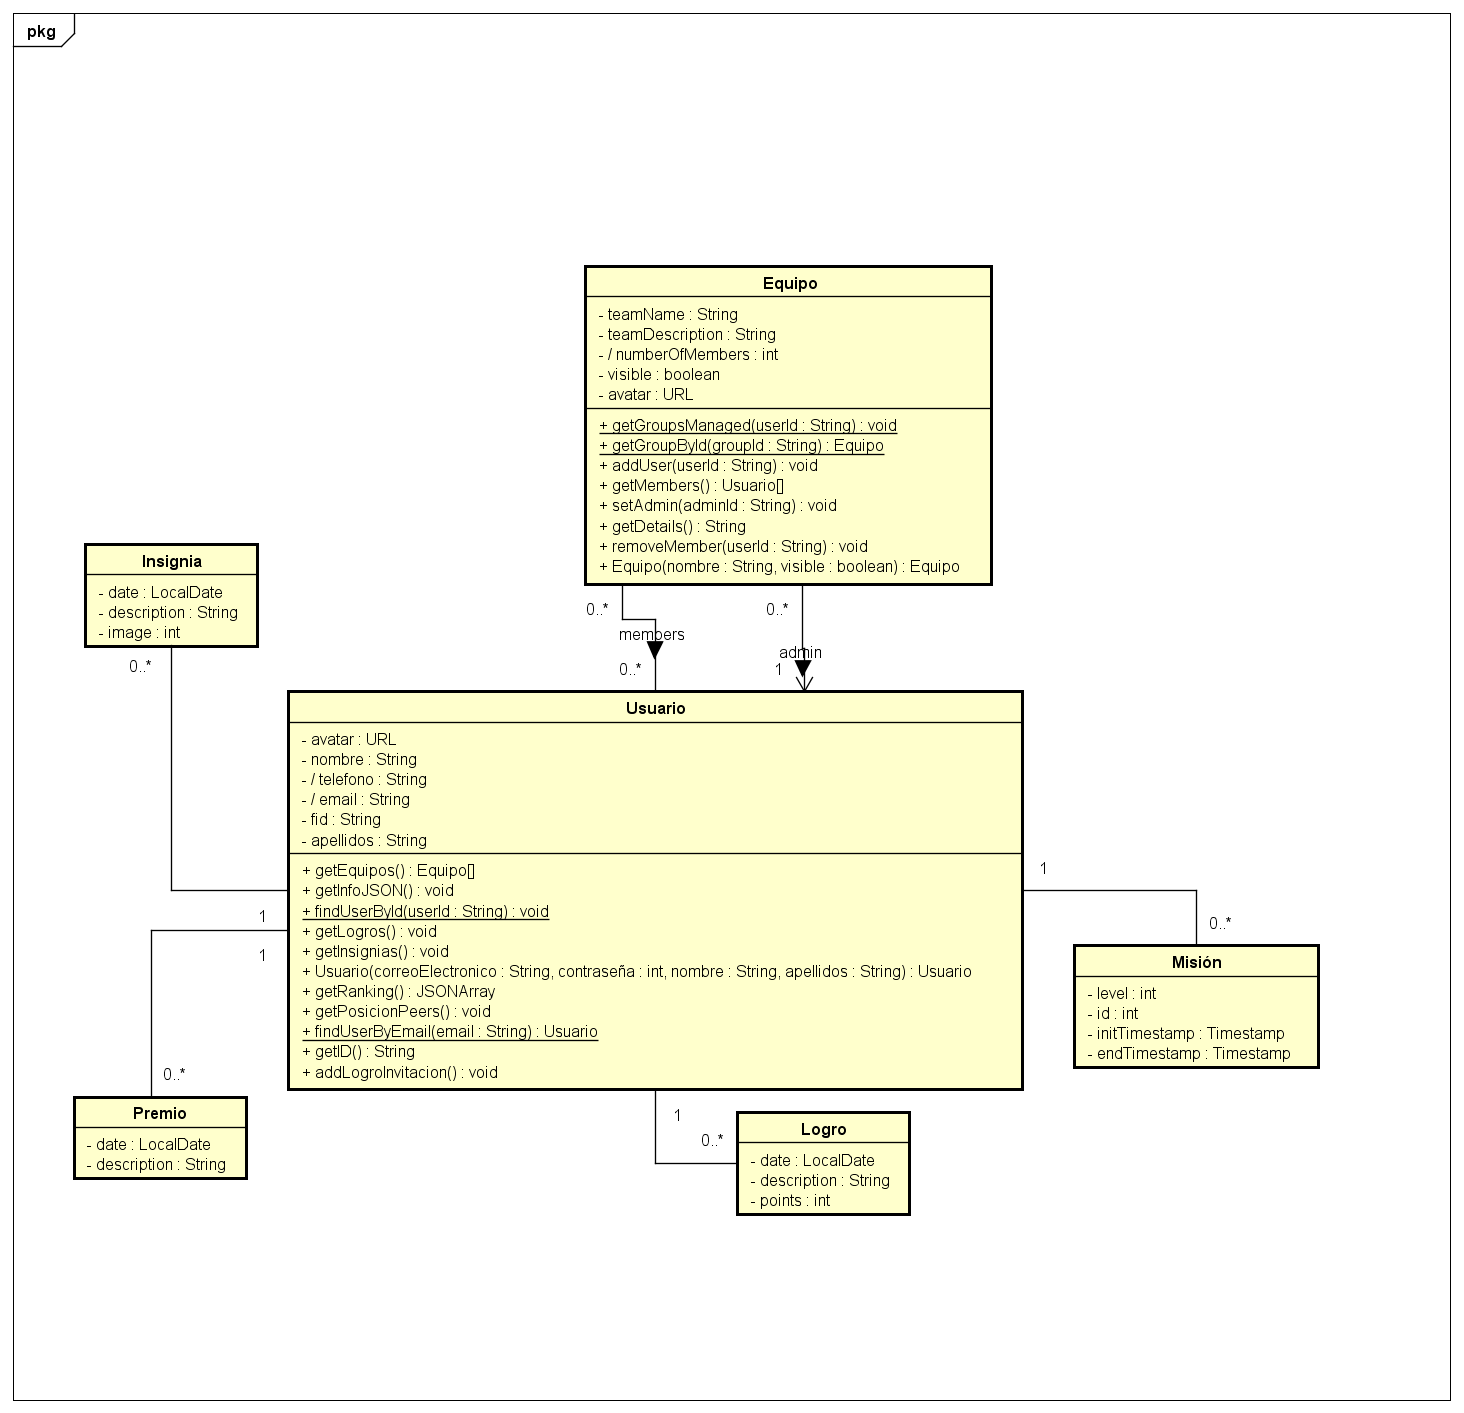
\includegraphics[scale=0.4]{images/clases.png}
\caption{Modelo de dominio}
\end{center}
\end{figure}

\subsection{Diagramas de secuencia}

%0
\begin{figure}[H]
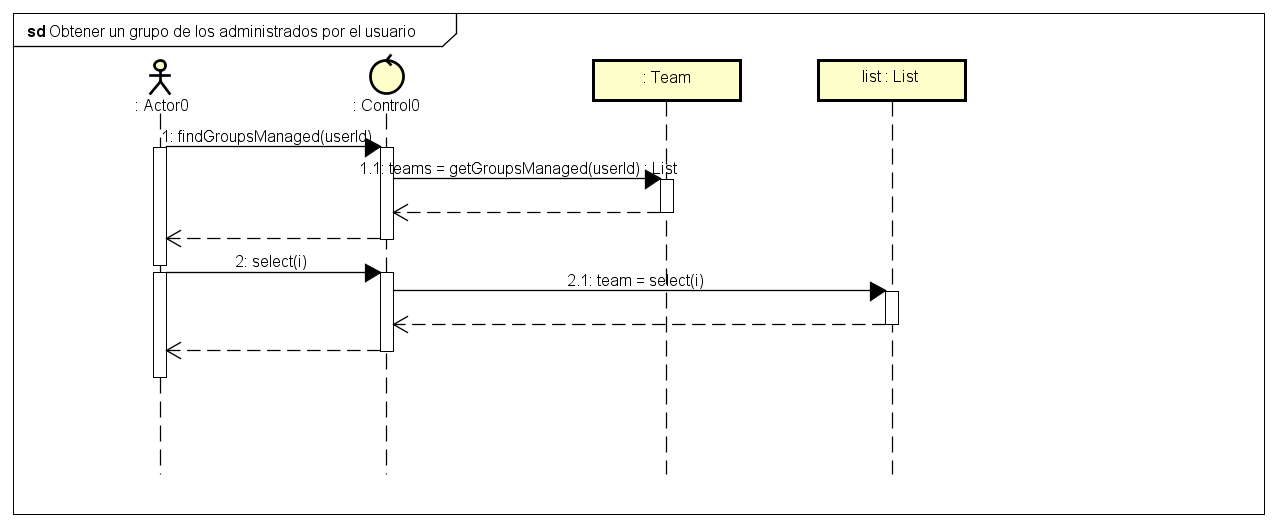
\includegraphics[scale=0.5]{images/sequence/GetAGroupManagedByUser.png}
\caption{Diagrama de secuencia “Obtener un grupo de los administrados por el usuario“}
\end{figure}

%1
\begin{figure}[H]
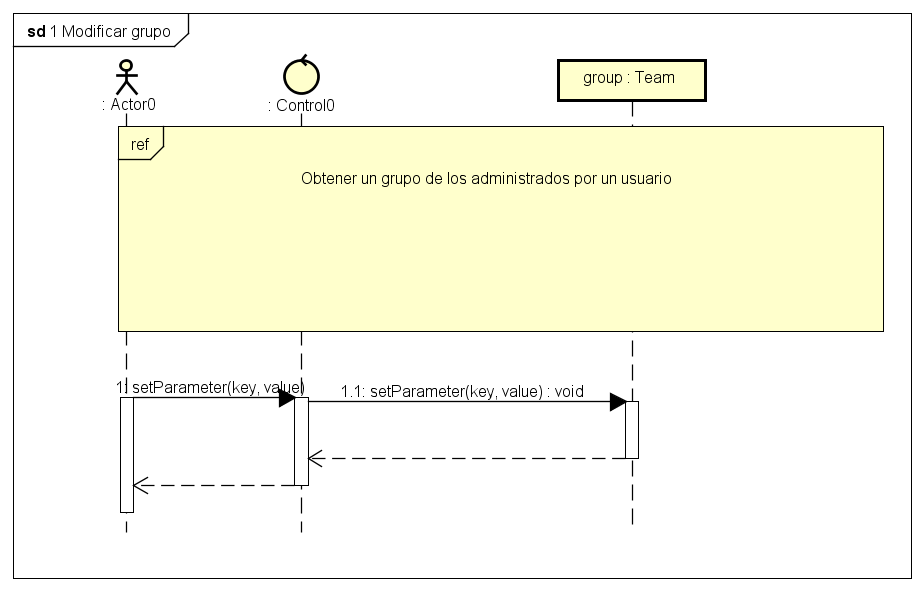
\includegraphics[scale=0.5]{images/sequence/ModifyGroup}
\caption{Diagrama de secuencia del caso de uso “Modificar grupo“}
\end{figure}

%2
\begin{figure}[H]
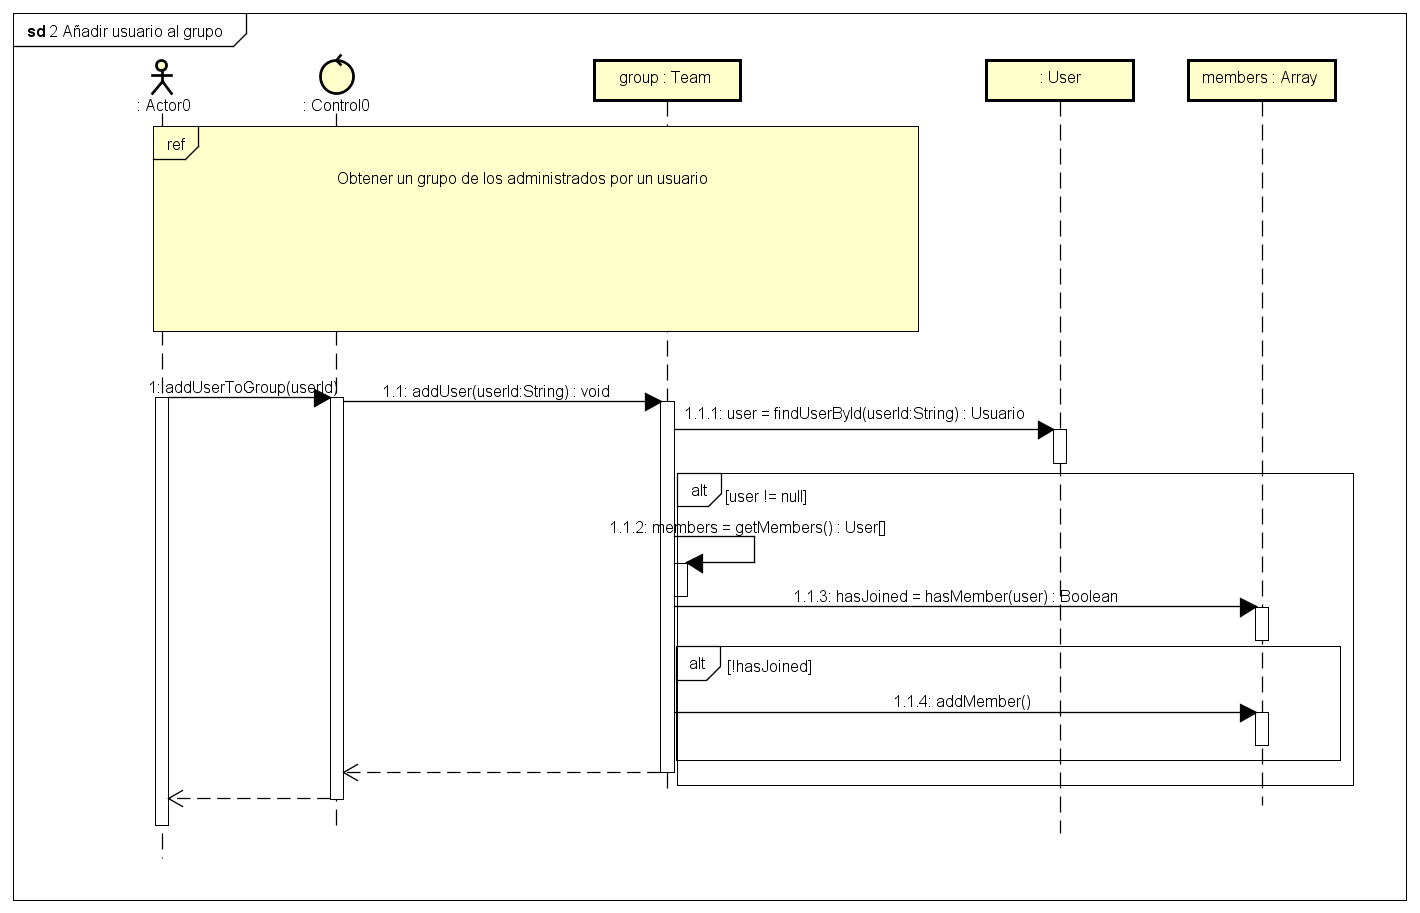
\includegraphics[scale=0.5]{images/sequence/AddUserToGroup}
\caption{Diagrama de secuencia del caso de uso “A\~{n}adir usuario al grupo“}
\end{figure}

%3
\begin{figure}[H]
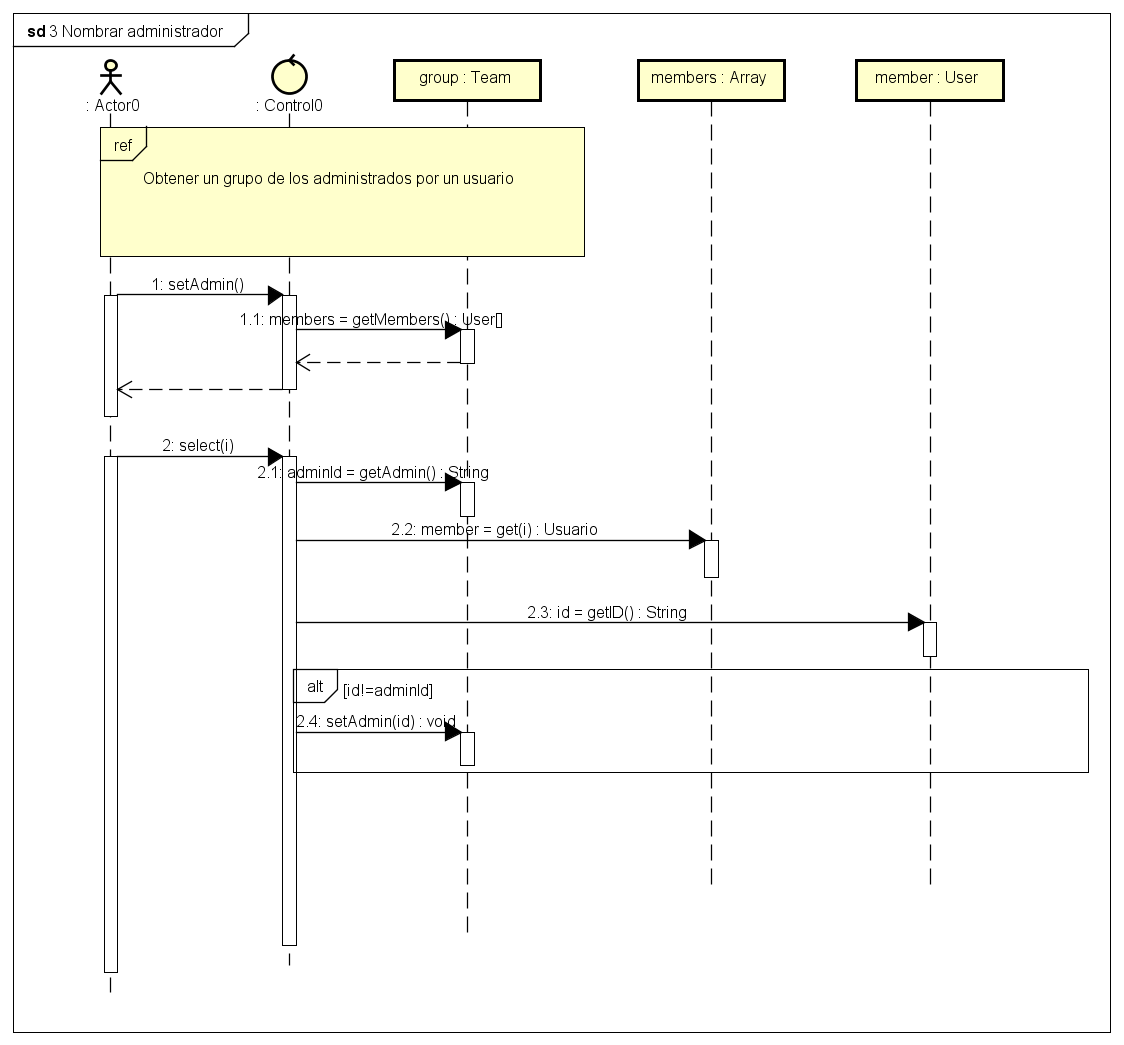
\includegraphics[scale=0.5]{images/sequence/setAdmin}
\caption{Diagrama de secuencia del caso de uso “Nombrar un administrador“}
\end{figure}

%4
\begin{figure}[H]
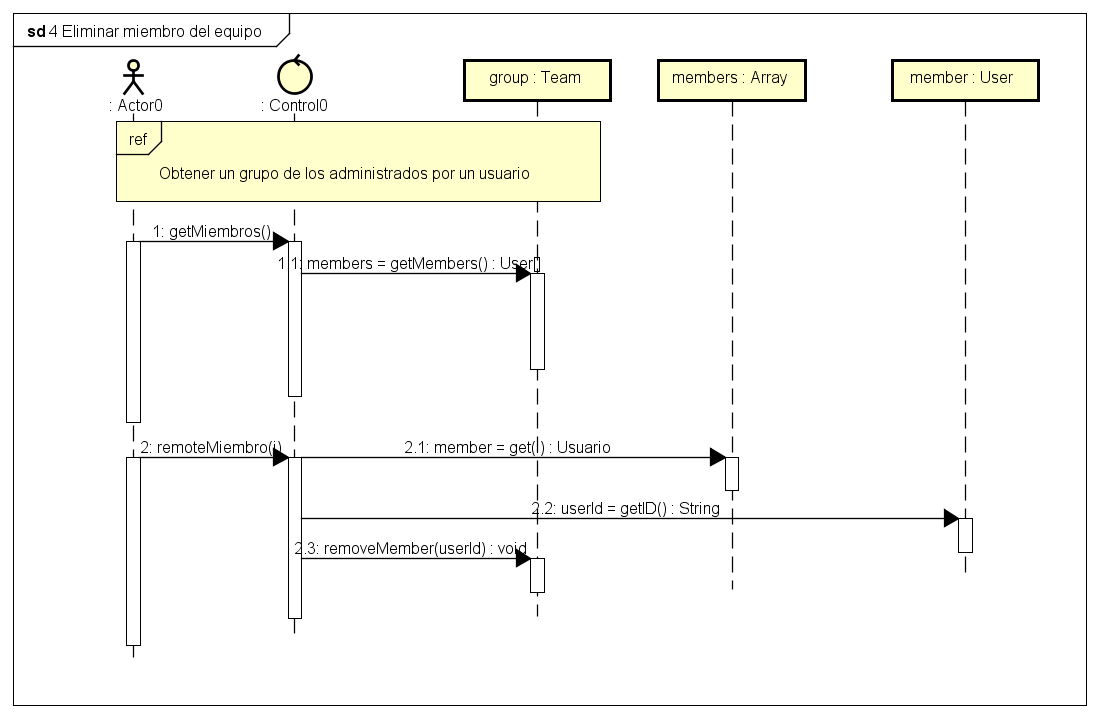
\includegraphics[scale=0.5]{images/sequence/deleleMemberGroup}
\caption{Diagrama de secuencia del caso de uso “Eliminar a un miembro de un equipo“}
\end{figure}

%5
\begin{figure}[H]
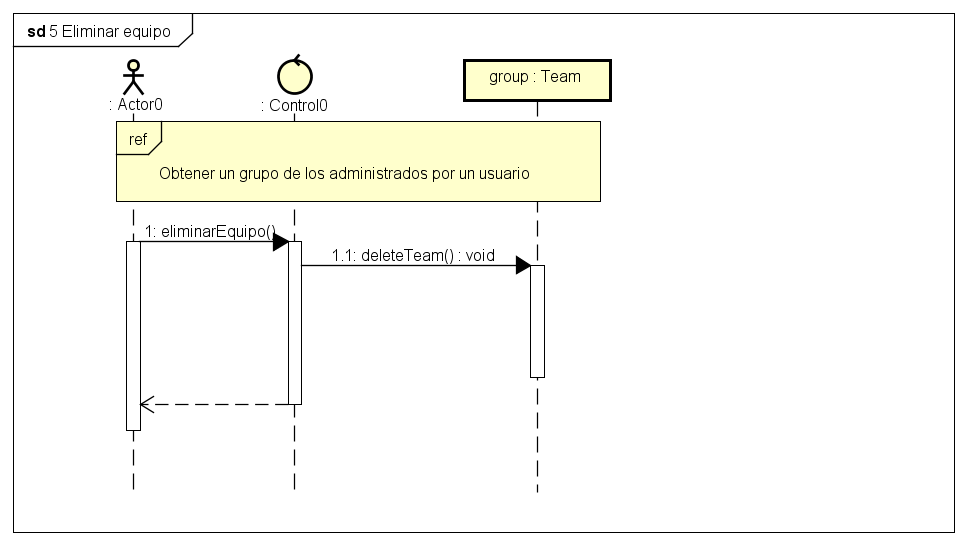
\includegraphics[scale=0.5]{images/sequence/removeTeam}
\caption{Diagrama de secuencia del caso de uso “Eliminar un equipo“}
\end{figure}

%5
\begin{figure}[H]
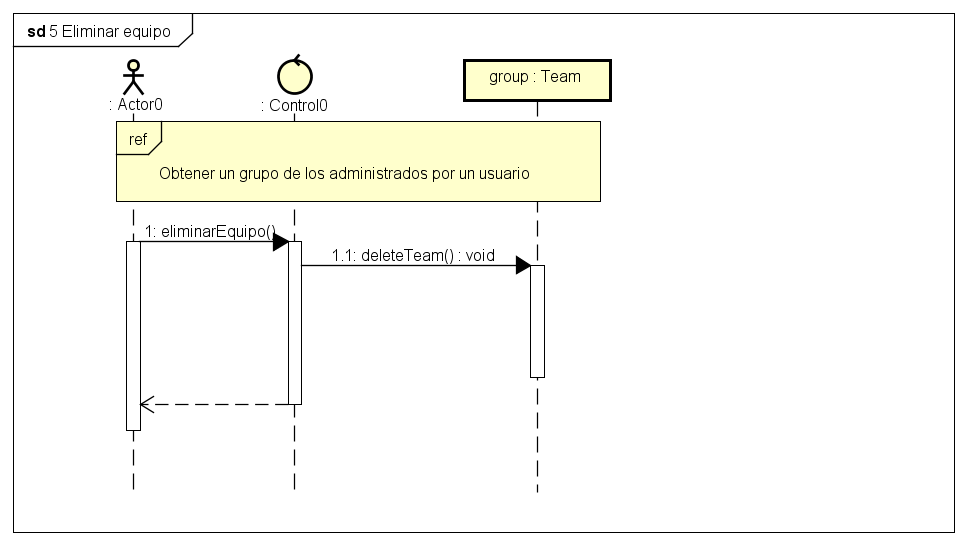
\includegraphics[scale=0.5]{images/sequence/removeTeam}
\caption{Diagrama de secuencia del caso de uso “Eliminar un equipo“}
\end{figure}

%6
\begin{figure}[H]
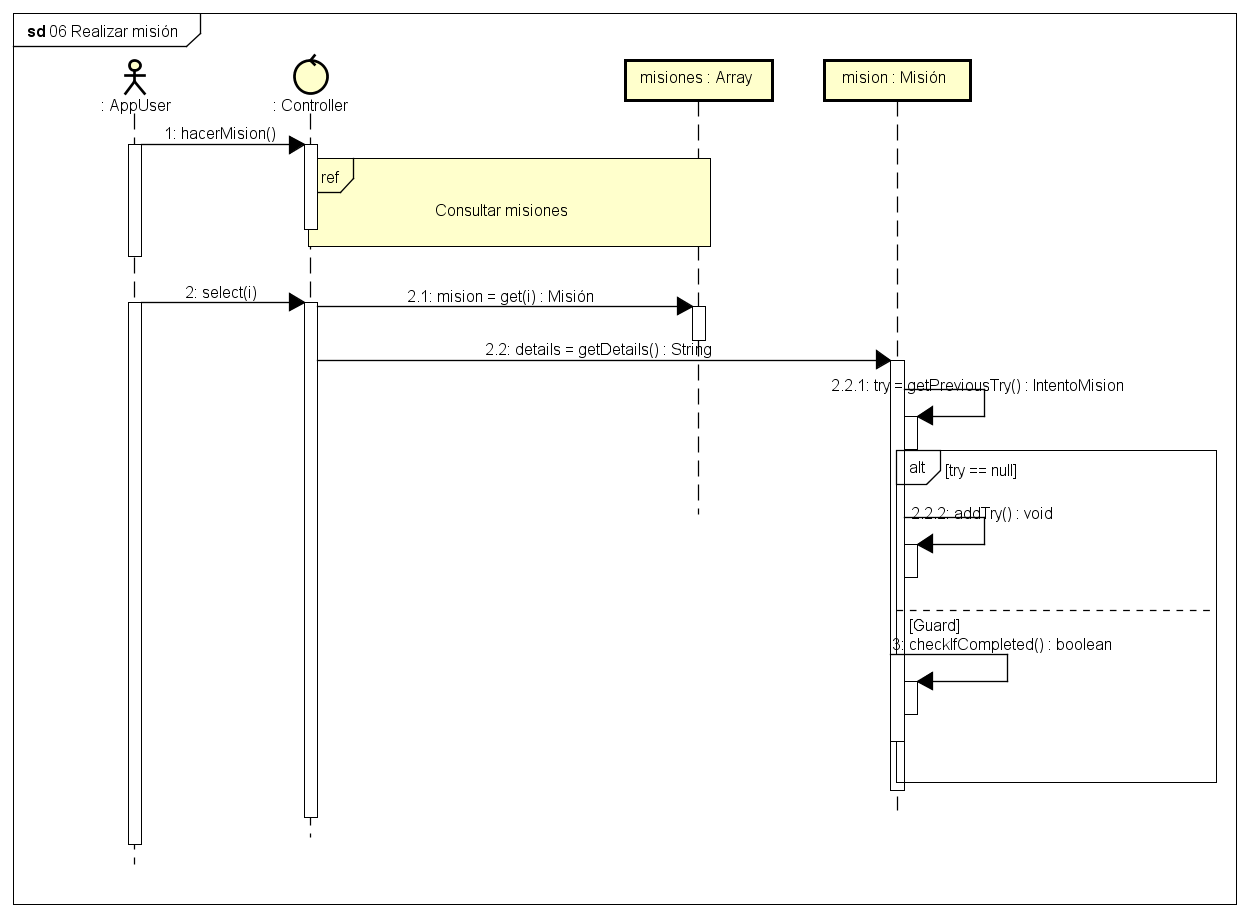
\includegraphics[scale=0.5]{images/sequence/realizarMision}
\caption{Diagrama de secuencia del caso de uso “Realizar misión“}
\end{figure}

%10
\begin{figure}[H]
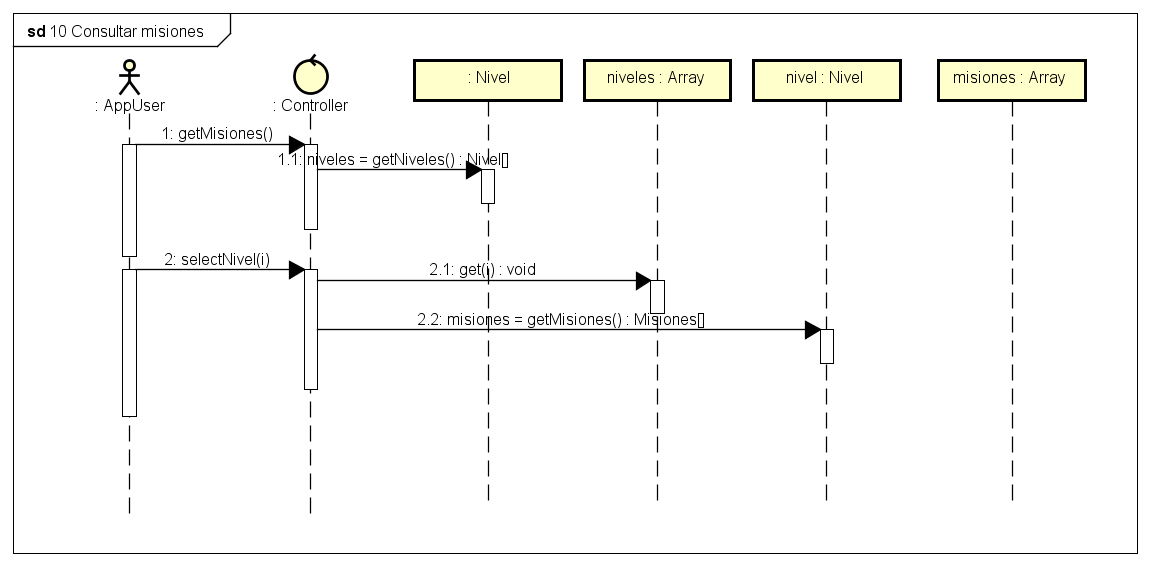
\includegraphics[scale=0.5]{images/sequence/checkMissions}
\caption{Diagrama de secuencia del caso de uso “Consultar misiones“}
\end{figure}

%11
\begin{figure}[H]
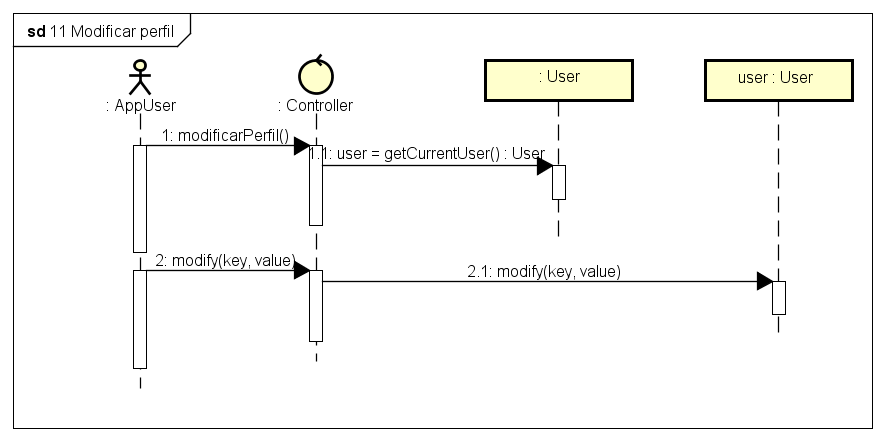
\includegraphics[scale=0.5]{images/sequence/modifyProfile}
\caption{Diagrama de secuencia del caso de uso “Modificar perfil“}
\end{figure}

%12
\begin{figure}[H]
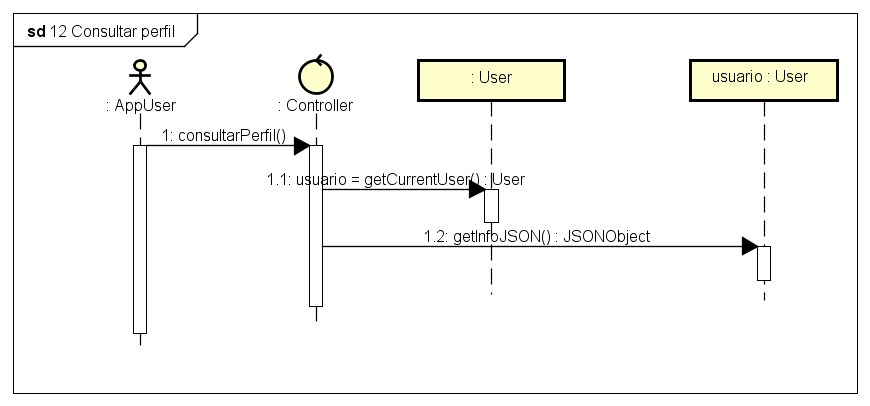
\includegraphics[scale=0.5]{images/sequence/checkProfile}
\caption{Diagrama de secuencia del caso de uso “Consultar perfil“}
\end{figure}

%13
\begin{figure}[H]
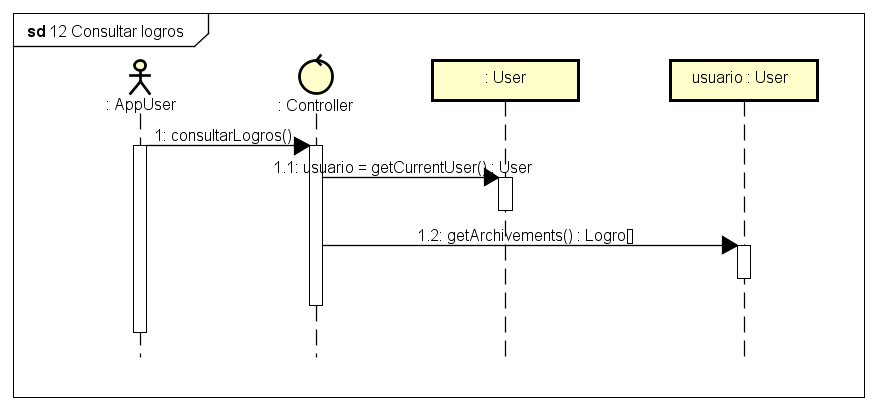
\includegraphics[scale=0.5]{images/sequence/checkArchivements}
\caption{Diagrama de secuencia del caso de uso “Consultar logros“}
\end{figure}

%14
\begin{figure}[H]
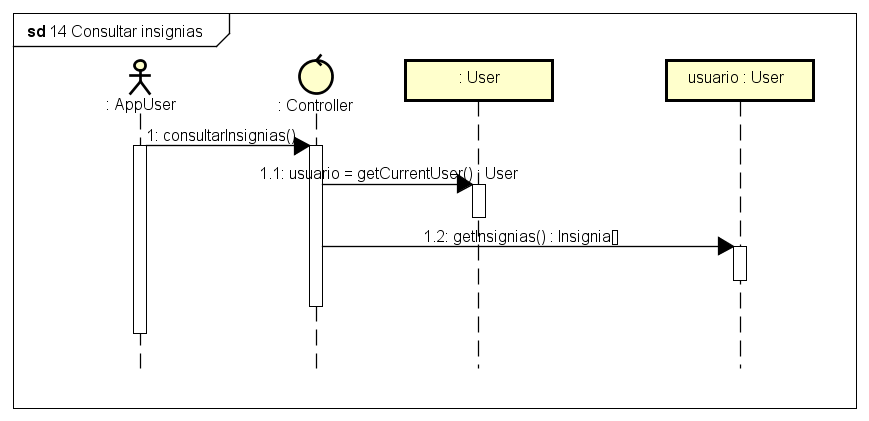
\includegraphics[scale=0.5]{images/sequence/checkInsignias}
\caption{Diagrama de secuencia del caso de uso “Consultar insignias“}
\end{figure}

%15
\begin{figure}[H]
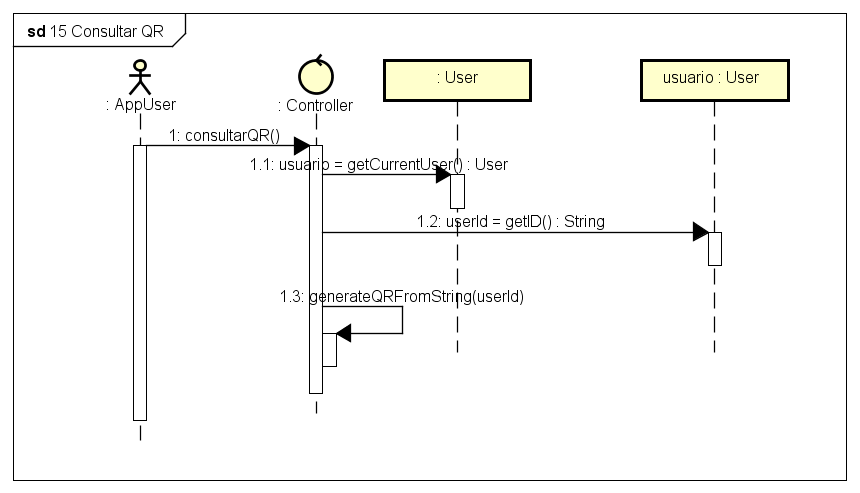
\includegraphics[scale=0.5]{images/sequence/checkQR}
\caption{Diagrama de secuencia del caso de uso “Consultar Código QR“}
\end{figure}

%16
\begin{figure}[H]
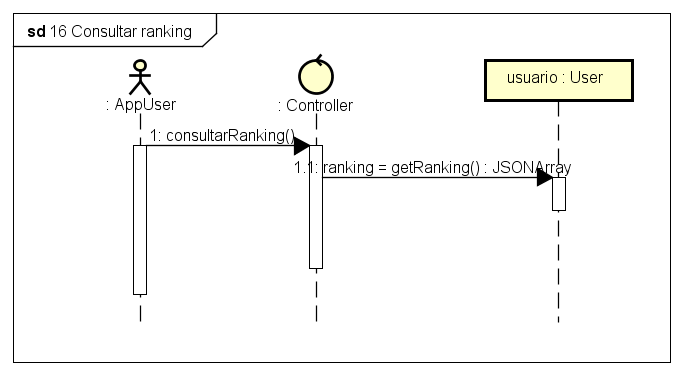
\includegraphics[scale=0.5]{images/sequence/checkRanking}
\caption{Diagrama de secuencia del caso de uso “Consultar Ranking global“}
\end{figure}

%17
\begin{figure}[H]
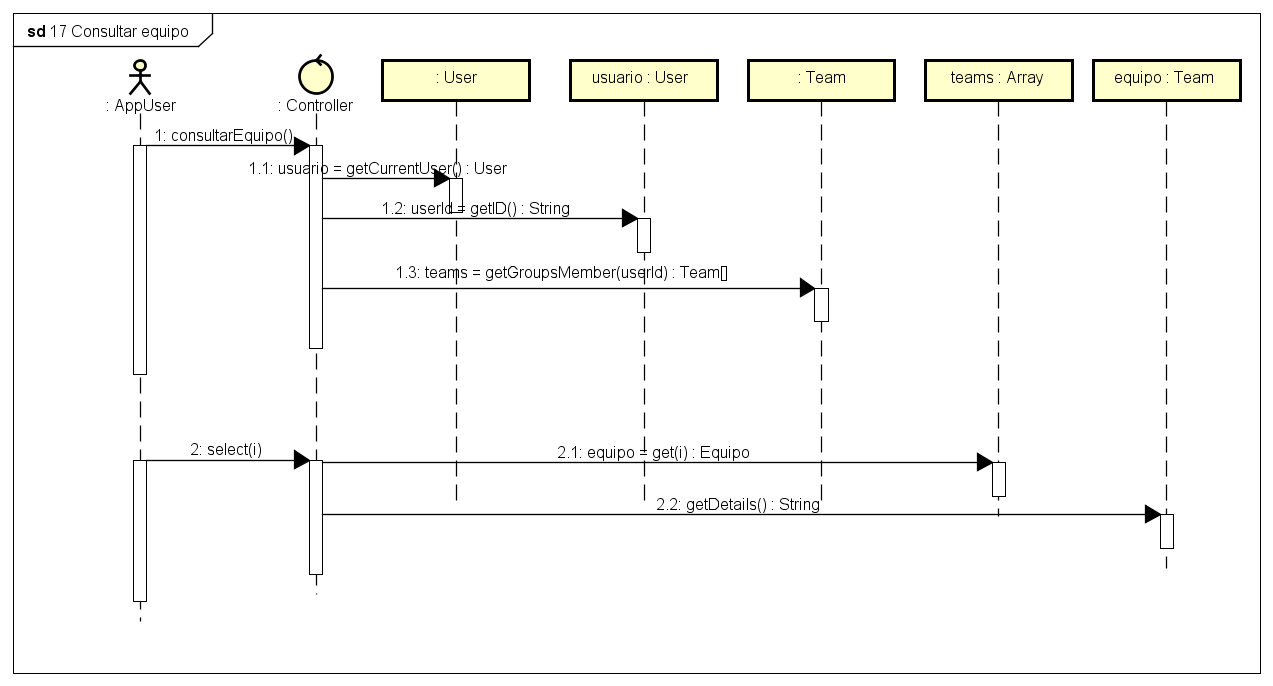
\includegraphics[scale=0.5]{images/sequence/checkTeam}
\caption{Diagrama de secuencia del caso de uso “Consultar equipo“}
\end{figure}

%18
\begin{figure}[H]
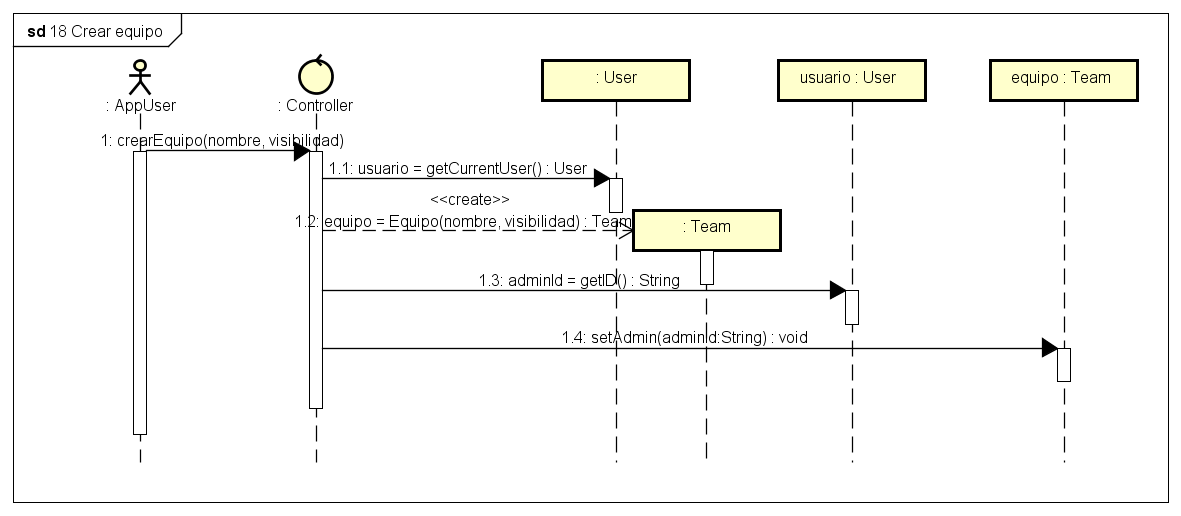
\includegraphics[scale=0.5]{images/sequence/createTeam}
\caption{Diagrama de secuencia del caso de uso “Crear equipo“}
\end{figure}

%19
\begin{figure}[H]
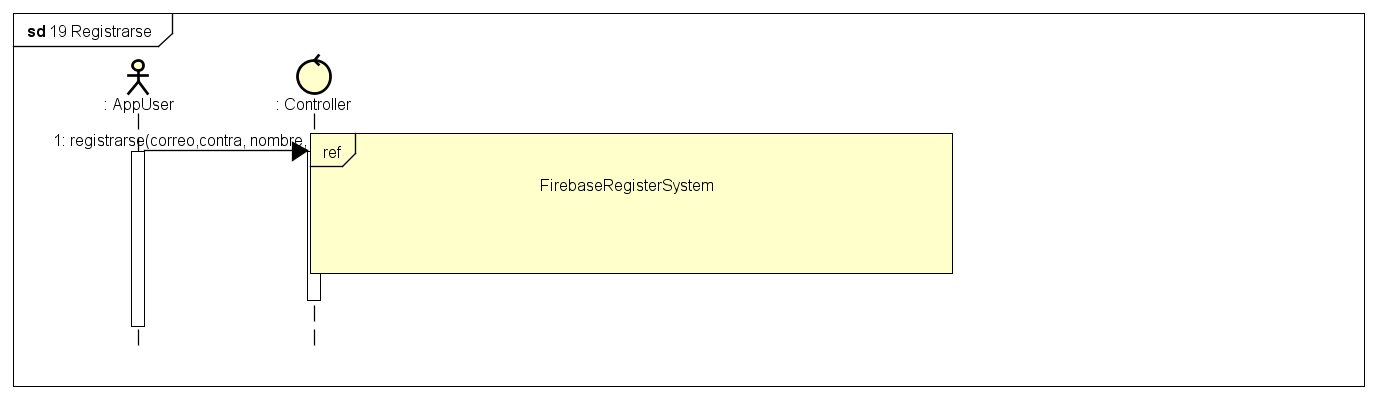
\includegraphics[scale=0.5]{images/sequence/register}
\caption{Diagrama de secuencia del caso de uso “Registrarse“}
\end{figure}


%20
\begin{figure}[H]
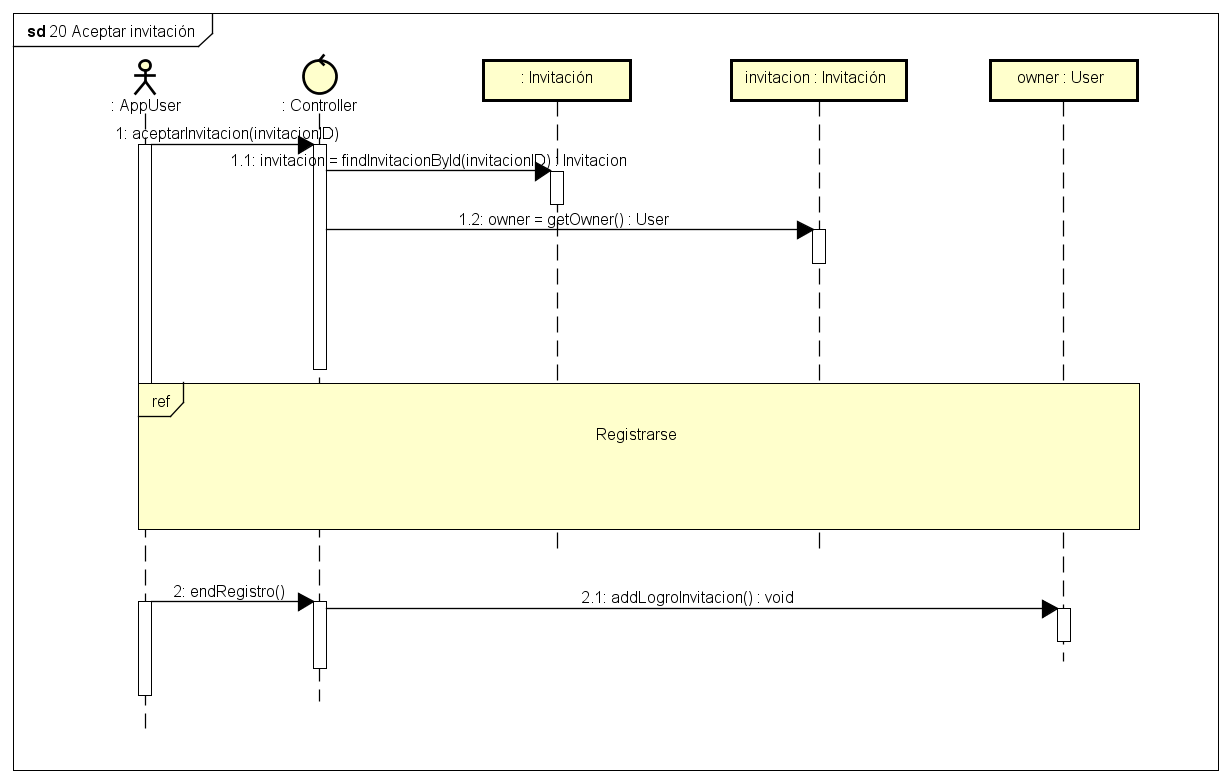
\includegraphics[scale=0.5]{images/sequence/acceptInvitation}
\caption{Diagrama de secuencia del caso de uso “Aceptar invitación“}
\end{figure}

%21
\begin{figure}[H]
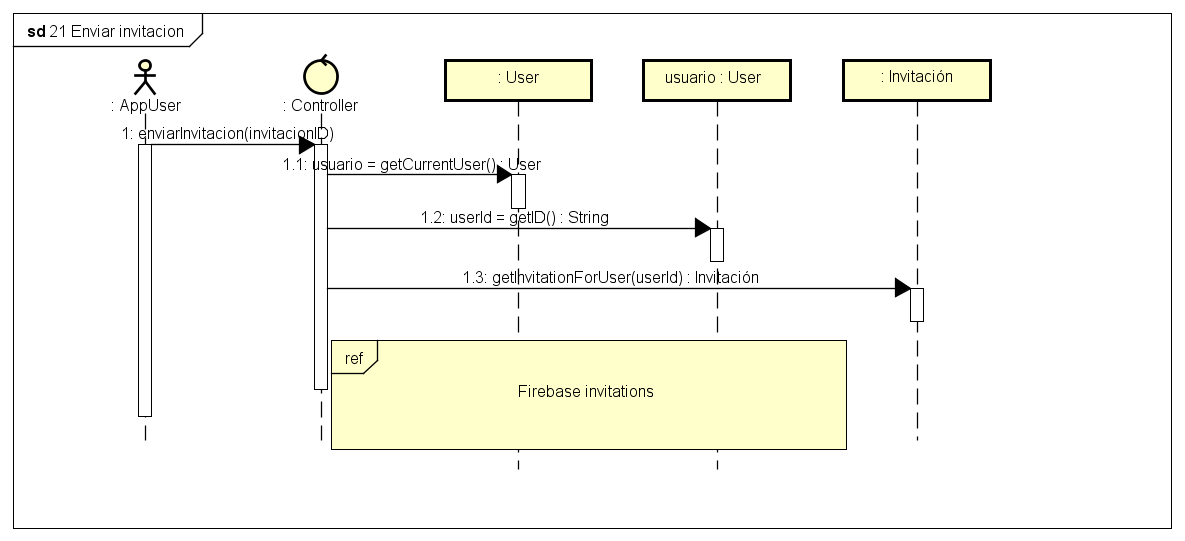
\includegraphics[scale=0.5]{images/sequence/sendInvitation}
\caption{Diagrama de secuencia del caso de uso “Enviar invitación“}
\end{figure}

%22
\begin{figure}[H]
\includegraphics[scale=0.5]{images/sequence/login}
\caption{Diagrama de secuencia del caso de uso “Iniciar sesión“}
\end{figure}

%23
\begin{figure}[H]
\includegraphics[scale=0.5]{images/sequence/showOtherPlayersPositions}
\caption{Diagrama de secuencia del caso de uso “Ver posición de otros jugadores“}
\end{figure}

%23
\begin{figure}[H]
\includegraphics[scale=0.5]{images/sequence/checkPrizes}
\caption{Diagrama de secuencia del caso de uso “Consultar premios“}
\end{figure}


\section{Diseño}
\subsection{Arquitectura}
La aplicación se estructura, a alto nivel en los siguientes paquetes:
\begin{figure}[H]
\centering
\includegraphics[scale=0.5]{images/structureHighLevel}
\caption{Diagrama de paquetes de alto nivel de la aplicación}
\end{figure}

La estructura interna de los paquetes es:

\begin{figure}[H]
\centering
\includegraphics[scale=0.6]{images/structureModel}
\caption{Diagrama de clases \textit{Model}}
\end{figure}

\begin{figure}[H]
\centering
\includegraphics[scale=0.7]{images/structureloginGameModel.PNG}
\caption{Diagrama de clases de los paquetes \textit{LoginActivity} y \textit{GameActivity}}
\end{figure}

\begin{figure}[H]
\centering
\includegraphics[scale=0.6]{images/structureMainActivity}
\caption{Diagrama de clases del paquete \textit{MainActivity}}
\end{figure}

\begin{figure}[H]
\centering
\includegraphics[scale=0.7]{images/structureMissions}
\caption{Diagrama de clases del paquete \textit{MissionsActivity}}
\end{figure}


\begin{figure}[H]
\centering
\includegraphics[scale=0.6]{images/structureTeam}
\caption{Diagrama de clases del paquete \textit{TeamActivity}}
\end{figure}

\subsection{Patrones utilizados}
Se ha decidido emplear los siguientes patrones en el diseño e implementación de la aplicación.

\subsubsection{M.V.C. (Modelo Vista Controlador)}
El M.V.C. es un patrón de arquitectura software utilizado para la implementación de interfaces de usuario (\textit{GUI}). El fundamento de este patrón es el de separar la lógica de la aplicación en tres componentes completamente diferenciados \cite{mvcua}:
\begin{itemize}
\item \textbf{Modelo:} el modelo define la información que contiene la aplicación. Además, deberá tener acceso a un sistema de persistencia que permita acceder a la misma en futuras ocasiones y, en el caso de que el modelo fuera activo, notificará a las vistas de los cambios que ocurrieran sobre el estado, con el fin de que estas refrescaran la información visible al usuario.
\item \textbf{Vista:} define cómo se deberá mostrar la información al usuario.
\item \textbf{Controlador:} controla la lógica de negocio necesaria para leer la información introducida por el usuario en la vista y actualizar el controlador. Similarmente, transformará la información proveniente del modelo para que pueda ser mostrada al usuario por la vista.
\end{itemize}
En el caso de la aplicación Route66App, tanto las vistas como los controladores se encuentran en sus respectivos paquetes, dentro de \textit{Activities}. Sin embargo, parte del modelo es gestionada directamente por Firebase, por lo que en el paquete \textit{model} habrá simplemente clases (\textit{POJO}) que representan a los objetos del modelo.

\subsubsection{DAO (Data Access Object)}

DAO realiza una capa de abstracción entre los servicios y llamadas de bajo nivel para acceder a los datos del resto de código, evitando así mezclar código de diferentes capas.

Este patrón de acceso a datos solo se ha podido emplear en las operaciones CRUD realizadas contra la base de datos que es administrada por \cite{roompersistence} \textit{Room} y no con la que gestiona Firebase Firestore.


\subsection{Esquema de la base de datos}
Como se ha indicado en secciones anteriores, se ha decidido utilizar Firebase como motor de bases de datos. En concreto, de las dos que ofrece la plataforma: Firebase Realtime Database y Firebase Firestore, se ha elegido la segunda ya que es mucho más compleja y permite una mayor personalización. Esta base de datos seleccionada es de tipo no relacional, basada en documentos. \\

Durante el Grado, se ha estudiado la asignatura Diseño de Bases de Datos, impartida por D. Manuel Barrio Solorzano. Sin embargo, esta asignatura se limitaba a enseñar el diseño de bases de datos de tipo relacional y no de tipo no relacional y, al no contar con formación específica en la materia y tras consultar \cite{databasedesign}, se han realizado los siguientes diseños basándose en el libro citado y en diagramas de UML. La \cite{fireference} documentación que Google proporciona en la documentación de Firebase también ha servido de mucha ayuda.

\begin{figure}[H]
\centering
\includegraphics[scale=0.5]{images/databaseNRteams}
\caption{Esquema No Relacional basado en documentos y colecciones para las entidades relacionadas con equipos}
\end{figure}

De la anterior figura se tiene que aclarar la siguiente información:

\begin{enumerate}

\item Entre FirebaseStorageFile y Team no hay una relación directa en la base de datos, si no que se limita a buscar un archivo en el almacenamiento que se llame exactamente igual que la clave del documento que representa al equipo. En caso de existir, diremos que existe esa conexión.

\end{enumerate}

\begin{figure}[H]
\centering
\includegraphics[scale=0.5]{images/databaseNRusers}
\caption{Esquema No Relacional basado en documentos y colecciones para las entidades relacionadas con usuarios}
\end{figure}

Del esquema anterior se deben indicar los siguientes datos:
\begin{enumerate}

\item Al igual que en el caso de los equipos, entre FirebaseStorageFile y User no hay una conexión como tal, sino que esta existe únicamente cuando el fichero se encuentra en este espacio de almacenamiento de archivos.
\item Tampoco existe una conexión en Firestore entre User y FirebaseUser, si no que se va a hacer por medio del identificador único del usuario en Firebase Authentication.

\end{enumerate}


Paralelamente, con el fin de cumplir con los requisitos de persistencia y permitir una actualización de los niveles, también se ha utilizado una base de datos de tipo relacional, gestionada por la biblioteca de persistencia \cite{roompersistence} \textit{Room}. Esta base de datos tendrá como objetivo el de mantener un listado de niveles, misiones así como las sincronizaciones que se hayan hecho para descargarse las nuevas misiones (ver apartado implementación).

\begin{figure}[H]
\centering
\includegraphics[scale=0.5]{images/databaseRoom}
\caption{Esquema de la base de datos relacional gestionada por la biblioteca de persistencia \cite{roompersistence} \textit{Room}}
\end{figure}

\subsection{Diagrama de despliegue}

\begin{figure}[H]
\centering
\includegraphics[scale=0.5]{images/deploymentModel}
\caption{Diagrama de despliegue de la aplicación Android}
\end{figure}

\section{Implementación}

\subsection{Niveles, premios e insignias}
\subsubsection{De usuarios}
Los usuarios de la aplicación contarán con un conjunto de niveles, misiones, premios e insignias que deberán ir obteniendo o completando para avanzar en la aplicación.

Se resume en este apartado aquellos detalles y decisiones que se han tomado al no haberlos encontrados lo suficientemente desarrollados en la memoria del T.F.G. sobre el que está basado este trabajo. 

Los niveles y los detalles concretos de los mismos son los siguientes:

\begin{table}[H]
\resizebox{\textwidth}{!}{%
\begin{tabular}{|l|l|l|l|l|l|l|}
\hline
Nivel & Nombre       & Puntos sociales & Puntos competitivos & Puntos de consumo & Consumo mínimo & Puntuación mínima juego \\ \hline
1     & Chicago      & 500             & 0                   & 0                 & 0 \euro        & 0                       \\ \hline
2     & Springfield  & 300             & 300                 & 300               & 5 \euro        & 300                     \\ \hline
3     & San Louis    & 400             & 400                 & 400               & 10 \euro       & 400                     \\ \hline
4     & Tulsa        & 500             & 500                 & 500               & 15 \euro       & 500                     \\ \hline
5     & Oklahoma     & 600             & 600                 & 600               & 20 \euro       & 600                     \\ \hline
6     & Amarillo     & 700             & 700                 & 700               & 25 \euro       & 700                     \\ \hline
7     & Santa Fe     & 800             & 800                 & 800               & 30 \euro       & 800                     \\ \hline
8     & Alburquerque & 900             & 900                 & 900               & 35 \euro       & 900                     \\ \hline
9     & Flagstaff    & 1000            & 1000                & 1000              & 40 \euro       & 1000                    \\ \hline
10    & Williams     & 1100            & 1100                & 1100              & 45 \euro       & 1100                    \\ \hline
11    & Los Ángeles  & 1200            & 1200                & 1200              & 50 \euro       & 1200                    \\ \hline
\end{tabular}
}
\caption{Misiones del juego junto con sus detalles correspondientes.}
\end{table}

En cada nivel habrá cinco casillas:
\begin{itemize}
    \item Casillas de tipo social: Dependerá del tipo de nivel:
    \begin{itemize}
        \item Nivel 1 (Chicago): Habrá cinco casillas de tipo social, es decir, todas. Cada una vendrá dedicada a un tipo de misión social.
        \item Resto de niveles: Por cada ciudad habrá dos casillas sociales y se considerarán de tipo libre, es decir, el usuario puede elegir qué acción desea realizar para completarla.
    \end{itemize}
    \item Casillas de tipo competitivo: exceptuando el primer nivel habrá dos casillas, cada una será de un juego concreto y su nivel de dificultad irá aumentando gradualmente (la puntuación que se deberá alcanzar será mayor).
    \item Casillas de tipo consumo: habrá una casilla por ciudad (exceptuando en el nivel uno, que no habrá ninguna). El consumo irá aumentando en cada nivel en cinco euros.
\end{itemize}

No se impone que el usuario deba realizar todo el consumo correspondiente a una misión de tipo consumo en una sola ocasión, permitiendo dividirlo en varias ocasiones (siempre y cuando enseñe el código QR correspondiente a la misión concreta). Por otra parte, todo consumo que exceda del indicado (por ejemplo si registra un gasto de 10\euro \vspace{0.1cm} en el nivel Springfield), no será acumulado para la siguiente ciudad.

Igualmente, las insignias y premios que conforman la aplicación son:



\subsection{Explicación de la arquitectura escogida}

Una aplicación Android está basada en cuatro tipos de componentes \cite{androidfund} \cite{androidpacktpub}. Todos deben ser declarados explícitamente en el archivo AndroidManifest.xml:

\begin{enumerate}
\item Actividades: son los elementos más importantes y destacables en una aplicación Android, pues cumplen el papel de interfaz entre la aplicación y la vista.\\
Route66 cuenta con las siguientes actividades:

	\begin{itemize}
	\item \textit{LoginActivity}: sirve para identificar y registrar a los usuarios en de la aplicación (incluyendo aquellos que tienen una invitación). Es la actividad que siempre se lanzará cuando la aplicación sea abierta. Si el usuario ha iniciado sesión, redirigirá  a \textit{MainActivity}.
	
	\item \textit{MainActivity}: es la única actividad que contará con un \textit{DrawerLayout} (el menú principal de la aplicación). De la misma dependen un conjunto de fragmentos (vistas que se acoplan y se desacoplan bajo demanda):
	
		\begin{enumerate}
			\item \textit{Archivements}: es el fragmento encargado de mostrar al usuario el conjunto de logros que haya obtenido.
			
			\item \textit{Insignias}: es el fragmento encargado de mostrar las insignias que haya obtenido el usuario.
			
			\item \textit{Invite}: es el fragmento encargado de servir de interfaz entre la aplicación y el sistema de Firebase Invitations, con el fin de enviar invitaciones.
			
			\item \textit{MainGrid}: es el fragmento encargado de mostrar el conjunto de niveles con los que cuenta la aplicación y servirá como puerta de enlace a realizar misiones y consultar los usuarios que se encuentran en un determinado nivel.
			
			\item \textit{Prizes}: es el fragmento encargado de listar el conjunto de premios que hubiera conseguido el usuario, así como detalles específicos de los mismos.
			
			\item \textit{Profile}: es el fragmento que permite al usuario editar las propiedades de su perfil (avatar, nombre, restaurante favorito, etcétera).
			
			\item \textit{QRCode}: es el fragmento encargado de mostrar el código QR del usuario, con el fin de que posteriormente pueda ser utilizado para añadir un logro de tipo consumo.
			
			\item \textit{SocialRanking}: es el fragmento encargado de mostrar el ranking global de usuarios.
			
			\item \textit{Team}: es el fragmento encargado de listar el conjunto de equipos a los que pertenece el usuario, así como el de permitir crear uno nuevo.
		\end{enumerate}
		
	\item \textit{MissionsActivity}: es la actividad que servirá como interfaz para realizar misiones de tipo consumo, así como de tipo social. 
	
		\begin{enumerate}
		\item \textit{ExpenseMission}: es el fragmento encargado de mostrar al usuario los detalles de una misión de tipo consumo y, si fuera el caso, marcarla como completada.
		
		\item \textit{SocialMission}: es el fragmento encargado de mostrar al usuario los detalles de una misión de tipo social y, si fuera el caso, marcarla como completada.
		\end{enumerate}
		
	\item \textit{GameActivity}: es la actividad que servirá como interfaz para realizar misiones de tipo juego. Por las características de este tipo de misiones (la vista es distinta, así como la posible rotación de la pantalla), se ha decidido separarlas de la actividad \textit{MissionsActivity}.
	\begin{enumerate}
		\item \textit{GameMission}: es el fragmento encargado de mostrar al usuario los detalles de una misión de tipo juego y, si fuera el caso, marcarla como completada.
		\end{enumerate}
		
	\item \textit{NormalActivity}: el objetivo de esta actividad es el de servir como auxiliar a la actividad principal (MainActivity). Es decir, será aquella actividad que será llamada por MainActivity.
	
	\begin{enumerate}
		\item \textit{CreateGroup}: es el fragmento encargado de mostrar el formulario para crear un nuevo grupo.
		\item \textit{HelpFragment}: es el fragmento encargado de mostrar la ayuda en la aplicación.
		\item \textit{LevelDetail}: es el fragmento encargado de mostrar los detalles de un nivel. Su vista está basada en un \textit{TabLayout}, por lo que los fragmentos que se mostrarán en el \textit{ViewPager} son:
		\begin{enumerate}
		\item \textit{MissionsListFragment}: es el fragmento encargado de listar las distintas misiones de un nivel, indicando si han sido previamente completadas o no.
		\item \textit{PeersFragment}: es el fragmento encargado de mostrar el conjunto de usuarios que se encuentran en un determinado nivel. Estos serán miembros de los mismos grupos a los que pertenezca el usuario.
		\end{enumerate}
		\item \textit{SettingsFragment}: es el fragmento encargado de mostrar un panel de configuración básico para ajustar parámetros como el tono de notificación que se deberá utilizar para notificar al usuario.
	\end{enumerate}
	\item \textit{TeamActivity}: es la actividad encargada de mostrar las distintas opciones que cuenta un equipo.
	\end{itemize}

\item Servicios: son componentes que se ejecutan en segundo plano (\textit{background}), tanto de forma automática (por ejemplo, al iniciar el dispositivo) como bajo demanda (mediante una llamada). Se utilizan fundamentalmente para procesar tareas pesadas o que puedan tomar mucho tiempo. A diferencia de las actividades no cuentan con interfaz de usuario, ya que están pensados para ser totalmente transparentes al usuario.\\
Route66App cuenta solo con un servicio:
	\begin{enumerate}
	\item UpdaterService: es utilizado para actualizar la versión en caché de la aplicación de las misiones, niveles, insignias y premios y almacenar estos parámetros en la base de datos SQLite. Por otro lado, los ficheros asociados (en su gran mayoría imágenes), los guarda en una carpeta específica de la aplicación.
	\end{enumerate}

\item Proveedores de contenidos (\textit{“Content providers“}): sirven de interfaz para administrar el acceso a un conjunto compartido de datos de la aplicación, además de proporcionar los mecanismos de seguridad necesarios para ello. Una de sus principales aplicaciones es el de permitir compartir grandes cantidades de información entre procesos, aunque también pueden ser utilizados únicamente por la misma aplicación en la que están contenidos.\\
Route66App no cuenta con ningún proveedor de contenidos.

\item Receptores de mensajes (\textit{“Broadcast receivers“}): este tipo de componente es utilizado para responder ante eventos que ocurran en el sistema (por ejemplo, una falta de disponibilidad de conexión a la red, el arranque del sistema Android, etcétera). El objetivo fundamental de un receptor de mensajes es el de alertar y no el de realizar tareas complejas.
Route66App contará con receptores de mensajes (inicio del sistema).
\end{enumerate}

\subsection{Almacenamiento de datos}

La aplicación utiliza varios tipos de almacenamiento:
\begin{enumerate}
\item En \textit{Firebase Firestore}: es la base de datos principal de la aplicación. Contiene la información necesaria para saber las misiones, los logros o los premios obtenidos, así como para conocer a qué grupos pertenece el usuario y los parámetros de los mismos. Hay una versión almacenada localmente en el dispositivo (\textit{caché)}, que se sincronizará con la parte remota cuando el usuario disponga de una conexión a Internet.

\item En \textit{Firebase Authentication}: gestionará todos los flujos de identificación de usuarios y gestionará el sistema de sesiones.

\item En \textit{Firebase Analytics}: se almacenarán los diferentes datos recogidos por la aplicación, cuyo único interés sea el de realizar estadísticas.

\item En \textit{Google Cloud Messaging}: donde se guardarán y enviarán las diferentes notificaciones que se mostrarán en los dispositivos de los usuarios.

\item En \textit{Firebase Storage}: se utiliza para almacenar los avatares de los usuarios y de los grupos.
\item En una base de datos local SQLite: sirve para almacenar los niveles, insignias, premios y misiones de la aplicación, con sus correspondientes parámetros. De igual forma, también almacenará el historial de sincronizaciones de los mismos. Está gestionada por \cite{roompersistence} la biblioteca de persistencia Room.

\item En ficheros: se utilizan ficheros para mostrar las imágenes de los niveles, los avatares de los usuarios, etcétera (cuando estos se encuentren en la caché). Igualmente, también se requieren ficheros para obtener los niveles y misiones en cuanto el usuario instale la aplicación y no se tenga en ese momento conexión a Internet.

\item En \textit{Shared Preferences}: empleada para el almacenamiento persistente de la configuración de determinados parámetros de la aplicación, como por ejemplo, el tono de notificación.

\item En \textit{Firebase Remote Config}: se almacenará toda la información necesaria para la sincronzación de las misiones, niveles, logros e insignias. 
\end{enumerate}

\subsection{Implementación del modelo}

Tal y como se ha visto en el punto anterior (Almacenamiento de datos) se utilizan varios tipos de almacenamiento dependiendo del tipo de datos que queremos tratar. Se indicarán a continuación los detalles de cada soporte de almacenamiento.

\subsubsection{Firebase Firestore}

Firebase Firestore es la base de datos principal del servicio y en donde se almacena información crucial para el correcto funcionamiento del sistema informático como:
\begin{itemize}
\item Datos sobre las misiones completadas por los usuarios y equipos.
\item Parámetros del perfil del usuario.
\item Premios obtenidos.
\item Insignias recibidas.
\end{itemize} 

Así mismo, el mismo componente ofrece una capa de seguridad por medio de una serie de reglas de seguridad, ya que Firestore internamente realiza cuantas comprobaciones de permisos sean precisas, para asegurar tanto el acceso de lectura, como el de escritura. De esta forma, añadimos al servicio una capa de seguridad muy buena y evitamos tener que recurrir a un backend que no deja de ser otro punto en el que puede haber vulnerabilidades. Estas reglas de permisos aplicadas se adjuntan en el anexo.

\subsubsection{Authentication}

Firebase Authentication es utilizado en el sistema informático para almacenar las sesiones, así como los diferentes métodos de autenticación del usuario en el sistema. Además, es utilizado en primera instancia cuando el usuario se acaba de registrar para recuperar de los proveedores de acceso datos iniciales como su nombre o su correo electrónico.

\subsubsection{Analytics}

Esta parte está enfocada directamente a realizar las estadísticas que pueden ser empleados por la parte de gestión de la aplicación. Para ello se envían datos anonimizados y relacionados con:

\begin{itemize}
\item Intentos de misión.
\item Tiempo de uso de la aplicación.
\item Veces que abre la aplicación.
\item Secciones que más visita.
\end{itemize}

La implementación se hace directamente llamando a los métodos adecuados desde el mismo controlador. El mismo Firebase Analytics por medio de la dirección IP y los datos de sesión (así como la cuenta de Google asociada al terminal Android), es capaz de determinar la ubicación, sexo, versión de la aplicación, versión de Android y franja de edad.

\subsection{Cloud Messaging}

Cloud Messaging es el servicio de notificaciones que Google Cloud ofrece dentro del paquete de Firebase. \\

Las notificaciones pueden ser enviadas, o bien a un dispositivo individual, o bien a un grupo (máximo 20 dispositivos). En el caso de Route66App utilizaremos siempre el envío a un grupo en concreto (todos los grupos de un mismo usuario) por varios motivos:

\begin{enumerate}
\item El usuario puede estar utilizado cualquier dispositivo vinculado a su cuenta. Si la notificación se enviara a uno distinto del que esté usando en ese momento, no la recibirá.

\item Un usuario puede haber cedido su dispositivo a otra persona, o incluso, haber dejado de usarlo. Si no se actualiza en la lista de dispositivos de un usuario, nunca recibirá la notificación.
\end{enumerate}

Un usuario entrará en su grupo de dispositivos en el momento en el que inicie sesión o se registre en Route66App.

\subsubsection{Storage}

Firebase Storage es la parte encargada de almacenar los avatares de usuario y de grupo. Es un almacenamiento de objetos construido sobre Google Cloud Storage. \\

Se ha utilizado la siguiente estructura de archivos:
\begin{itemize}
\item \textit{/avatares}: donde se almacenarán los avatares (imágenes de perfil) de los diferentes usuarios. Para facilitar su identificación cada archivo tendrá como nombre el mismo ID de usuario que asigna Firebase Authentication en el registro (sin extensión). 
\item \textit{/groups}: similar al punto anterior, pero para las imágenes de perfil de los equipos. El identificador de la imagen será la clave del documento del equipo utilizada en la base de datos.
\end{itemize}

Por motivos de escalabilidad y de eficiencia se han establecido los siguientes requisitos:
\begin{itemize}
\item Formatos de imagen: JPG, PNG o GIF.
\item Tamaño máximo: 0.2 MiB.
\end{itemize}

Todas las imágenes subidas al servicio serán previamente redimensionadas para ajustar al tamaño máximo indicado anteriormente. De esta forma se consigue que:

\begin{itemize}
\item Se reduzca la cantidad de datos que se deben transmitir por la red.
\item Se evite tener que tener una función (con el gasto que eso conlleva de tiempo) que realice esta modificación.
\item Se ahorra espacio en Firebase Storage
\end{itemize}

Igualmente, con el fin de reducir el uso de datos y el número de descargas, se realizará una caché de los datos gracias a Glide, un plugin de visualización de imágenes en Android.

\subsubsection{Base de datos local SQLite}

Como se ha indicado anteriormente, se ha decidido utilizar la biblioteca de persistencia Room, ofrecida por Android y muy utilizada en el desarrollo de aplicaciones móviles.

Para su utilización se ha empleado:

\begin{itemize}

\item Un archivo AppDatabase: representa a toda la base de datos SQLite. Es el punto de entrada hacia la misma (sigue el patrón Facade). Con el fin de asegurar que solo haya una única instancia he aplicado el patrón Singleton.
\item DAOs: Un DAO en Room es simplemente una interfaz que incluye la cabecera de cuantos métodos se desee incluir. Tiene una serie de métodos ya implementados y con los que basta añadir una anotación y otros (como consultas SELECT complejas), en los que ya es preciso escribir la consulta completa.
\item Entities: Representan una tabla concreta de la base de datos e incluye como atributos cada uno de los campos que la conforman (incluyendo su tipo, así ciertas propiedades características de una base de datos relacional como el uso de claves primarias o autoincrementos).
\end{itemize}

Esta base de datos es utilizada para mantener una sincronización de las diferentes misiones, niveles, insignias y logros. Se debe recordar que existe un requisito en el que se indicaba que estos debían ser actualizables en cualquier momento por parte del administrador, desde el back-end.

\subsubsection{Ficheros}

Los ficheros resultan de especial importancia para inicializar la base de datos en casos de que la primera vez que el usuario abre la aplicación no tiene conexión o esta es de mala calidad. Se cuentan con los siguientes ficheros:

\begin{itemize}
\item \textit{missions.json}: Incluye el conjunto de niveles y misiones de la aplicación. 

\item \textit{insignias.json}: Incluye las insignias con las que cuenta la aplicación.

\item \textit{prizes.json}: Incluye los diferentes premios existentes en el sistema, junto con la dirección a la imagen que los representa y una breve descripción en castellano.

\end{itemize}

\subsubsection{Shared preferences}

Las preferencias compartidas son un método de persistencia utilizado en Android para el almacenamiento de pequeñas cantidades de datos. Se utilizan en formato clave-valor, por lo que son un mecanismo ideal para el almacenamiento de parámetros de configuración.

En Route66App se han utilizado para guardar únicamente el tono de notificación del usuario, que será el que suene cuando le llegue una notificación entrante proveniente de una confirmación de misión realizada o consumo realizado.

\subsubsection{Firebase Remote Config}

Este producto de Firebase resulta de especial utilidad en aplicaciones en las que se desea que un mismo parámetro de configuración de la aplicación cambie a la vez en todas las instalaciones, o bien, en ciertas específicas que cumplan una determinada condición (por ejemplo, idioma del dispositivo, región o versión de Android instalada). De esta forma, es posible aplicar un determinado ajuste a una franja de usuarios, para comprobar así el efecto que tiene y, en caso de resultar satisfactorio, ir ampliando gradualmente el número de instalaciones con ese parámetro. Cabe destacar que en ningún momento se exige que el usuario se vuelva a instalar o actualizar la aplicación.

En Route66App se ha utilizado este producto para ajustar la URL de los archivos de misiones, premios e insignias, así como la hora y fecha de última actualización de esos archivos.

\subsection{Funciones}

Otro de los aspectos fundamentales de Route66App es el uso de las funciones, muy conocidas en el mundo del \textit{Cloud Computing}. Son pequeños fragmentos de código que son ejecutados en el caso de que ocurra una determinada condición. En Route66App, se ha decidido utilizar Firebase Cloud Functions escuchando a los siguientes eventos:

\begin{enumerate}
\item A las escrituras de \textit{Firebase Firestore}: Es preciso escuchar todos aquellos eventos de escritura y actualización sobre los objetos almacenados en las colecciones de \textit{Achivements} (logros). Esto es necesario para:
	\begin{enumerate}
		\item Poder actualizar la base de datos con la suma de las puntuaciones del usuario.
		\item Poder notificar al usuario en caso de que se le añada un nuevo logro de tipo consumo.
		\item Avisar de que un logro de tipo social ha sido comprobado.
	\end{enumerate}

\item A las llamadas HTTP contra el endpoint (/invitations/{userId}): Este método será ejecutado cuando llegue una llamada GET entrante y anotará en la cuenta del usuario que ha invitado a un usuario.
\end{enumerate}


\begin{figure}[H]
\centering
\includegraphics[width=\textwidth]{images/restAPI}
\caption{Diagrama en el que se muestra la operación \textit{GET}}
\end{figure}

\section{Pruebas}

\newcounter{test}\stepcounter{test}

En el desarrollo de software resultan de especial relevancia las pruebas de código, que pueden ser tanto de caja negra (sin visualizar el código) como de caja blanca. Una de las formas más efectivas de comprobar que aquel código que se modifica no “rompa“ el sistema (es decir, deje de funcionar tal y como está previsto), es mediante el uso de pruebas unitarias que, en Android, se suelen realizar mediante el \textit{framework} \textit{JUnit} \footnote{\url{https://junit.org/junit5/es}}. 

Por otro lado, al hablar de una aplicación con interfaz gráfica también conviene señalar la importancia de las pruebas sobre la interfaz de usuario, que no suelen ser muy conocidas, pues muchos desarrolladores las realizan manualmente, probando la aplicación ellos mismos. En Android contamos con los siguientes frameworks diseñados por Google:

\begin{itemize}
\item \textit{Espresso} \footnote{\url{https://developer.android.com/training/testing/espresso/index.html}} se utilizará cuando tengamos acceso al código fuente de la aplicación (pues se realizan sobre el mismo proyecto de la aplicación). Útil cuando vamos a hacer pruebas sobre nuestra propia aplicación.

\item \textit{UIAutomator} \footnote{\url{https://developer.android.com/training/testing/ui-automator.html}} cuando no tengamos acceso al código fuente (por ejemplo, cuando queremos probar una aplicación de terceros).

\end{itemize}


Sin embargo, en esta aplicación no se realizarán pruebas automatizadas, sino que serán puramente manuales y de caja negra, de acuerdo con los requisitos señalados por la tutora del T.F.G. Estas pruebas son las que describiré con detalle a continuación.

\vspace{1cm}

\begin{test}
  \addheading{\textbf{TEST\arabic{test}}}{El usuario se registra mediante correo electrónico} 
  \addrow{Resultado esperado}{App user.}
  \addrow{Resultado obtenido}{El usuario ha iniciado sesión en el sistema.}
\end{test}\\\stepcounter{test}

\vspace{0.5cm}

\begin{test}
  \addheading{\textbf{TEST\arabic{test}}}{El usuario se registra utilizando Google.} 
  \addrow{Resultado esperado}{}
  \addrow{Resultado obtenido}{}
\end{test}\\\stepcounter{test}

\vspace{0.5cm}

\begin{test}
  \addheading{\textbf{TEST\arabic{test}}}{El usuario inicia sesión mediante correo electrónico.} 
  \addrow{Resultado esperado}{}
  \addrow{Resultado obtenido}{}
\end{test}\\\stepcounter{test}

\vspace{0.5cm}

\begin{test}
  \addheading{\textbf{TEST\arabic{test}}}{El usuario inicia sesión utilizando Google.} 
  \addrow{Resultado esperado}{}
  \addrow{Resultado obtenido}{}
\end{test}\\\stepcounter{test}

\vspace{0.5cm}

\begin{test}
  \addheading{\textbf{TEST\arabic{test}}}{El usuario modifica su configuración de perfil.} 
  \addrow{Resultado esperado}{}
  \addrow{Resultado obtenido}{}
\end{test}\\\stepcounter{test}

\vspace{0.5cm}

\begin{test}
  \addheading{\textbf{TEST\arabic{test}}}{El usuario sube una fotografía de perfil (avatar).} 
  \addrow{Resultado esperado}{}
  \addrow{Resultado obtenido}{}
\end{test}\\\stepcounter{test}

\vspace{0.5cm}

\begin{test}
  \addheading{\textbf{TEST\arabic{test}}}{El usuario completa una misión de tipo social.} 
  \addrow{Resultado esperado}{}
  \addrow{Resultado obtenido}{}
\end{test}\\\stepcounter{test}

\vspace{0.5cm}

\begin{test}
  \addheading{\textbf{TEST\arabic{test}}}{El usuario completa una misión de tipo consumo.} 
  \addrow{Resultado esperado}{}
  \addrow{Resultado obtenido}{}
\end{test}\\\stepcounter{test}

\vspace{0.5cm}

\begin{test}
  \addheading{\textbf{TEST\arabic{test}}}{El usuario completa una misión de tipo competitiva.} 
  \addrow{Resultado esperado}{}
  \addrow{Resultado obtenido}{}
\end{test}\\\stepcounter{test}

\vspace{0.5cm}

\begin{test}
  \addheading{\textbf{TEST\arabic{test}}}{El usuario visualiza los logros recibidos.} 
  \addrow{Resultado esperado}{}
  \addrow{Resultado obtenido}{}
\end{test}\\\stepcounter{test}

\vspace{0.5cm}

\begin{test}
  \addheading{\textbf{TEST\arabic{test}}}{El usuario visualiza las insignias recibidas.} 
  \addrow{Resultado esperado}{}
  \addrow{Resultado obtenido}{}
\end{test}\\\stepcounter{test}

\vspace{0.5cm}

\begin{test}
  \addheading{\textbf{TEST\arabic{test}}}{El usuario visualiza los premios que tiene asignados.} 
  \addrow{Resultado esperado}{}
  \addrow{Resultado obtenido}{}
\end{test}\\\stepcounter{test}

\vspace{0.5cm}

\begin{test}
  \addheading{\textbf{TEST\arabic{test}}}{El usuario visualiza el código QR que tiene asignado.} 
  \addrow{Resultado esperado}{}
  \addrow{Resultado obtenido}{}
\end{test}\\\stepcounter{test}

\vspace{0.5cm}

\begin{test}
  \addheading{\textbf{TEST\arabic{test}}}{El usuario envía una invitación.} 
  \addrow{Resultado esperado}{}
  \addrow{Resultado obtenido}{}
\end{test}\\\stepcounter{test}

\vspace{0.5cm}

\begin{test}
  \addheading{\textbf{TEST\arabic{test}}}{El usuario acepta la invitación y se registra.} 
  \addrow{Resultado esperado}{}
  \addrow{Resultado obtenido}{}
\end{test}\\\stepcounter{test}

\vspace{0.5cm}

\begin{test}
  \addheading{\textbf{TEST\arabic{test}}}{El usuario visualiza su ranking global.} 
  \addrow{Resultado esperado}{}
  \addrow{Resultado obtenido}{}
\end{test}\\\stepcounter{test}

\vspace{0.5cm}

\begin{test}
  \addheading{\textbf{TEST\arabic{test}}}{El usuario visualiza los equipos que tiene asignados.} 
  \addrow{Resultado esperado}{}
  \addrow{Resultado obtenido}{}
\end{test}\\\stepcounter{test}

\vspace{0.5cm}

\begin{test}
  \addheading{\textbf{TEST\arabic{test}}}{El usuario visualiza los logros de un equipo.} 
  \addrow{Resultado esperado}{}
  \addrow{Resultado obtenido}{}
\end{test}\\\stepcounter{test}

\vspace{0.5cm}

\begin{test}
  \addheading{\textbf{TEST\arabic{test}}}{El usuario crea un nuevo equipo.} 
  \addrow{Resultado esperado}{}
  \addrow{Resultado obtenido}{}
\end{test}\\\stepcounter{test}

\vspace{0.5cm}

\begin{test}
  \addheading{\textbf{TEST\arabic{test}}}{El usuario, con rol administrador en un equipo, invita a un usuario.} 
  \addrow{Resultado esperado}{}
  \addrow{Resultado obtenido}{}
\end{test}\\\stepcounter{test}

\section{Manual de instalación}

Manual de instalación

\section{Guía de usuario}
Guía de usuario

\chapter{Conclusiones y trabajo futuro.}
\section{Conclusiones}

Se extraen las siguientes conclusiones a este Trabajo Fin de Grado:
\begin{itemize}

\item Se ha elaborado un sistema informático basado en la ludificación a partir de una idea desarrollada en el T.F.G. de una alumna de nuestra Universidad.

\item Se han aplicado una gran cantidad de conocimientos adquiridos a lo largo del Grado, aunque también me he visto obligado a formarme en otras tecnologías como Kotlin o Firebase.
\end{itemize}

\section{Trabajo futuro}

Se proponen las siguientes ideas para extender las funcionalidades de la aplicación:

\begin{enumerate}
\item Integrar el sistema de ludificación desarrollado en una aplicación que será utilizada en un ambiente real. Un ejemplo podría ser utilizar la cafetería de la Escuela de Ingeniería Informática para ello.

\item Al igual que se ha visto en el estudio de alternativas en el caso de VIPS, permitir pagar la cuenta directamente con saldo recargable. Con cada recarga, el usuario se llevaría una serie de puntos por completar logros de recargas.

\item Poder realizar pedidos directamente desde la aplicación.

\item Realizar la aplicación para la plataforma iOS.

\item Traducir la aplicación a más idiomas, incluyendo el inglés, catalán, euskera, gallego y valenciano.
\end{enumerate}

\chapter{Webgrafía y Bibliografía}

\begin{thebibliography}{a} 
\section{Webgrafía}

\bibitem{iebschoolGami} \textsc{Marc Rodríguez. IEBS Comunidad} \textit{La ludificación como fenómeno social y herramienta global}, Fecha de última visita: 6 de Noviembre de 2017 \url{http://comunidad.iebschool.com/pedrolopezugarte/2015/11/20/la-gamificacion-como-fenomeno-social-y-herramienta-global/}.  

\bibitem{confidencialcorreosgami} \textsc{María Benito} \textit{“Gamificación o cómo lograr que los empleados hagan un trabajo extra gratis“}, Fecha de última visita: 6 de Noviembre de 2017 \url{https://www.elconfidencial.com/empresas/2014-04-27/gamificacion-o-como-lograr-que-los-empleados-hagan-un-trabajo-extra-gratis_121168/}. 

\bibitem{accentureGami} \textsc{Accenture} \textit{Why gamification is serious business}, Fecha de última visita: 6 de Noviembre de 2017 \url{https://www.accenture.com/us-en/insight-outlook-why-gamification-is-serious-business}.  

\bibitem{bbvag} \textsc{Omnium Games.} \textit{BBVA Game: El mayor caso de éxito de la ludificación en España.}, Fecha de última visita: 21 de Noviembre de 2017 \url{http://omniumgames.com/bbva-game-el-mayor-caso-de-exito-de-la-gamificacion-en-espana/}.  

\bibitem{iebsctj} \textsc{Ferran Altarriba Bertran. IEBS School} \textit{Tipos de jugadores en Gamification: teoría Bartle}. Fecha de última visita: 6 de Noviembre de 2017, \url{http://www.iebschool.com/blog/tipos-jugadores-gamification-2-innovacion/}.  

\bibitem{mcdo} \textsc{McDonalds},\textit{Aplicación móvil McDonalds para Android} \url{https://play.google.com/store/apps/details?id=com.mcdonalds.android}

\bibitem{burgerk} \textsc{Burger King},\textit{Aplicación móvil Burger King para Android} \url{https://play.google.com/store/apps/details?id=es.burgerking.android}

\bibitem{kfcapp} \textsc{KFC},\textit{Aplicación móvil KFC para Android} \url{https://play.google.com/store/apps/details?id=es.kfc.spain}

\bibitem{vipsapp} \textsc{VIPS},\textit{Aplicación móvil VIPS para Android} \url{https://play.google.com/store/apps/details?id=com.clubvips.app}

\bibitem{pansapp} \textsc{Pans \& Company},\textit{Aplicación móvil Pans \& Company para Android} \url{https://play.google.com/store/apps/details?id=es.eatout.panscompany}

\bibitem{fostersh} \textsc{Foster's Hollywood},\textit{Aplicación móvil Foster's Hollywood para Android} \url{https://play.google.com/store/apps/details?id=com.zena.Fosters}

\bibitem{androidversiondist} \textsc{Android Developers Official Website},\textit{Dashboards. Platform Versions.} Fecha de última visita: 02 de Diciembre de 2017 \url{https://developer.android.com/about/dashboards/index.html}

\bibitem{infojobs2016} \textsc{Infojobs}. Estado del mercado laboral en España. Año 2016. pág 31. Fecha de última visita: 20/01/2018 \url{http://tueligesinfojobs.net/informe-anual-infojobs-2016.pdf} 

\bibitem{upedu} \textsc{Unified Process for Education. Universidad Politécnica de Montreal}. Fecha de última visita: 25/11/2017 \url{http://www.upedu.org/process/workers/wk_implm.htm}

\bibitem{monopolymcdo} \textsc{McDonalds}. Monopoly Ganador de McDonalds Fecha de última visita: 20/01/2018 \url{https://www.mcdonalds.es/sites/default/files/mcdonalds_lanza_su_nuevo_monopoly_ganador.pdf}

\bibitem{segsocialautonomos} \textsc{Infoautónomos. El Economista}. Tarifa plana de 50 \euro \hspace{0.1cm} para autónomos, jóvenes y mayores de 30. Fecha de última visita: 22/01/2018 \url{https://infoautonomos.eleconomista.es/seguridad-social/tarifa-plana-autonomos-50-euros-mayores-30-jovenes/}

\bibitem{pcuva} \textsc{Universidad de Valladolid. Parque Científico}. Oficinas del Parque Científico de la Universidad de Valladolid. Fecha de última visita: 22/01/2018 \url{http://www.parquecientificouva.es/Upload/ESPACIOS/CTTA/CTTA_FichaOficinas_Jun2013.pdf}

\bibitem{roompersistence} \textsc{Android Developers Official Website}. Room Persistence Library. Fecha de última visita: 23/01/2018 \url{https://developer.android.com/topic/libraries/architecture/room.html}

\bibitem{tapikinull} \textsc{Zhitnitsky, Alex}. The Top 10 Exception Types in Production Java Applications - Based on 1B Events. Fecha de última visita: 08/02/2018 \url{https://blog.takipi.com/the-top-10-exceptions-types-in-production-java-applications-based-on-1b-events}

\bibitem{kotlin} \textsc{Kotlin Programming Language. IntelliJ}. Página Web del lenguaje de programación Kotlin. Fecha de última visita: 08/02/2018 \url{https://kotlinlang.org/}

\bibitem{firebase} \textsc{Firebase}. Página Web de Firebase. Fecha de última visita: 08/02/2018 \url{https://firebase.google.com/}

\bibitem{disadvKotlin} \textsc{Timokhina, Valeria. DZone}. The Pros and Cons of Kotlin for Android Development. Fecha de última visita 08/02/2018. \url{https://dzone.com/articles/the-pros-and-cons-of-kotlin-for-android-developmen}

\bibitem{firebaseadvdis} \textsc{Nathan, Lee. FreeCodeCamp} Firebase Pros and Cons and How to Deal With the Cons. Fecha de última visita 08/02/2018 \url{https://medium.com/@leetheguy/firebase-pros-and-cons-ce37c766190a}

\bibitem{fireference} \textsc{Firebase} Trabajar con arreglos, listas y conjuntos. Fecha de última visita 24/02/2018.  \url{https://firebase.google.com/docs/firestore/solutions/arrays?hl=es-419}

\bibitem{androidfund} \textsc{Android Reference Guide} Aspectos fundamentales de la aplicación. Fecha de última visita 24/02/2018. \url{https://developer.android.com/guide/components/fundamentals.html}



\section{Bibliografía}

\bibitem{cristinatfg} \textsc{Martínez Martínez, Cristina} \textit{T.F.G. “Estudio de ludificación en una empresa para mejorar la fidelización de los clientes”}. Curso 2016-2017. Grado en Ingeniería en Organización Industrial. Universidad de Valladolid. 

\bibitem{anatfg} \textsc{Ruiz Caballero, Ana} \textit{T.F.G. “Estudio de la ludificación de una empresa para incentivar la motivación. “}. Curso 2015-2016. Grado en Ingeniería en Organización Industrial. Universidad de Valladolid. 


\bibitem{pgptema2} \textsc{De la Fuente Redondo, Pablo Lucio}. Departamento de Informática de la UVa. Apuntes de la asignatura Planificación y Gestión de Proyectos. Curso 2017-2018. Tema 2: Planificación de Proyectos.

\bibitem{pgpup} \textsc{De la Fuente Redondo, Pablo Lucio}. Departamento de Informática de la UVa. Apuntes de la asignatura Planificación y Gestión de Proyectos. Curso 2017-2018. Tema 3: Proceso Unificado.


\bibitem{smovkotlin} \textsc{Adiego Rodríguez, Joaquín}. Departamento de Informática de la UVa. Apuntes de la asignatura Sistemas Móviles. Curso 2017-2018. Kotlin.

\bibitem{databasedesign} \textsc{Hills, Ted}. NoSQL and SQL Data Modelling. Bringing together data, semantics and software. Technics Publications.

\bibitem{androidpacktpub} \textsc{Boyer, Rick \& Mew, Kyle}. Android Application Development Cookbook - Second Edition. Over 100 recipes to help you solve the most common problems faced by Android Developers today. PacktPub

\bibitem{mvcua} \textsc{Crespo Carvajal, Yania; Gonzalo Tasis, Margarita; Hernández Díaz, Carmen; Martínez Monés, Alejandra} Modelo vista controlador (MVC). Prácticas. Apuntes de la asignatura Interacción Persona-Computador. Curso 2015-2016. Departamento de Informática de la UVa. Universidad de Valladolid. 

\end{thebibliography}

\chapter{Anexos}

\section{Reglas de seguridad en Firebase}

\section{Prototipos iniciales}

\end{document}